%==========================================================
%-------------------- begin preamble ----------------------
%==========================================================
%\documentclass[12pt]{article}
\documentclass[12pt, a4paper, abstracton]{scrartcl}
\setkomafont{disposition}{\normalfont\bfseries}
\usepackage{Setup/style}
%---------------- custom style -----------------------
%----- equation numbering -------
\numberwithin{equation}{section}     % number within section
%\numberwithin{equation}{subsection} % number within subsection

%----- fig & table numbering -----
\counterwithin{figure}{section}
\counterwithin{table}{section}

%--------- format abstract ---------
\makeatletter
\renewenvironment{abstract}{
    \if@twocolumn
      \section*{\abstractname}
    \else
      \begin{center}
        {\bfseries \large\abstractname\vspace{\z@}}
      \end{center}
      \quotation
    \fi}
    {\if@twocolumn\else\endquotation\fi}
\makeatother

%----------------- tikz ---------------------------
% Define block styles
\tikzstyle{startstop} = [rectangle, rounded corners,
    minimum width=3cm, minimum height=1cm,text centered, draw=black, fill=red!30]
\tikzstyle{io} = [trapezium, trapezium left angle=70, 
    trapezium right angle=110, minimum width=3cm, minimum height=1cm, text centered, text width=3cm, draw=black, fill=blue!30]
\tikzstyle{process} = [rectangle, minimum width=3cm,
    minimum height=1cm, text centered, text width=3cm, 
    draw=black, fill=orange!30] 
\tikzstyle{decision} = [diamond, minimum width=3cm, 
    minimum height=1cm, text centered,text width=2cm, 
    draw=black, fill=green!30]
\tikzstyle{arrow} = [thick,->,>=stealth]
\tikzstyle{block} = [rectangle, draw, fill=blue!20, 
    text width=5em, text centered, rounded corners, minimum height=4em]
\tikzstyle{line} = [draw, -latex']
\tikzstyle{cloud} = [draw, ellipse,fill=red!20, node distance=3cm,
    minimum height=2em]


%---------- insert custom LaTeX commands ----------
\newcommand*{\QED}{\hfill\ensuremath{\square}}
\newcommand{\E}{\mathrm{E}}
\newcommand{\R}{\mathbb{R}}
\newcommand{\X}{\mathbf{X}}
\newcommand{\y}{\mathbf{y}}
\newcommand{\rss}{\mathrm{RSS}}
\newcommand{\MSE}{\mathrm{MSE}}
\newcommand{\Err}{\mathrm{Err}}
\newcommand{\err}{\mathrm{err}}
\newcommand{\bias}{\mathrm{Bias}}
\newcommand{\Var}{\mathrm{Var}}
\DeclareMathOperator*{\argmax}{arg\,max}
\DeclareMathOperator*{\argmin}{arg\,min}
\DeclareMathOperator*{\cv}{CV}
\DeclareMathOperator*{\df}{df}
\newcommand{\T}{\mathcal{T}}

\NewDocumentCommand{\cw}{v}{%
\textbf{\texttt{\textcolor{Blue}{#1}}}%
}


\addbibresource{bibliography.bib}   % Bibliography

% Set graphics path
\graphicspath{{latex/figures/}}

%-------- header & foot -------- 
% FILL IN APPROPRIATE DESCRIPTIONS
% title page
\pagestyle{fancy}
\fancypagestyle{firststyle}
{
   \fancyhf{}
   \fancyfoot[C]{
   % Link to GitHub
   \faGithub \ 
   \href{https://github.com/nicolossus/FYS4411-Project1}{github.com/nicolossus/FYS4411-Project1}}
   \renewcommand{\headrulewidth}{0pt}
   \renewcommand{\footrulewidth}{0.4pt}
}
% rest of document
\fancyhead[L]{\small FYS4411}       % Set <course>
\fancyhead[C]{\small Project 1}             % Set <title>    
\fancyhead[R]{\small May 27, 2022}   % Set <date>
\fancyfoot[C]{-- \thepage\ --}
\renewcommand{\headrulewidth}{0.4pt}
\renewcommand{\footrulewidth}{0.4pt}

% No header:
%\fancyhead{} 
%\renewcommand{\headrulewidth}{0pt}
\usepackage{appendix}
\AtBeginEnvironment{appendices}{\crefalias{section}{appendix}}

%==========================================================
%-------------------- end preamble ----------------------
%==========================================================

%==========================================================
%-------------------- main content ----------------------
%==========================================================
\begin{document}
%------------------ title -------------------------
%================================================================
%------------------------ Title Page ----------------------------
%================================================================
\newcommand{\horrule}[1]{\rule{\linewidth}{#1}} %Horizontal rule
\newcommand{\RNum}[1]{\uppercase\expandafter{\romannumeral #1\relax}}
\titlehead{
\includegraphics[scale=0.35]{latex/latex-report/Images/Logo/FI/MN_FYSISK_Seal_A_ENG.pdf}}
\title{
\large \textsc{FYS4411: Computational Physics II} % Set <COURSE>
\\ [25pt]
\horrule{0.5pt} \\[0.4cm]
\huge Project 1}               % Set <TITLE>
\subtitle{A Variational Monte Carlo Analysis on Bose-Einstein Condensation in a Trapped Bose Gas         % Set <SUBTITLE>
\horrule{2pt} \\[0.5cm]}
\author{Jørn Eirik Betten \and Aleksandar Davidov \and Nicolai Haug}            % Set <AUTHOR>, separate multiple                                 % authors with \and
\date{May 6, 2022}     % Set <DATE>

\maketitle



\pagenumbering{gobble}
\thispagestyle{firststyle}

%---------------- abstract -------------------------
%================================================================
%------------------------- Abstract -----------------------------
%================================================================
\begin{abstract}
In this project, we build a variational Monte Carlo method to estimate the ground state energy of an ultracold, dilute Bose gas in harmonic traps. We use a trial wave function composed of a single particle Gaussian with a single variational parameter and a hard sphere Jastrow factor for pair correlations. We consider two Markov chain Monte Carlo sampling algorithms; a random walk Metropolis with Gaussian proposals and a Langevin Metropolis-Hastings with proposals driven according to the gradient flow of the probability density of the trial wave function. The methods are implemented in a Python framework with automatic differentiation, procedures for tuning scale parameters and gradient descent optimizations of the variational parameter. The blocking method, which accounts for the autocorrelation of a Markov chain, is used to calculate the statistical error of the variational energy. The implementation is verified by comparison with closed-form expressions available when we consider a system of non-interacting bosons only. We find that ... WHICH IS BETTER? RMW OR LMH? AD TIME VS ANALYTICAL? ETC... Our framework provides a solid foundation for building a more general variational Monte Carlo method that can handle more complex systems. 
\end{abstract}   % Abstract on title page
\newpage

%------------ content overview ---------------------
\frontmatter      % Folios in Roman numerals
\tableofcontents    
%\abstractintoc   % Add abstract to table of contents
%\listoffigures      
%\listoftables       
%\listofalgorithms
%\listoftodos       % list TODOs

%----------------- body ----------------------------
\mainmatter         % Folios in Arabic numerals
%================================================================
\section{Introduction}\label{sec:Introduction}
%================================================================

%\newpage 
%================================================================
\section{Theoretical Background}\label{sec:Theory}
%================================================================

%----------------------------------------------------------------
\subsection{Variational Monte Carlo}
%----------------------------------------------------------------

Variational Monte Carlo (VMC) is a method applicable for finding an estimate to the ground state energy of a given quantum mechanical system. It proposes a trial wave function, $\ket{\Psi_T}$, and calculates the expected energy, or any other observable given its operator, by making use of a Monte Carlo evaluation of the integral. The trial wave function is designed with care and hopefully resembles the true wave function in architecture. By adding variational parameters in the trial wave function we may make use of the variational principle such that the energy functional on the trial wave function becomes a convex functional. A convex functional has a single global minimum. Therefore, if our trial wave function architecture resembles the architecture of the ground state wave function, we may simply make a search in the variational parameter space for the minima, and find an upper bound estimate of the exact ground state energy, $E_0$. In the following, we provide the details of the VMC method. 

%---------------------------------------------------------------- 
\subsubsection{Monte Carlo Integration and Expectation Values}\label{sec:mc_integration}
%----------------------------------------------------------------

The general motivation to use Monte Carlo integration in quantum physics is its capability to compute multidimensional definite integrals, that is, integrals on the form 

\begin{equation*}
    I = \int \dd{x_1} \int \dd{x_2} ... \int \dd{x_n} f \qty(x_1, x_2, ..., x_n),
\end{equation*}

where $f \qty(x_1, x_2, ..., x_n)$ is a function in $n$ variables. Fundamental to quantum mechanics is the computation of the expectation value of an observable. In general, for any absolutely continuous stochastic variable $X$ with probability density function (pdf) $p(x)$ over states $x$, the law of the unconscious statistician states that the expectation value of $X$ is given by 

\begin{equation}\label{eq:general_expval}
    \expval{X} = \int_\R x p (x) \dd{x},
\end{equation}

which for quantum systems typically will be a multidimensional integral. The Monte Carlo integration approach to compute the above integral is to sample $M$ possible states $x$ from $p(x)$. The law of large numbers then gives that 

\begin{equation*}
    \expval{X} = \lim_{M \to \infty} \frac{1}{M} \sum_{i=1}^M x_i p \qty(x_i),
\end{equation*}

such that the expectation value can be approximated by

\begin{equation}\label{eq:mc_integration}
    \expval{X} \approx \frac{1}{M} \sum_{i=1}^M x_i p \qty(x_i).
\end{equation}

The number $M$ is usually referred to as the number of Monte Carlo samples or cycles. The estimation error of Monte Carlo integration is independent of the dimensionality of the integral and decreases as $1 / \sqrt{M}$. Monte Carlo integration is therefore more efficient for multidimensional integrals than traditional methods, such as the trapezoidal rule, which typically suffer from the curse of dimensionality. 

When applying Monte Carlo integration, the naive Monte Carlo approach is to sample points uniformly on the phase space and evaluate the pdf at those points. Generally, systems only span a tiny portion of their phase space such that $p(x) \simeq 0$ for most states $x$. The contribution to the expectation value will therefore be negligible for a large portion of the samples, rendering the naive Monte Carlo approach inefficient. There is thus a need for procedures prioritizing sampling toward the values of $x$ that significantly contribute to the expectation value. The family of Markov chain Monte Carlo (MCMC) sampling algorithms have this convergence property and are the predominant choice. The MCMC sampling algorithms used in this project will be discussed in \autoref{sec:sampling_algos}.

For the sake of completeness, we introduce a particularly useful class of expectation values called \textit{moments}. The $n$-th moment of a stochastic variable $X$ with pdf $p(x)$ is defined as 

\begin{equation*}
    \expval{X^n} \equiv \int x^n p(x) \dd{x}.
\end{equation*}

Moments about the mean of the pdf are called \textit{central moments}, and are used in preference to ordinary moments as they describe the spread and shape of the pdf in a  location-invariant manner. The $n$-th central moment is defined as 

\begin{equation*}
    \expval{\qty(X - \expval{X})^n} \equiv \int \qty(x - \expval{x})^n p(x) \dd{x}.
\end{equation*}

The second central moment, known as the variance, is of particular interest. For a stochastic variable $X$, the variance is denoted as $\Var \qty(X)$ and given by 

\begin{equation}
    \Var \qty(X) =  \expval{\qty(X - \expval{X})^2} = \expval{X^2} - \expval{X}^2.
\end{equation}



%---------------------------------------------------------------- 
\subsubsection{Review of the Variational Principle}\label{sec:variational_principle}
%----------------------------------------------------------------

The variational principle (for reference literature see e.g. \cite{VMC}) states that, given a trial wave function $\ket{\Psi_T}$, the energy functional of the wave function has the ground state energy, $E_0$, as a lower bound. Any trial wave function can be expanded in terms of the orthonormal basis set of eigenfunctions of the Hamiltonian operator in Hilbert space, as they form a complete set. Denoting the eigenfunctions as $\ket{\Psi_k}$ and the Hamiltonian as $H$, such that $H\ket{\Psi_k}=E_k\ket{\Psi_k}$, we may expand the trial wave function in this eigenspace

\begin{equation*}
    \ket{\Psi_T} = \sum_{k}c_k\ket{\Psi_k}.
\end{equation*}

Making use of the orthonormality of the basis set, the normalization of the trial wave function is given by

\begin{equation*}
    \braket{\Psi_T} = \sum_k\sum_l c_kc_l\braket{\Psi_k}{\Psi_l} = \sum_k \abs{c_k}^2.
\end{equation*}

The expected value of the Hamiltonian is then given by

\begin{equation*}\label{eq:energy_functional_basis_set}
    \bra{\Psi_T}H\ket{\Psi_T} = \sum_k\abs{c_k}^2E_k
\end{equation*}

and the energy functional can be written as 

\begin{equation}\label{eq:variational_expval}
    \expval{E} = \expval{H} = \frac{\bra{\Psi_T}H\ket{\Psi_T}}{\braket{\Psi_T}} = \frac{\sum_k\abs{c_k}^2E_k}{\sum_k\abs{c_k}^2}, 
\end{equation}

which, since $E_k\geq E_0 \forall k$, shows that the ground state energy is a lower bound of the energy functional. The variance

%The integral which defines the expectation value of the $n$th moment of the Hamiltonian becomes
% Blir ikke denne litt feil? Tror den er riktig. 
%\begin{equation*}
%    \bra{\Psi_T} H \ket{\Psi_T} = \frac{\bra{\Psi_T} H^n \ket{\Psi_T}}{\braket{\Psi_T}} = E_0^n
%\end{equation*} 
%if $\ket{\Psi_T}=\ket{\Psi_0}$ with $\ket{\Psi_0}$ denoting as the ground state. This leads to a variance 

\begin{equation}\label{eq:variational_variance}
    \mathrm{Var}(E) = \frac{\bra{\Psi_T}H^2\ket{\Psi_T}}{\braket{\Psi_T}} -\qty(\frac{\bra{\Psi_T}H\ket{\Psi_T}}{\braket{\Psi_T}})^2,
\end{equation}

becomes zero when $\ket{\Psi_T}$ is equal to the (generally not normalized) ground state. Thus, we know we have the exact ground state energy if the variance of the expectation value of the energy is zero. 


%---------------------------------------------------------------- 
\subsubsection{The Variational Monte Carlo Method}
%---------------------------------------------------------------- 

The first step of the VMC method is to formulate a trial wave function, $\Psi_T \qty(\bm{r}; \bm{\alpha})$, where $\bm{r} = \qty(\bm{r}_1, \bm{r}_2, ..., \bm{r}_N)$ denotes the spatial coordinates, in total $d\times N$ if we have $N$ particles in $d$ dimensions present, and $\bm{\alpha} = \qty(\alpha_1, \alpha_2, ..., \alpha_m)$ the variational parameters. The next step is to evaluate the expectation value of the energy given by \autoref{eq:variational_expval}. In order to bring Monte Carlo integration (\autoref{eq:mc_integration}) to the quantum realm, we need to bring \autoref{eq:variational_expval} to an expression on the form of \autoref{eq:general_expval}. By noting that the trial wave function defines the quantum pdf as 

\begin{equation}\label{eq:wf_pdf}
    p \qty(\bm{r}; \bm{\alpha}) = \frac{\abs{\Psi_T \qty(\bm{r}; \bm{\alpha})}^2}{\int \dd{\bm{r}} \abs{\Psi_T \qty(\bm{r}; \bm{\alpha})}^2}
\end{equation}

and introducing the local quantum operator known as the \textit{local energy}

\begin{equation}\label{eq:variational_local_energy}
    E_L \qty(\bm{r}; \bm{\alpha}) \equiv \frac{1}{\Psi_T \qty(\bm{r}; \bm{\alpha})} H \Psi_T \qty(\bm{r}; \bm{\alpha}),
\end{equation}

we can write the expectation value of the energy as 

\begin{equation}
    \expval{E} = \int \dd{\bm{r}} E_L \qty(\bm{r}; \bm{\alpha}) p \qty(\bm{r}; \bm{\alpha}).
\end{equation}

Monte Carlo integration can then be applied, and the approximation takes the form

\begin{equation}
    \expval{E} \approx \frac{1}{M} \sum_{i=1}^M E_L \qty(\bm{r}_i; \bm{\alpha}) p \qty(\bm{r}_i; \bm{\alpha}).
\end{equation}


The final step of the VMC method is to vary $\bm{\alpha}$ while re-evaluating the expectation value of the energy until it yields the minimum possible energy. For a convex functional, gradient descent optimization may be used to find the direction in the variational parameter space which lowers the expected value of the energy and update the variational parameters in that direction. We discuss gradient descent optimization in \autoref{sec:gradient_descent}.

% Removing this for now
%\autoref{alg:vmc} summarizes the VMC method.

%\begin{algorithm}
%\caption{Variational Monte Carlo}
%\begin{algorithmic}[1]
%\State $\Psi_T(\alpha)$\Comment{Stating a trial wave function.}
%\State $\mathbb{E}[E_L], \nabla_{\alpha}\mathbb{E}[E_L]\gets$ MCSampling($\Psi_T(\alpha)$)\Comment{Finding expected values of the energy and gradient w.r.t. variational parameters, $\alpha$.}
%\State Update $\alpha$. 
%\end{algorithmic}
%\label{alg:vmc}
%\end{algorithm}

% OLD

%To summarize what the Variational Monte Carlo method is; first, we state a trial wave function, $\Psi_T(\vb{R}; \alpha)$. The next step is evaluate the expectation value of the energy functional. We will evaluate the \textit{local energy},

%\begin{equation}\label{eq:local_energy}
%    \mathrm{E}_{\mathrm{L}} = \frac{H\Psi_T(\vb{R};\alpha)}{\Psi_T(\vb{R};\alpha)},
%\end{equation}

%for each step in the sampling process, and averaging over all samples. The third step depends on the optimization method, but a gradient descent method is often used by finding the direction in variational parameter space which lowers the expected value of the local energy, and updating the variational parameters in that direction. The direction is found by finding the gradient with respect to the variational parameters of the expectation value of the local energy. We stop the parameter search by some stopping criterion, e.g. a minimum difference in the variational parameters after an update. 

%Another quantity, the \textit{drift force},  
%\begin{equation}\label{eq:drift_force}
%    \vb{F(\vb{R};\alpha)} = \frac{\nabla_{\vb{R}}\Psi_T(\vb{R};\alpha)}{\Psi_T(\vb{R};\alpha)},
%\end{equation}
%is useful if we use the Metropolis-Hastings sampling algorithm. 


%----------------------------------------------------------------
\subsection{The System}
%---------------------------------------------------------------- 

The system under investigation is a trapped Bose gas of alkali atoms, specifically $^{87}$Rb. A key feature of alkali systems is that they are dilute, i.e., the volume per atom is much larger than the volume of the atom. The average distance between the atoms is thus much larger than the range of the inter-atomic interaction and the physics is dominated by two-body collisions. 

%---------------------------------------------------------------- 
\subsubsection{Bosons in a Harmonic Trap}
%---------------------------------------------------------------- 

In order to model the Bose gas, we consider atoms trapped in either a spherical (S) or elliptical (E) harmonic oscillator trap: 

\begin{equation}\label{eq:Vtrap}
    V_\mathrm{trap} \qty(\bm{r}) = 
    \begin{cases}
        \frac{1}{2} m \omega_\mathrm{ho}^2 r^2 \quad &\text{(S)}
        \\
        \frac{1}{2} m \qty[\omega_\mathrm{ho}^2 \qty(x^2 + y^2) + \omega_z^2 z^2] \quad &\text{(E)}
    \end{cases}.
\end{equation}

Here, $\omega_\mathrm{ho}^2$ defines the trap potential strength. In the case of an elliptical trap, $\omega_\mathrm{ho}=\omega_\perp$ is the trap frequency in the $xy$ plane and $\omega_z$ the frequency in the $z$ direction. The atoms are modeled as hard spheres with a diameter proportional to the scattering length, $a$, that cannot overlap in space, mimicking the strong repulsion that atoms experience at close distances. The two-body interaction between atoms is thus described by the following pairwise, repulsive potential:

\begin{equation}\label{eq:Vint}
    V_\mathrm{int} \qty(\norm{\bm{r}_i - \bm{r}_j}) = 
    \begin{cases}
        \infty, \quad &\norm{\bm{r}_i - \bm{r}_j} \leq a
        \\
        0, \quad &\norm{\bm{r}_i - \bm{r}_j} > a
    \end{cases},
\end{equation}

where $\norm{\cdot}$ denotes the Euclidean distance. The Hamiltonian for a system of $N$ trapped atoms is then given by

\begin{equation}\label{eq:full_hamiltonian}
    H = - \frac{\hbar}{2m} \sum_{i=1}^{N} \grad^2_i + \sum_{i=1}^{N} V_\mathrm{trap}\qty(\bm{r}_i) + \sum_{i < j}^{N} V_\mathrm{int} \qty(\norm{\bm{r}_i - \bm{r}_j}),
\end{equation}

where the notation $i<j$ under the last summation sign signifies a double sum running over all pairwise interactions once. 

%---------------------------------------------------------------- 
\subsubsection{Constructing the Trial Wave Function}
%---------------------------------------------------------------- 

The trial wave function is chosen to take the form of a Slater-Jastrow wave function: 

\begin{equation}\label{eq:twf}
    \Psi_T \qty(\bm{r}; \alpha) = \Phi \qty(\bm{r}; \alpha) J \qty(\bm{r}),
\end{equation}

where $\alpha$ is a variational parameter. The Slater permanent, $\Phi \qty(\bm{r}; \alpha)$, is given by the first $N$ single-particle wave functions chosen to be proportional to the harmonic oscillator function for the ground state: 

\begin{equation}\label{eq:slater}
    \Phi \qty(\bm{r}; \alpha) = \prod_{i=1}^N \phi \qty(\bm{r}_i; \alpha) = \prod_{i=1}^N \exp{-\alpha \qty(x_i^2 + y_i^2 + \beta z_i^2)}.
\end{equation}

Here, $\beta$ could also be a variational parameter. However, in this project we will not treat $\beta$ as a variational parameter, i.e., we limit ourselves to a single variational parameter, $\alpha$. For elliptical traps we set $\beta=2.82843$. For spherical traps we have $\beta = 1$ such that

\begin{equation}\label{eq:slater_spherical}
    \Phi \qty(\bm{r}; \alpha) =  \prod_{i=1}^N \exp{-\alpha \abs{\bm{r}_i}^2} \quad \text{(S)}.
\end{equation} 

The Jastrow correlation factor, $J(\bm{r})$, is chosen to be the exact solution of the Schrödinger equation for interacting pairs of hard spheres atoms:

\begin{equation}\label{eq:jastrow_factor}
    J \qty(\bm{r}) = \prod_{i<j}^N f \qty(a, \norm{\bm{r}_i - \bm{r}_j}),
\end{equation}

where the correlation wave functions are given by

\begin{equation}\label{eq:corr_wf}
    f \qty(a, \norm{\bm{r}_i - \bm{r}_j}) = 
    \begin{cases}
        0 \quad &\norm{\bm{r}_i - \bm{r}_j} \leq a
        \\
        1 - \frac{a}{\norm{\bm{r}_i - \bm{r}_j}} \quad &\norm{\bm{r}_i - \bm{r}_j} > a
    \end{cases}.
\end{equation}

In practice, with this formulation of the correlation wave functions, the inclusion of the repulsive potential (\autoref{eq:Vint}) in the Hamiltonian (\autoref{eq:full_hamiltonian}) becomes redundant as the correlation wave functions yield a probability density of zero whenever $\norm{\bm{r}_i - \bm{r}_j} \leq a$. For non-interacting bosons, $a=0$. 


%---------------------------------------------------------------- 
\subsubsection{Drift Force and One-Body Densities}
%---------------------------------------------------------------- 

Here, we introduce quantities that will be important moving forward. First is the \textit{drift force} of the system given by

\begin{equation}\label{eq:drift_force}
    \bm{F} \qty(\bm{r}; \alpha) = \frac{2 \grad \Psi_T \qty(\bm{r}; \alpha)}{\Psi_T \qty(\bm{r}; \alpha)}.
\end{equation}

The drift force comes into play in the Langevin Metropolis-Hastings sampling algorithm (\autoref{sec:lmh}) as a part that allows the algorithm to traverse the configuration space efficiently by moving towards regions of high probability density.


%One-body density - Tar du denne Jørn?
The \textit{one-body density}, $\rho(\bm{r})$, displays the density of particles in configuration space. Its true form is given by the true ground state wave function $\Psi_0$, where we integrate out all the other particles in the following way

\begin{equation}\label{eq:one_body_density}
    \rho(\bm{r}) =\int_{\bm{r}_2}\int_{\bm{r}_3}\dots\int_{\bm{r}_{N}}\abs{\Psi_0}^2\mathrm{d}\bm{r}_2\mathrm{d}\bm{r}_3 \dots \mathrm{d}\bm{r}_N. 
\end{equation}

This is a simplification which we have done because the system of Bose gas contains identical particles. We recognize the spherical symmetry of our system and instead calculate the \textit{radial one-body density}, $\rho(r)$, where $r=\norm{r}$. This multidimensional integral is evaluated using Monte Carlo integration (see \autoref{sec:mc_integration}), and the radial one-body density is in practice calculated by making a grid of position values and bins of radial distances. We then count the number of samples from the Monte Carlo simulation that matches each bin, and we obtain the approximated one-body density. 


%---------------------------------------------------------------- 
\subsubsection{Scaling and Optimization}\label{sec:Theory_scaling_and_opt}
%---------------------------------------------------------------- 

In our computations, we use natural $\hbar = c =  m = 1$ in order to avoid computing with small numbers as they quickly can lead to large numerical errors. Furthermore, inspired by \cite{FermiNet}, we perform computations with the trial wave function in the log domain. The reason for this is two-fold. Firstly, the form of expressions that need to be evaluated becomes easier. Secondly, the use of logarithmic densities in the MCMC algorithms (see \autoref{sec:sampling_algos}) avoid computational over- and underflows as the evaluation of the ratio between the densities in the common formulation of the algorithms is then computed as the difference of the log densities. In the log domain, the trial wave function of \autoref{eq:twf} assumes the form

\begin{equation}\label{eq:logwf}
\begin{aligned}
  \ln \Psi_T \qty(\bm{r}; \alpha) &= \prod_{i=1}^N \ln \phi \qty(\bm{r}_i; \alpha)  \prod_{i<j}^N \ln f \qty(a, \norm{\bm{r}_i - \bm{r}_j}) \\ 
  &= \sum_{i=1}^N \ln \phi \qty(\bm{r}_i; \alpha)  + \sum_{i<j}^N \ln f \qty(a, \norm{\bm{r}_i - \bm{r}_j}),
\end{aligned}
\end{equation} 

where 

\begin{equation*}
    \ln \phi \qty(\bm{r}_i; \alpha) = -\alpha \qty(x_i^2 + y_i^2 + \beta z_i^2).
\end{equation*}

By using the relation $\Psi_T^{-1} \grad \Psi_T = \grad \ln \Psi_T$, the drift force of \autoref{eq:drift_force} can be written as 

\begin{equation}\label{eq:log_drift_force}
    \bm{F} \qty(\bm{r}; \alpha) = 2 \grad \ln \Psi_T \qty(\bm{r}; \alpha).
\end{equation}

With natural units and in the log domain, the local energy defined by \autoref{eq:variational_local_energy} is given by

\begin{equation}\label{eq:local_energy}
\begin{aligned}
    E_L \qty(\bm{r}; \alpha) &= \Psi_T \qty(\bm{r}; \alpha)^{-1} H \Psi_T \qty(\bm{r}; \alpha) \\
    &= - \frac{1}{2} \sum_{i=1}^N \qty[\grad_i^2 \ln \Psi_T \qty(\bm{r}; \alpha) + \qty(\grad_i \ln \Psi_T \qty(\bm{r}; \alpha))^2] + \sum_{i=1}^{N} V_\mathrm{trap}\qty(\bm{r}_i), 
\end{aligned}
\end{equation}

where we have used that $\Psi_T^{-1} \grad^2 \Psi_T = \grad^2 \ln \Psi_T + \qty(\grad \ln \Psi_T)^2$. The easiest approach to show that the latter relation holds is with the right-hand side as the point of departure;

\begin{align*}
    \grad^2 \ln{\Psi_T} + \qty(\grad\ln{\Psi_T})^2 &= \grad\cdot\grad\ln{\Psi_T} + \grad\ln{\Psi_T}\cdot\grad\ln{\Psi_T}
    \\
    &= \grad\cdot\qty(\frac{1}{\Psi_T}\grad\Psi_T) + \qty(\frac{1}{\Psi_T}\grad\Psi_T)\cdot\qty(\frac{1}{\Psi_T}\grad\Psi_T)
    \\
    &= -\qty(\frac{1}{\Psi_T^2}\grad\Psi_T\cdot\grad\Psi_T) + \qty(\frac{1}{\Psi_T}\grad^2\Psi_T) + \qty(\frac{1}{\Psi_T^2}\grad\Psi_T\cdot\grad\Psi_T)
    \\
    &= \frac{1}{\Psi_T}\grad^2\Psi_T,
\end{align*}

where we again have used the relation $\Psi_T^{-1} \grad \Psi_T = \grad \ln \Psi_T$ and the product rule. 

As mentioned in the introduction, the harmonic oscillator length $a_\mathrm{ho} \equiv \qty[\hbar / \qty(m \omega_\mathrm{ho})]^{1/2}$ provides a characteristic length of the system. Without applying natural units, we introduce the scaling $\bm{r}^* = \bm{r}/a_\mathrm{ho} \Rightarrow \bm{r} = \bm{r}^* a_\mathrm{ho}$. For brevity, we let $\bm{r}^* \to \bm{r}$ so that the preceding notation remains the same. With this scaling, the harmonic oscillator potentials (\autoref{eq:Vtrap}) become 

\begin{equation*}
    V_\mathrm{trap} \qty(\bm{r}) = 
    \begin{cases}
        \frac{1}{2} \hbar \omega_\mathrm{ho} r^2 \quad &\text{(S)}
        \\
        \frac{1}{2} \qty[\hbar \omega_\mathrm{ho} \qty(x^2 + y^2) + \hbar \omega_\mathrm{ho} \frac{\omega_z^2}{\omega_\mathrm{ho}^2} z^2] \quad &\text{(E)}
    \end{cases}.
\end{equation*}

With the energy measured in units $\hbar \omega_\mathrm{ho}$, the harmonic oscillator potentials further simplify to 

\begin{equation}
    V_\mathrm{trap} \qty(\bm{r}) = 
    \begin{cases}
        \frac{1}{2} r^2 \quad &\text{(S)}
        \\
        \frac{1}{2} \qty[x^2 + y^2 + \gamma^2 z^2] \quad &\text{(E)}
    \end{cases},
\end{equation}

where $\gamma = \omega_z / \omega_\mathrm{ho}$. As in \cite{DuBois2001} and \cite{Nilsen2005}, we will use $\gamma = \beta=2.82843$ and $a = a_\mathrm{Rb} / a_\mathrm{ho} = 4.33 \cdot 10^{-3}$.  


%Scaling

%We scale by aho. However, for brevity, we will denote xstar as x, i.e., $r \to r / a_\mathrm{ho}$.

%Then we only need to state the Hamiltonian in exercise g), which only applies to elliptical HO, and (a =) arb/aho = 4.33e-3


%In our code implementation we use the natural units $\hbar = c =  m = 1$. This is done to avoid working with very small numbers, which could lead to large numerical errors. The spherical harmonic oscillator potential has the characteristic length of $a_{\mathrm{ho}}=\sqrt{\frac{\hbar}{m\omega}}$, where $\omega$ is the angular frequency of the oscillator potential (see e.g. \cite{Dalfovo1999}). This is a characteristic length unit for this system. We scale the positions in all arrays to be in units of $a_{\mathrm{ho}}$. That is, 

%\begin{equation*}
%    x_* = \frac{x}{a_{\mathrm{ho}}}, 
%\end{equation*}

%where $x$ is one dimension, and $\hat{x}$ is our scaled dimension length. The single particle part of the Hamiltonian in one dimension then becomes

% Gir feilmelding
%\begin{equation}
%    H = -\frac{\hbar^2}{2ma^2_{\mathrm{ho}}}\dv[2]{x_*} + \frac{m\omega a^2_{\mathrm{ho}}}{2}x_*^{2}.
%\end{equation}

%When natural units are applied, the characteristic length is simplified to $a_{\mathrm{ho}}=\omega^{-\frac{1}{2}}$, and we set the angular frequency of the system to $\omega=1$. The Hamiltonian for a single particle in one-dimensional space is then significantly simplified to 

% Gir feilmelding
%\begin{equation}
%    H = -\frac{1}{2}\dv[2]{x_*} + \frac{1}{2}x_*^{2}, 
%\end{equation}

%which generalizes to $N$ particles in $D$-dimensional space as 

% Gir feilmelding
%\begin{equation}
%    H = -\frac{D}{2}\sum_{i=1}^{N}\qty(\laplacian_{*,i}-\bm{r_{*,j}}\vdot\bm{r_{*,n}}) + \sum_{i<j}^{N}V_{\mathrm{int}}\qty(\norm{\bm{r_{*,i}}-\bm{r_{*,j}}}).
%\end{equation}

%The two-body potential $V_{\mathrm{int}}$ remains the same when the hard sphere diameter $a$ is expressed in terms of $a_{\mathrm{ho}}$ aswell. 



%----------------------------------------------------------------
\subsubsection{Closed-Form Expressions for Non-Interacting Bosons}
%---------------------------------------------------------------- 

In the following, we derive closed-form expressions for a non-interacting system of $N$ bosons trapped in a $d$ dimensional spherical harmonic oscillator. In this case, the trial wave function is given by 

\begin{equation*}
    \ln \Psi_T \qty(\bm{r}; \alpha) =  -\alpha \sum_{i=1}^N \abs{\bm{r}_i}^2, 
\end{equation*}

where $\bm{r} \in \R^{N\times d}$. In spherical coordinates, the gradient of the trial wave function for particle $i$ is given by the radial derivative

% J: Vet ikke helt om dette stemmer. Mangler vi ikke to dimensjoner, eller må spesifisere symmetri? 
% N: Skal være fikset nå

\begin{equation*}
    \grad_i = \pdv{\bm{r}_i}
\end{equation*}

and the Laplacian by its two radial derivative terms in $d$ dimensions; 

\begin{equation*}
    \grad_i^2 = \frac{1}{\bm{r}_i^{d-1}} \pdv{\bm{r}_i} \qty(\bm{r}_i^{d-1} \pdv{\bm{r}_i}). 
\end{equation*} 

Thus, we have that 

\begin{equation*}
    \grad_i \ln \Psi_T \qty(\bm{r}_i; \alpha) = -2 \alpha \bm{r}_i 
\end{equation*} 

and 

\begin{equation*}
    \grad_i^2 \ln \Psi_T \qty(\bm{r}_i; \alpha) = \frac{1}{\bm{r}_i^{d-1}} \pdv{\bm{r}_i} \qty(-2 \alpha \bm{r}_i^d) = \frac{1}{\bm{r}_i^{d-1}}  \qty(-2 d \alpha \bm{r}_i^{d-1}) = -2 d \alpha .
\end{equation*}

The local energy (\autoref{eq:local_energy}) is then given by 

\begin{equation}
    E_L  \qty(\bm{r}; \alpha) = -\frac{1}{2} \sum_{i=1}^N \qty[- 2d \alpha + \qty(-2\alpha \bm{r}_i)^2] + \sum_{i=1}^N \frac{1}{2} \bm{r}_i^2 = Nd \alpha + \sum_{i=1}^N \bm{r}_i^2 \qty(\frac{1}{2} - 2 \alpha^2).
\end{equation}

As $\sum_i \bm{r}_i^2$ is always positive, setting $\alpha = 1 /2$ gives the minimal local energy;

\begin{equation}
    E_L^\mathrm{min} = \frac{d N}{2}.
\end{equation}

The the drift force vector (\autoref{eq:drift_force}) is given by 

\begin{equation}
    \bm{F}\qty(\bm{r}; \alpha) = - 4 \alpha \bm{r}.
\end{equation}



%----------------------------------------------------------------
\subsubsection{Closed-Form Expressions for Interacting Bosons}\label{sec:analytical_interact}
%---------------------------------------------------------------- 

In the case of interacting bosons, we use the following formulation of the trial wave function;

\begin{equation*}
    \ln \Psi_T \qty(\bm{r}; \alpha) = \sum_{i=1}^N \ln \phi \qty(\bm{r}_i ; \alpha) + \sum_{i<j}^N u \qty(r_{ij}),
\end{equation*}

where $u \qty(r_{ij}) \equiv \ln f \qty(a, r_{ij})$ and $r_{ij} \equiv \norm{\bm{r}_i - \bm{r}_j}$. In the ensuing derivations, the aim is to find analytical expressions for the gradient and Laplacian of the trial wave function for a particle $k$. In order to compute $\grad_k u \qty(r_{kj})$, we can rewrite the gradient operator as 

\begin{equation*}
    \grad_k = \grad_k \pdv{r_{kj}}{r_{kj}} = \grad_k r_{kj} \pdv{r_{kj}} = \frac{\bm{r}_k - \bm{r}_j}{r_{kj}} \pdv{r_{kj}} .
\end{equation*}

The gradient of the Slater permanent for particle $k$ is simply the gradient of the single-particle element in question. As the gradient of the pairwise correlations only acts on particle $k$, the only non-zero interactions will involve particle $k$. Thus, the gradient of the trial wave function for particle $k$ is 

\begin{equation}
\begin{aligned}
    \grad_k \ln \Psi_T \qty(\bm{r}; \alpha) &= \grad_k \ln \phi \qty(\bm{r}_k; \alpha) + \sum_{j \neq k}^N \grad_k u \qty(r_{kj}) 
    \\
    &= \grad_k \ln \phi \qty(\bm{r}_k; \alpha) + \sum_{j \neq k}^N \frac{\bm{r}_k - \bm{r}_j}{r_{kj}} u' \qty(r_{kj}),
\end{aligned}
\end{equation} 

where $u' \qty(r_{kj}) \equiv \pdv{r_{kj}} u \qty(r_{kj})$ and the summation $\sum_{j\neq k}$ signifies that each interaction with particle $k$ is enumerated only once, and self-interaction is excluded from the summation. 

As with the gradient, the Laplacian of the Slater permanent is simply $\grad_k^2 \ln \phi \qty(\bm{r}_k; \alpha)$. The Laplacian of the pairwise correlations, on the other hand, is more involved to derive. Our point of departure is 

\begin{equation}\label{eq:int_lap_wip}
\begin{aligned}
    \grad_k \sum_{j\neq k}^N \grad_k u \qty(r_{kj}) &= \sum_{j \neq k}^N \grad_k  \qty( \frac{\bm{r}_k - \bm{r}_j }{r_{kj}} u' \qty(r_{kj}))
    \\
    &= \sum_{j \neq k} \qty(u' \qty(r_{kj})\grad_k  \qty( \frac{\bm{r}_k - \bm{r}_j }{r_{kj}}) + \frac{\bm{r}_k - \bm{r}_j }{r_{kj}} \grad_k u' \qty(r_{kj}))
\end{aligned}
\end{equation}

where we have used the product rule. The gradient in the first summation term on the right-hand side of \autoref{eq:int_lap_wip} can be computed using the quotient rule: 

\begin{equation*}
    \grad_k \frac{\bm{r}_k - \bm{r}_j }{r_{kj}} = \frac{\grad_k \qty(\bm{r}_k - \bm{r}_j) r_{kj} - \qty(\bm{r}_k - \bm{r}_j) \cdot \grad_k r_{kj} }{ r_{kj}^2 }, 
\end{equation*}

where $\grad_k \qty(\bm{r}_k - \bm{r}_j) = d$, with $d$ denoting the dimensionality, and $\grad r_{kj} = \qty(\bm{r}_k - \bm{r}_j) / r_{kj}$. Thus, we have that 

\begin{equation*}
    \grad_k \qty(\frac{\bm{r}_k - \bm{r}_j }{r_{kj}}) u' \qty(r_{kj}) = \qty(\frac{d r_{kj}}{r_{kj}^2} - \frac{\qty(\bm{r}_k - \bm{r}_j)\qty(\bm{r}_k - \bm{r}_j)}{r_{kj}^3}) u' \qty(r_{kj}) = \frac{d - 1}{r_{kj}} u' \qty(r_{kj}).
\end{equation*}

The second summation term on the right-hand side of \autoref{eq:int_lap_wip} can be computed as follows: 

\begin{equation*}
    \frac{\bm{r}_k - \bm{r}_j }{r_{kj}} \grad_k u' \qty(r_{kj}) = \frac{\qty(\bm{r}_k - \bm{r}_j)^2}{r_{kj}^2} \pdv{r_{kj}}  u' \qty(r_{kj}) =  u'' \qty(r_{kj}), 
\end{equation*}

where $ u'' \qty(r_{kj}) \equiv \pdv[2]{r_{kj}}  u \qty(r_{kj})$. The completed version of \autoref{eq:int_lap_wip} then reads

\begin{equation*}
    \grad_k \sum_{j\neq k}^N \grad_k u \qty(r_{kj}) = \sum_{j\neq k}^N \qty(u'' \qty(r_{kj}) + \frac{d-1}{r_{kj}} u' \qty(r_{kj})),
\end{equation*}

and the Laplacian of the trial wave function for particle $k$ thus becomes 

\begin{equation}
    \grad_k^2 \ln \Psi_T \qty(\bm{r}; \alpha) = \grad_k^2 \ln \phi \qty(\bm{r}_k; \alpha) + \sum_{j\neq k}^N \qty(u'' \qty(r_{kj}) + \frac{d-1}{r_{kj}} u' \qty(r_{kj})).
\end{equation}

Recall that

\begin{equation*}
    f \qty(a, r_{kj}) = \begin{cases}
    0, \quad &r_{kj} \leq a 
    \\
    1 - a / r_{kj}, \quad &r_{kj} > a
    \end{cases}.
\end{equation*} 

For $r_{kj} \leq a $, we then have 

\begin{align}
    u' \qty(r_{kj}) &= \pdv{r_{kj}} \ln 0 = \pdv{r_{kj}} (-\infty) = 0, 
    \\
    u'' \qty(r_{kj}) &= 0, 
\end{align}

and for $r_{kj} > a$ we have 

\begin{align}
    u' \qty(r_{kj}) &= \pdv{r_{kj}} \ln \qty(1 - \frac{a}{r_{kj}}) = \frac{a}{r_{kj} \qty(r_{kj} - a)}, 
    \\
    u'' \qty(r_{kj}) &= \frac{a \qty(a - 2 r_{kj})}{r_{kj}^2 \qty(r_{kj}-a)^2}.
\end{align}

The local energy and drift force can then be computed by inserting the above results into \autoref{eq:local_energy} and \autoref{eq:drift_force}, respectively. As the above expressions are the ones we will implement in our VMC framework, we leave further computations as an exercise for the interested reader. 


%----------------------------------------------------------------
%\subsubsection*{Non-interacting, 1 particle}
%---------------------------------------------------------------- 

%\textbf{Local Energy}

%In the case of one particle trapped in a $d$ dimensional spherical harmonic oscillator potential ($\beta = 1$), the trial wave function is given by 

%\begin{equation*}
%    \Psi_T = \e^{-\alpha \abs{r}^2}
%\end{equation*}

%and the Hamiltonian by

%\begin{equation*}
%    H = - \frac{1}{2} \grad^2 + \frac{1}{2} \omega^2 r^2
%\end{equation*}

%Here, $r \in \R^d$ and $\grad^2$ is taken as the spherical Laplacian where the two radial derivative terms in $d$ dimensions are given by

%\begin{equation*}
%    \grad^2 = \frac{1}{r^{d-1}} \pdv{r} \qty(r^{d-1} \pdv{r})
%\end{equation*}

%Laplacian: 

%\begin{align*}
%    \grad^2 \Psi_T &= \frac{1}{r^{d-1}} \pdv{r} \qty(r^{d-1} \pdv{r} \e^{-\alpha \abs{r}^2})
%    \\
%    &= \frac{1}{r^{d-1}} \pdv{r} \qty(r^{d-1} \qty(- 2 \alpha r) \Psi_T)
%    \\
%    &= \frac{1}{r^{d-1}} \pdv{r} \qty(- 2 \alpha r^d \Psi_T)
%    \\
%    &= \frac{1}{r^{d-1}} \qty(-2d\alpha r^{d-1} \Psi_T + \qty(- 2 \alpha r^d)\qty(- 2 \alpha r) \Psi_T )
%    \\
%    &= \frac{1}{r^{d-1}} \qty(-2d \alpha r^{d-1} + 4 \alpha^2 r^{d+1}) \Psi_T
%    \\
%    &= \qty(-2d \alpha + 4 \alpha^2 r^2) \Psi_T
%\end{align*}

%Hamiltonian vs trial wf: 

%\begin{align*}
%    H \Psi_T &= \qty[ - \frac{1}{2} \qty(-2d \alpha + 4 \alpha^2 r^2) + \frac{1}{2} \omega^2 r^2] \Psi_T
%    \\
%    &= \qty[ d \alpha + r^2 \qty(\frac{1}{2} \omega^2 - 2 \alpha^2) ] \Psi_T
%\end{align*}

%Local energy: 

%\begin{equation*}
%    E_L = \frac{1}{\Psi_T} H \Psi_T = d \alpha + r^2 \qty(\frac{1}{2} \omega^2 - 2 \alpha^2),
%\end{equation*}

%where $r \in \R^d$.

%\textbf{Drift Force}

%\begin{equation*}
%    F = \frac{2 \grad \Psi_T}{\Psi_T} = \frac{2 \pdv{r} \e^{-\alpha \abs{r}^2}}{\Psi_T} = \frac{2 \qty(-2 \alpha r) \Psi_T}{\Psi_T} = - 4 \alpha r
%\end{equation*}

%----------------------------------------------------------------
%\subsubsection*{Non-interacting,  N particles}
%---------------------------------------------------------------- 

%\textbf{Local energy}

%\begin{equation*}
%    E_L = N d \alpha + \sum_{i=1}^N r_i^2 \qty(\frac{1}{2} \omega^2 - 2 \alpha^2),
%\end{equation*}

%where $r_i \in \R^d$.

%\textbf{Drift Force}

%\begin{equation*}
%    F = \frac{2 \grad \Psi_T}{\Psi_T} = \frac{2 \pdv{r} \qty( \prod_{i=1}^N \e^{-\alpha \abs{r_i}^2})}{\prod_{i=1}^N \e^{-\alpha \abs{r_i}^2}} = \frac{2 (-2 \alpha) \sum_{i=1}^N r_i \e^{-\alpha \abs{r_i}^2}}{\prod_{i=1}^N \e^{-\alpha \abs{r_i}^2}} = - 4 \alpha \sum_{i=1}^N r_i
%\end{equation*}

%----------------------------------------------------------------
%\subsubsection*{Interacting System}
%---------------------------------------------------------------- 

%Jørn har utledninger i log space (Nicolai har utledninger, men de må ryddes opp i)

% Trenger nok ikke å være så detaljert med ny teori over

%%
%%
% Får kompileringsfeil, så har kommentert ut ligninger med rød error for å få kompilert

%The local energy is 

%\begin{equation}
%    \mathrm{E}_{\mathrm{L}} = \frac{1}{\Psi_T}H\Psi_T, 
%\end{equation}

%which means we need to find the laplacian of the trial wave function. 
%The laplacian of $\Psi_T$

%\begin{equation}
%    \sum_{i=1}^N\frac{1}{\Psi_T}\laplacian_i\Psi_T = %\sum_{i=1}^N\qty(\frac{\laplacian_i\Phi}{\Phi} + 2\frac{\grad_i\Phi_i\grad_i J}{\Phi_i J} + \frac{\laplacian_i J}{J}), 
%\end{equation}
%which becomes 

%\begin{align*}
%    \sum_{i=1}^N\frac{1}{\Psi_T}\laplacian_i\Psi_T &= \sum_{i=1}^N\qty(\frac{1}{\Phi_i}\laplacian_i\Phi_i + 2\frac{\grad_i\Phi_i\grad_i J}{\Phi_i J} + \frac{1}{J}\laplacian_i J) \\
%    &= \sum_{i=1}^N\qty(\laplacian_i\log{\Phi_i} + \qty[\grad_i\log{\Phi_i}]^2 + 2\grad_i\log{\Phi_i}\grad_i\log{J}+ \laplacian_i\log{J} + \qty[\grad_i \log{J}]^2) \\
%    &= \sum_{i=1}^N\qty(\laplacian_i\log{\Psi_T} + \qty[\grad_i\log{\Psi_T}]^2)
%\end{align*}

%if the wave function is computed in log space. Check out subsection B of section \RNum{2} in \cite{FermiNet} if this is unclear. The wave function must be strictly positive (alternatively, use $\abs{\Psi_T}$), as the log domain consists of only positive numbers. Firstly, the laplacian in ordinary space looks like 

%\begin{align*}
%    \sum_{i=1}^N\frac{1}{\Psi_T}\laplacian_i\Psi_T &= \sum_{i=1}^N\qty(\frac{\laplacian_i\Phi_i}{\Phi_i} + 2\frac{\grad_i\Phi_i}{\Phi_i}\vdot\sum_{j\neq i}^N
%\end{align*}

%\textbf{Derivation of the local Laplacian in log domain.}\label{sec:derivation_log_laplacian}

%The expression for the local Laplacian in log domain is 
%\begin{equation}\label{eq:local_Laplacian_log}
%    \frac{1}{\Psi}\laplacian\Psi = \laplacian\log{\Psi} + \qty(\grad\log{\Psi})^2.
%\end{equation}
%To see that this is the case we begin with the right-hand side of \autoref{eq:local_Laplacian_log}
%\begin{align*}
%    \laplacian\log{\Psi} + \qty(\grad\log{\Psi})^2 &= \grad\cdot\grad\log{\Psi} + \grad\log{\Psi}\cdot\grad\log{\Psi}
%    \\
%    &= \grad\cdot\qty(\frac{1}{\Psi}\grad\Psi) + \qty(\frac{1}{\Psi}\grad\Psi)\cdot\qty(\frac{1}{\Psi}\grad\Psi)
%    \\
%    &= -\qty(\frac{1}{\Psi^2}\grad\Psi\cdot\grad\Psi) + \qty(\frac{1}{\Psi}\laplacian\Psi) + \qty(\frac{1}{\Psi^2}\grad\Psi\cdot\grad\Psi)
%    \\
%    &= \frac{1}{\Psi}\laplacian\Psi,
%\end{align*}
%and after using the equality $\grad\log{\Psi} = \frac{1}{\Psi}\grad\Psi$ and a simple product rule we end up with the left-hand side of \autoref{eq:local_Laplacian_log}.











%\newpage
%\section{Introduction}

A Bose-Einstein Condensate (BEC) is a gas composed of bosons, particles of integer spin that obey Bose-Einstein statistics, cooled down to critical temperature $T_C$ nearing absolute zero at which the gas goes through a phase transition. In this phase every particle falls into the lowest quantum state usually referred to as the ground state. Thus, every particle can be described by the same wave function and thus the expectation value of the energy is as follows

\begin{align}
    \left\langle E \right\rangle = \frac{\int d\mathbf{R} \mathbf{\Psi}_T^*(\mathbf{R},\alpha) H(\mathbf{R}) \mathbf{\Psi}_T(\mathbf{R},\alpha)}{\int d\mathbf{R} \mathbf{\Psi}_T^*(\mathbf{R},\alpha)\mathbf{\Psi}_T(\mathbf{R},\alpha)}
    \label{eq:energy-expectation-value}
\end{align}

where $\mathbf{R}$ is the vector containing the position of all particles and $\alpha$ is the variational parameter. The variational principle states that the expectation value $\left\langle E \right\rangle$ is an upper bound for the ground state energy $E_0$.

\begin{align}
    E_0 \leq \left\langle E \right\rangle
\end{align}

An example of a such system is Bose-Einstein Condensation (BEC) in gases of alkali atoms such as $^{87}$Rb, $^{23}$Na, $^{7}$Li confined in magnetic traps. These confined Bose systems are dilute, here we refer you to \cite{DuBois-Glyde01}. Where they calculated the  characteristic length of a typical trap for the $^{87}$Rb gas $a_{ho}$, the s-wave scattering length $a_{Rb}$ set to $100a_0$, where $a_0 = 0.5292 \text{ \AA}$ is the Bohr radius and the inner-atomic spacing $l \simeq 10^4 \text{ \AA}$. And giving that the  effective atom size is small compared to both the trap size and the inter-atomic spacing the system is indeed dilute. This alone means that the physics is dominated by the two-body collisions between particles, represented by the s-wave scattering length $a$. 

We will consider a system of $N$ bosons with mass $m$ which are trapped in a harmonic oscillator potential. Many theoretical studies of Bose-Einstein condensates in gases of alkali atoms confined in magnetic or optical traps have been conducted in the frame work of the Gross-Pitaevskii (GP) equation \cite{Fab-Polls99}. We will consider a system of $N$ bosons with mass $m$ which are trapped in a harmonic oscillator potential.

Typically large multi-dimensional systems like these are very complex and cannot be solved analytically, therefore we turn to numerical approaches in order to simulate the system. We'll start off by studying the non-interacting case where an analytical solution is presented and venture off to the correlated case, which you will see is extremely convoluted and can only be solved numerically. The analytical non-interacting case works as a validity gauge for our numerical approaches. We will be using Variational Monte Carlo (VMC) in order to arrive to a good estimate of what the ground state for \autoref{eq:energy-expectation-value} might be for any of the systems at hand. In addition we will be contrasting ordinary VMC to an importance sampling technique, utilizing the Fokker-Planck equation that takes educated guesses as to were the ground state might be as opposed to ordinary VMC.

\section{Theory}

\subsection{The System}

We're evaluating bosons trapped in a harmonic oscillator potential either spherical $(S)$ or elliptical $(E)$. The system itself generally consist of $N$ bosons with a fixed mass $m$ where they traverse along a $d$-dimensional room. Our generalized equations will mainly focus on the 3 dimensional case. The external potential $V_{ext}$ for both the spherical and the elliptical trap is given by

\begin{align}
    V_{ext} (\mathbf{r}) =
  \begin{cases}
    \frac{1}{2}m \omega_{ho}r^2 \ (S)\\
    \frac{1}{2}m \left[ \omega_{ho} \left( x^2+y^2 \right) + \omega_z^2 z^2 \right] \ (E)
  \end{cases}
  \label{eq:ext-pottential}
\end{align}

Where $\omega_{ho}$ defines the trap's potential strength and as for the elliptical case $\omega_{ho}$ is the frequency in the $xy$-plane or the perpendicular whilst $\omega_z$ is the frequency in the $z$-direction. At $T= 0\ K$ the mean amplitude of a single boson is given by $\left\langle x^2 \right\rangle = \left( \hbar/2m\omega_{ho} \right)$ such that $a_{ho}= \left( \hbar/m\omega_{ho} \right)^{1/2}$ defines the characteristic length of the trap. The ratio of the frequencies is denoted $\gamma = \omega_z/\omega_\perp$ leading to the ratio of the trap lengths $\left( a_\perp/a_z \right) = \left( \omega_z/\omega_\perp \right)^{1/2} = \sqrt{\gamma}$

The inter-boson interactions between two particles is expressed as a repulsive potential $V_{int}$ between the two. 

\begin{align}
    V_{int} (\mathbf{r}) =
  \begin{cases}
    \infty \text{ for } \abs{\mathbf{r}_i - \mathbf{r}_j} \leq a\\
    0 \text{ for } \abs{\mathbf{r}_i - \mathbf{r}_j} > a
  \end{cases}
  \label{eq:int-pottential}
\end{align}

Where a is the hard-core diameter of the bosons so $V_{int}$ naturally prevents the particles from ever occupying the same space in the case of a collision. The Hamiltonian for our harmonic oscillator trap, taking into account both of the potentials, is written as

\begin{align}
    H = \sum_i^N \left( \frac{-\hbar^2}{2m}\nabla^2_i + V_{ext}(\mathbf{r})  \right) + \sum_{i<j} V_{int}\left( \mathbf{r}_i, \mathbf{r}_j \right)
    \label{eq:Complete-Hamiltonian}
\end{align}

Where we have used the following convention for the inner potential:

\begin{align*}
    \sum_{i<j} V_{ij}= \sum_{i=1}^N \sum_{j=i+1}^N V_{ij}
    \intertext{Which is a double sum that runs over every pairwise interaction once.}
\end{align*}

For the $\sum_i^N$-part the first term is the kinetic energy of each particle and the second term is as previously mentioned the the external potential of the trap acting on each particle. The $\sum_{i<j}$-part is for the inter-boson interaction between a pair of particles.

Now that we laid the ground for the system, we are in need of one additional powerful tool that would describe the system in it's entirety throughout the whole process and that is a trial wave function. Our initial educated guess for the wave function consist of two parts one for the harmonic trap effecting every single particle each for it's own as seen in eq.$\ $\ref{eq:Complete-Hamiltonian} and one for the inner-boson interaction or in other words the correlated aspect of the system.

\begin{equation}
    \begin{split}
        \mathbf{\Psi}_T \left( \mathbf{r} \right) &= \mathbf{\Psi}_T \left( \mathbf{r}_1, \mathbf{r}_2, \mathbf{r}_3, \dots, \mathbf{r}_N, \alpha, \beta \right)\\ 
        &= \left[\prod_i g\left( \alpha, \beta, \mathbf{r}_i \right) \right] \left[ \prod_{j<k} f\left( a, \abs{r_j - r_k} \right) \right]
    \end{split}
    \label{eq:correlated-WF}
\end{equation}

where $\alpha$ and $\beta$ are two variational parameters and $a$ is diameter in eq.$\ $\ref{eq:int-pottential} for the hard-core \textit{shell} of the particle. The first term follows a Gaussian distribution and is a composition of the single-particle wave function $g$.

\begin{align}
    g\left( \alpha, \beta, \mathbf{r}_i \right) = e^{-\alpha\left(x_i^2 + y_i^2 +\beta z_i^2\right)}
    \label{eq:one-body-WF}
\end{align}

Here $\beta$ determines the elliptical shape of the distribution so in the case where $\beta = 1$ we end with a sphere and this indeed the case for the spherical trap. As for the correlation wave function $f$ also refered to as \textit{the Jastrow factor} and it's presented by

\begin{align}
    f\left( a, \abs{r_j - r_k} \right) = 
  \begin{cases}
    0\ &\abs{r_j - r_k} \geq a\\
    \left( 1 - \frac{a}{\abs{r_k - r_k}} \right)\ &\abs{r_j - r_k} > a
  \end{cases}
  \label{eq:Jastrow-WF}
\end{align}

\subsubsection{The Simple Gaussian}

For the non-interacting case eq. \ref{eq:Jastrow-WF} is a non-factor here so subsequently $f=1$. This is done by setting the hard-core diameter to $a= 0$ since in this case we are not interested in any boson-to-boson interaction and as such we get a product sequence over the Gaussian distribution for each particle. Furthermore to make so the trap follows a spherical form we set $\beta= 1$. From that we obtain the simplest form our wave function can take and it's given by

\begin{align}
    \mathbf{\Psi}_T \left( \mathbf{r}_1, \mathbf{r}_2, \mathbf{r}_3, \dots, \mathbf{r}_N, a= 0 , \beta = 1  \right)  = \prod_i e^{-\alpha r_i^2}
    \label{eq:Simple-Gaussian}
\end{align}

Will be referring  to eq. \ref{eq:Simple-Gaussian} as \textit{the simple Gaussian}. A quantity used in our Metropolis-Hastings optimization is the quantum force and for the Simple-Gaussian wave function it takes the form

\begin{align}
    F = 2\frac{\nabla \mathbf{\Psi}_T}{\mathbf{\Psi}_T} = -4\alpha\sum_i r_i
    \label{eq:quantum-force}
\end{align}

An entire derivation can be found in \textbf{\ref{sec:app} Appendix \ref{subsec:non-interacting}}.
 
\subsection{The Local Energy}

\begin{equation}
    E_L(\mathbf{r}) = \frac{1}{\mathbf{\Psi}_T (\mathbf{r})}H \mathbf{\Psi}_T (\mathbf{r})
    \label{eq:localenergy}
\end{equation}



\subsubsection{The Simple Gaussian Wave Function}

\textit{An entire walk-through of the calculation can be found in \textbf{\ref{sec:app}. Appendix \ref{subsec:non-interacting}.}} \\

For the Simple Gaussian case there's is no correlation and the Hamiltonian naturally becomes

\begin{align}
    H_{OB} = \sum_i^N \left( \frac{-\hbar^2}{2m}\nabla^2_i + V_{ext}(\mathbf{r})  \right)
    \label{eq:OB-Hamiltonian}
\end{align}

where OB stands for one-body. Since it's a spherical trap we use $(S)$ in eq. \ref{eq:ext-pottential}. We first start by determining an analytical solution for the Laplacian of the wave function from eq. \ref{eq:localenergy}.

\begin{align}
    \begin{split}
        \nabla_i^2 \mathbf{\Psi}_T (\mathbf{r}) &= \nabla_i \cdot \nabla_i \mathbf{\Psi}_T\\
        &= -2\alpha\nabla_i \cdot \left[x_i, y_i, z_i \right] \mathbf{\Psi}_T\\
        &= \left[ -2\alpha d + 4\alpha^2r_i^2 \right] \mathbf{\Psi}_T(\mathbf{r})
    \end{split}
\end{align}

where $d$ is the number of dimensions, case being $d=3$.

For the simple Gaussian trial function the local energy is given by

\begin{align}
    \begin{split}
        E_L(\mathbf{r}) &= \sum_i ^ N \left(-\frac{\hbar^2}{2m} \Big{[} -2\alpha d + 4\alpha^2 r_i^2 \Big{]} + V_{ext}(\mathbf{r}_i) \right) \\
        &= \sum_i ^ N \left(-\frac{\hbar^2}{2m} \Big{[} -2\alpha d + 4\alpha^2 r_i^2 \Big{]} +  \frac{1}{2}m\omega_{ho}r_i^2 \right) \\
        &= -\frac{\hbar^2}{2m}  \Big{[} -2\alpha Nd + 4\alpha^2 \sum_i ^ N r_i^2 \Big{]} +  \frac{1}{2}m\omega_{ho}\sum_i ^ N r_i^2
    \end{split}
    \label{eq:SG-local-energy}
\end{align}

As for our upcoming numerical analysis we will be using natural units instead of the physical constants, meaning $\hbar = m = \omega_{ho} =  1$, which yeilds

\begin{align}
    E_L(\mathbf{r}) &= \alpha Nd - 2\alpha^2\sum_{i=1}^N r_i^2 + \frac{1}{2}\omega^2_{ho}\sum_{i=1}^{N} r_i^2
\end{align}

For the case where $\omega_{ho}=1$ we find the ground state to occur for $\alpha = 0.5$

\begin{align}
    E_L(\mathbf{r}) &= \frac{Nd}{2}
    \label{eq:SG-ground-energy}
\end{align}

which will work as a gauge for the validity of our numerical solutions later on.

\subsubsection{The Full Wave Function}

\textit{An entire walk-through of the calculation can be found in \textbf{\ref{sec:app}. Appendix \ref{subsec:interacting}.}} \\

A more realistic case is the interacting case for bosons in an eliptical trap $(E)$ in eq. \ref{eq:ext-pottential}. Meaning we're looking at the correlated wave function eq. \ref{eq:correlated-WF}, where now $\beta$ could be different than $1$ and the hard-core diameter $a > 0$. This ultimately means that our wave function contains the Jastrow factor to govern the boson-to-boson interaction and the Hamiltonian contains the repulsive potential eq. \ref{eq:int-pottential}.

We rewrite the Jastrow factor as

\begin{align}
    f(r_{ij}) &= exp \left( \sum_{i<j}^N u \left( r_{ij} \right) \right)
    \intertext{here $r_{ij} = \abs{r_i - r_j}$ and $u(r_{ij}) = \ln f(r_{ij})$. In addition we express the one-boday part as}
    \phi(\mathbf{r}_i) &= g\left( \alpha, \beta, \mathbf{r}_i \right)
    \intertext{The final expression for the correlated wave function becomes}
    \mathbf{\Psi}_T \left( \mathbf{r} \right) &= \Bigg{[}\prod_i \phi(\mathbf{r}_i) \Bigg{]} \text{exp} \left( \sum_{i<j}^N u \left( r_{ij} \right) \right) 
\end{align}

It's the same as for the Simple Gaussian case we start by determining an analytical solution for the Laplacian then we can arrive to the Laplician-term in the local energy

\begin{align}
    \begin{split}
        \frac{1}{\mathbf{\Psi}_T}\nabla_k^2 \mathbf{\Psi}_T &= \frac{\nabla_k^2 \phi(\mathbf{r}_k)}{\phi(\mathbf{r}_k)} + 2\frac{\nabla_k \phi(\mathbf{r}_k)}{\phi(\mathbf{r}_k)} \sum_{l\neq k} u'(r_{kl})\frac{\Delta r_{kl}}{r_{kl}} \\
        &\qquad + \sum_{m\neq k} u'(r_{km})\frac{\Delta r_{km}}{r_{km}} \cdot \sum_{l\neq k} u'(r_{kl})\frac{\Delta r_{kl}}{r_{kl}} \\
        &\qquad + \sum_{l\neq k} u''(r_{kl}) + u'(r_{kl}) \frac{2}{r_{kl}}
    \end{split}
\end{align}

Where 

\begin{align}
    \frac{\nabla_k^2 \phi(\mathbf{r}_k)}{\phi(\mathbf{r}_k)} &= 4\alpha^2\mathbf{r}_k^2 -2\alpha(2 + \beta) \\
    \frac{\nabla_k \phi(\mathbf{r}_k)}{\phi(\mathbf{r}_k)} &= -2\alpha\mathbf{r}_k \\
    u'(r_{kl}) &= \frac{a}{r_{kl}\left( r_{kl} - a \right)} \\
    u''(r_{kl}) &= \frac{a^2 - 2a r_{kl}}{r_{kl}^2 (r_{kl}-a)^2}
\end{align}

The drift force is given by

\begin{align}
    F = 2\frac{\nabla \mathbf{\Psi}_T}{\mathbf{\Psi}_T} = \frac{\nabla_k \phi(\mathbf{r}_k)}{\phi (\mathbf{r}_k)} + \sum_{l\neq k} \nabla_k u(\mathbf{r}_{kl})
\end{align}

As already mentioned a complete walk-through for the gradient and the Laplacian can be found in the \textbf{Appendix}.

\subsubsection{Scaling the Hamiltonian}

\textit{An entire walk-through of the calculation can be found in \textbf{\ref{sec:app}. Appendix \ref{subsec:interacting}.}} \\

Since we are in the process of rewriting equations. Often quantum systems are expressed in units of $\hbar\omega$ for convenience. In the scaling for the Hamiltonian we aim to increase numerical stability by simplifying the expression for the tools we're working with and achieve a physical interpretation of the system by expressing the energy as units of $\hbar\omega$. This is done by factoring out $\hbar\omega_0$ and dividing the Hamiltonian by that factor, which yields

\begin{align}
    H = \frac{1}{2} \sum_i^N \left( -{\nabla}^2_i + {x}_i^2 + {y}_i^2 + \gamma^2 {z}_i^2  \right) + \sum_{i<j} V_{int}\left( \mathbf{r}_i, \mathbf{r}_j \right)
\end{align}

Following \textbf{\ref{sec:app}. Appendix \ref{subsec:interacting}.} we have used:

\begin{align}
    a_{h0} &= \sqrt{\hbar/m\omega_{ho}} = (1 - 2) \times 10^4\ \text{\AA}
    \intertext{as the length scale and where we defined the parameter}
    \gamma &= \omega_z/\omega_{ho}
    \intertext{Then scaled the particle coordinates and the hard-core diameter by $a_{h0}$, meaning}
    \mathbf{r'} &= \mathbf{r}/a_{ho} \implies \mathbf{r} = a_{ho}\mathbf{r'} \\
    a' &= a/a_{ho} \implies a = a_{ho}a'
\end{align}

The hard-core diameter for the bosons was fixed to $a/a_{ho} = 0.00433$ and $\beta = \gamma = \sqrt{8} \approx 2.82843$ similar to what was done in \cite{MJensen05} and \cite{DuBois-Glyde01}

\twocolumn[
    \begin{@twocolumnfalse}
        \section{Appendix}
        \label{sec:app}
        \subsection{Calculations for non-interacting bosons}
        \label{subsec:non-interacting}
        \begin{align*}
            E_L(\mathbf{r}) &= \frac{1}{\mathbf{\Psi}_T (\mathbf{r})} H \mathbf{\Psi}_T (\mathbf{r}) \\
            &= \frac{1}{\mathbf{\Psi}_T (\mathbf{r})} \Bigg{[}\sum_i ^ N \left(-\frac{\hbar^2}{2m} \nabla^2_i + V_{ext}(\mathbf{r}_i) \right) \Bigg{]}\mathbf{\Psi}_T (\mathbf{r})
        \end{align*}
        Starting with the $H \mathbf{\Psi}_T (\mathbf{r})$ part of the equation
        \begin{align}
            \begin{split}
                H \mathbf{\Psi}_T (\mathbf{r}) &= \Bigg{[}\sum_i ^ N \left(-\frac{\hbar^2}{2m} \nabla^2_i + V_{ext}(\mathbf{r}_i) \right) \Bigg{]} \mathbf{\Psi}_T (\mathbf{r})\\
                &= \sum_i ^ N \left(-\frac{\hbar^2}{2m} \nabla^2_i \mathbf{\Psi}_T (\mathbf{r}) + V_{ext}(\mathbf{r}_i) \mathbf{\Psi}_T (\mathbf{r}) \right)
            \end{split}
            \intertext{Solving $\sum_i ^ N - \frac{\hbar^2}{2m} \nabla^2_i \mathbf{\Psi}_T$, the sum over $i$ for the Laplacian makes it so we compute the second derivative of the wave function with respect to each particle, for a particle $k$ the second derivatives is expressed as}
            &\nabla^2_k \prod_i e^{-\alpha |\mathbf{r}_i|^2}= \nabla^2_k \prod_i e^{-\alpha r_i^2}\\
            \intertext{where $k$ is an element in $\sum_i^N$.}
            \prod_{i \neq k} e^{-\alpha |\mathbf{r}_i|^2}\nabla^2_k e^{-\alpha |\mathbf{r}_k|^2} &= \prod_{i \neq k} e^{-\alpha |\mathbf{r}_i|^2}\nabla^2_k e^{-\alpha \left(x_k^2 + y_k^2 + z_k^2 \right)}
            \intertext{We start by finding the general expression for the gradient ($\nabla$)}
            \begin{split}
                \nabla_k e^{-\alpha \left(x_k^2 + y_k^2 + z_k^2 \right)}&= \Bigg{[}\frac{\partial}{\partial x}, \frac{\partial}{\partial y}, \frac{\partial}{\partial z}\Bigg{]}e^{-\alpha \left(x_k^2 + y_k^2 + z_k^2 \right)}\\
                &= \bigg{[}-2\alpha x_k e^{-\alpha|\mathbf{r}_k|^2}, -2\alpha y_k e^{-\alpha|\mathbf{r}_k|^2}, -2\alpha z_k e^{-\alpha|\mathbf{r}_k|^2} \bigg{]}\\
                &= -2\alpha \Big{[} x_k, y_k, z_k \Big{]} e^{-\alpha|\mathbf{r}_k|^2} = -2\alpha\mathbf{r}_k e^{-\alpha|\mathbf{r}_k|^2}
            \end{split}
            \intertext{Bringing back the product sequence we get}
            \prod_{i \neq k} e^{-\alpha |\mathbf{r}_i|^2}\nabla_k e^{-\alpha |\mathbf{r}_k|^2} &=  -2\alpha\mathbf{r}_k \mathbf{\Psi}_T (\mathbf{r})
            \intertext{Now for the Laplacian ($\nabla^2$)}
            \begin{split}
                \nabla^2_k e^{-\alpha|\mathbf{r}_k|^2}&= -2\alpha\nabla_k\mathbf{r}_k e^{-\alpha|\mathbf{r}_k|^2} = -2\alpha \Bigg{[}\frac{\partial}{\partial x}, \frac{\partial}{\partial y}, \frac{\partial}{\partial z}\Bigg{]} \Big{[} x_k, y_k, z_k \Big{]} e^{-\alpha|\mathbf{r}_k|^2}\\
                &= -2\alpha \frac{\partial}{\partial x} x_k e^{-\alpha|\mathbf{r}_k|^2} -2\alpha \frac{\partial}{\partial y} y_k e^{-\alpha|\mathbf{r}_k|^2} -2\alpha \frac{\partial}{\partial z} z_k e^{-\alpha|\mathbf{r}_k|^2}\\
                & \begin{matrix}
                    = & -2\alpha \left( e^{-\alpha|\mathbf{r}_k|^2} - 2\alpha x_k^2 e^{-\alpha|\mathbf{r}_k|^2} \right)\\
                    & -2\alpha \left(e^{-\alpha|\mathbf{r}_k|^2} - 2\alpha y_k^2e^{-\alpha|\mathbf{r}_k|^2} \right)\\
                    & -2\alpha \left( e^{-\alpha|\mathbf{r}_k|^2} - 2\alpha z_k^2 e^{-\alpha|\mathbf{r}_k|^2} \right)
                \end{matrix}\\
                &= -2\alpha \bigg{[} \left( 1 - 2\alpha x_k^2  \right) + \left( 1 - 2\alpha y_k^2  \right) + \left( 1 - 2\alpha z_k^2  \right) \bigg{]} e^{-\alpha|\mathbf{r}_k|^2}\\
                &= -2\alpha \Big{[} 3 - 2\alpha |\mathbf{r}_k|^2 \Big{]} e^{-\alpha|\mathbf{r}_k|^2}
            \end{split}
            \intertext{for a general $d$-dimensional case our expression then becomes}
            &= -2\alpha \Big{[} d - 2\alpha |\mathbf{r}_k|^2 \Big{]}  e^{-\alpha|\mathbf{r}_k|^2} = \Big{[} -2\alpha d + 4\alpha^2 r_k^2 \Big{]} e^{-\alpha|\mathbf{r}_k|^2}
        \end{align}
    \end{@twocolumnfalse}
]


\twocolumn[
    \begin{@twocolumnfalse}
        \begin{align}
            \intertext{ where $d$ is the number of dimension, 3 in our case. Bringing back the product sequence we get}
            \prod_{i \neq k} e^{-\alpha |\mathbf{r}_i|^2}\Big{[} -2\alpha d + 4\alpha^2 r_k^2 \Big{]} e^{-\alpha|\mathbf{r}_k|^2} &= \Big{[} -2\alpha d + 4\alpha^2 r_k^2 \Big{]} \mathbf{\Psi}_T (\mathbf{r})
            \intertext{The final analytical expression for $H \mathbf{\Psi}_T (\mathbf{r})$ is}
            \begin{split}
                H \mathbf{\Psi}_T (\mathbf{r}) &= \sum_i ^ N \left(-\frac{\hbar^2}{2m} \nabla^2_i \mathbf{\Psi}_T (\mathbf{r}) + V_{ext}(\mathbf{r}_i) \mathbf{\Psi}_T (\mathbf{r}) \right)\\
                &= \sum_i ^ N \left(-\frac{\hbar^2}{2m} \Big{[} -2\alpha d + 4\alpha^2 r_i^2 \Big{]} \mathbf{\Psi_T}(\mathbf{r}) + V_{ext}(\mathbf{r}_i) \mathbf{\Psi}_T (\mathbf{r}) \right)\\
                &= \sum_i ^ N \left(-\frac{\hbar^2}{2m} \Big{[} -2\alpha d + 4\alpha^2 r_i^2 \Big{]} + V_{ext}(\mathbf{r}_i) \right) \mathbf{\Psi}_T (\mathbf{r})
            \end{split}
            \intertext{Using what we've obtained, the final expression for the local energy is then}
            \begin{split}
                E_L(\mathbf{r}) &= \frac{1}{\mathbf{\Psi}_T (\mathbf{r})} H \mathbf{\Psi}_T (\mathbf{r}) \\
                &= \frac{1}{\mathbf{\Psi}_T (\mathbf{r})} \Bigg{[} \sum_i ^ N \left(-\frac{\hbar^2}{2m} \Big{[} -2\alpha d + 4\alpha^2 r_i^2 \Big{]} + V_{ext}(\mathbf{r}_i) \right)\Bigg{]} \mathbf{\Psi}_T (\mathbf{r})\\
                &= \sum_i ^ N \left(-\frac{\hbar^2}{2m} \Big{[} -2\alpha d + 4\alpha^2 r_i^2 \Big{]} + V_{ext}(\mathbf{r}_i) \right)
            \end{split}
        \end{align}
        
    For the case of a spherical potential with $\beta = 1$, $\omega_{ho} = 1$
        
        \begin{align}
            \begin{split}
                E_L(\mathbf{r}) &= \sum_{i=1}^N \left( -\frac{\hbar^2}{2m} \Bigg{[} -2\alpha d + 4\alpha^2r_i^2 \Bigg{]}+ \frac{1}{2}m\omega_{ho}^2r_i^2 \right)\\
                &= \frac{-h^2}{2m} \Bigg{[} -2\alpha Nd + 4\alpha^2 \sum_{i=1}^N r_i^2\Bigg{]} + \frac{1}{2}m\omega_{ho}^2 \sum_{i=1}^N r_i^2
            \end{split}
                \intertext{If we were to work with natural units, meaning $\hbar = m = 1$}
            \begin{split}
                &= \frac{-1}{2} \Bigg{[} -2\alpha Nd + 4\alpha^2 \sum_{i=1}^N r_i^2\Bigg{]} + \frac{1}{2}\omega_{ho}^2 \sum_{i=1}^N r_i^2\\
                &= \alpha Nd - 2\alpha^2 \sum_{i=1}^N r_i^2 + \frac{1}{2}\omega_{ho}^2 \sum_{i=1}^N r_i^2
            \end{split}
                \intertext{Choosing to set the oscillator frequency $\omega_{ho} = 1$ the ground state occurs for $\alpha = 0.5$. Which in turn yields a simple analytical expression}
            \begin{split}
                &= \frac{1}{2} Nd - \frac{1}{2} \sum_{i=1}^N r_i^2 + \frac{1}{2} \sum_{i=1}^N r_i^2 = \frac{Nd}{2}
            \end{split}
        \end{align}
        which we would use to test our numerical solution for the Hamiltonian. \\

        Finding an analytical expression for the drift force

        \begin{align}
            \begin{split}
                F &= \frac{2\nabla \mathbf{\Psi}_T}{\mathbf{\Psi}_T}\\
                \nabla \mathbf{\Psi}_T&= \sum_i \nabla_i \mathbf{\Psi}_T= -2\alpha \sum_i \mathbf{r}_i \mathbf{\Psi}_T\\
                F &= \frac{-4\alpha \sum_i \mathbf{r}_i \mathbf{\Psi}_T}{\mathbf{\Psi}_T} = -4\alpha \sum_i \mathbf{r}_i\\
                F_k &= -4\alpha \mathbf{r}_k
            \end{split}
        \end{align}
    \end{@twocolumnfalse}
]


\twocolumn[
    \begin{@twocolumnfalse}
        Finding an expression for the numerical second derivative. We start with the second-order central derivative
        
        \begin{align}
            f''(x) = \frac{f(x+h) - 2f(x) + f(x-h)}{h^2}
        \end{align}
        
        Wave function second derivative
        \begin{align}
            \nabla^2 \mathbf{\Psi}_T(\mathbf{r}) &= \sum_i^N \nabla_i^2 \mathbf{\Psi}_T(\mathbf{r})
            \intertext{for a particle $k$ in a 3 dimensional case}
            \prod_{i \neq k} e^{-\alpha |\mathbf{r}_i|^2}\nabla^2_k e^{-\alpha |\mathbf{r}_k|^2} &= \prod_{i \neq k} e^{-\alpha |\mathbf{r}_i|^2} \left(\frac{\partial^2}{\partial x_k^2} + \frac{\partial^2}{\partial y_k^2} + \frac{\partial^2}{\partial z_k^2}\right) e^{-\alpha \left(x_k^2 + y_k^2 + z_k^2 \right)}
        \end{align}

        \begin{align}
            \frac{\partial^2}{\partial x_k^2} e^{-\alpha \left(x_k^2 + y_k^2 + z_k^2 \right)} &= \frac{e^{-\alpha \left((x_k+h)^2 + y_k^2 + z_k^2 \right)} - 2e^{-\alpha \left(x_k^2 + y_k^2 + z_k^2 \right)} + e^{-\alpha \left((x_k-h)^2 + y_k^2 + z_k^2 \right)}}{h^2}
        \end{align}

        \begin{align}
            \begin{split}
                \left(\frac{\partial^2}{\partial x_k^2} + \frac{\partial^2}{\partial y_k^2} + \frac{\partial^2}{\partial z_k^2}\right) \! e^{-\alpha \left(x_k^2 + y_k^2 + z_k^2 \right)} \! =
                \frac{- 2\cdot 3 e^{-\alpha \left(x_k^2 + y_k^2 + z_k^2 \right)}}{h^2} & + \! \left(exp\left((x_k+h)^2\right) + exp\left((x_k-h)^2\right)\right)/h^2 \\
                & + \! \left(exp\left((y_k+h)^2\right) + exp\left((y_k-h)^2\right)\right)/h^2 \\
                & + \! \left(exp\left((z_k+h)^2\right) + exp\left((z_k-h)^2\right)\right)/h^2
            \end{split}
        \end{align}

        \begin{align}
            \begin{split}
                \prod_{i \neq k} e^{-\alpha |\mathbf{r}_i|^2}\nabla^2_k e^{-\alpha |\mathbf{r}_k|^2} = \frac{- 2\cdot 3 \mathbf{\Psi}_T(\mathbf{r})}{h^2} + \! \prod_{i \neq k} e^{-\alpha |\mathbf{r}_i|^2} &\Bigg{[} \left(exp\left((x_k+h)^2\right) + exp\left((x_k-h)^2\right)\right)/h^2 \\
                & + \! \left(exp\left((y_k+h)^2\right) + exp\left((y_k-h)^2\right)\right)/h^2 \\
                & + \! \left(exp\left((z_k+h)^2\right) + exp\left((z_k-h)^2\right)\right)/h^2 \Bigg{]}
            \end{split}
        \end{align}
        
        \textbf{Not the best notation but I had to make lemonades out of \LaTeX! \\}
        
        For a $d$-dimensional case
        
        \begin{align}
            \begin{split}
                \prod_{i \neq k} e^{-\alpha |\mathbf{r}_i|^2}\nabla^2_k e^{-\alpha |\mathbf{r}_k|^2} = \frac{- 2\cdot d \mathbf{\Psi}_T(\mathbf{r})}{h^2} + \! \prod_{i \neq k} e^{-\alpha |\mathbf{r}_i|^2} &\bigg{[} \left(exp\left((x_k+h)^2\right) + exp\left((x_k-h)^2\right)\right)/h^2 \\
                & + \! \left(exp\left((y_k+h)^2\right) + exp\left((y_k-h)^2\right)\right)/h^2 \\
                & + \! \left(exp\left((z_k+h)^2\right) + exp\left((z_k-h)^2\right)\right)/h^2 \bigg{]}
            \end{split}
        \end{align}
        
        Setting up for Gradient descent:

        \begin{align}
            \begin{split}
                \bar{\mathbf{\Psi}}_T &= \frac{d\mathbf{\Psi}_T}{d\alpha} = \frac{d }{d\alpha} \prod_{i} e^{-\alpha r_i^2} = \frac{d }{d\alpha} e^{-\alpha\sum_i r_i^2} = -\sum_i r_i^2 \cdot e^{-\alpha \sum_i r_i^2}\\
                \frac{\bar{\mathbf{\Psi}}_T}{\bar{\mathbf{\Psi}}_T} &= \frac{-\sum_i r_i^2 \cdot e^{-\alpha \sum_i r_i^2}}{e^{-\alpha\sum_i r_i^2}} = -\sum_i r_i^2
            \end{split}
        \end{align}
    \end{@twocolumnfalse}
]

\twocolumn[
    \begin{@twocolumnfalse}
        \subsection{Calculations for interacting bosons}
        \label{subsec:interacting}
        \subsubsection{Scaling the Hamiltonian}
         \begin{align}
             H &= \sum_i^N \left( \frac{-\hbar^2}{2m}\nabla^2_i + V_{ext}(\mathbf{r})  \right) + \sum_{i<j} V_{int}\left( \mathbf{r}_i, \mathbf{r}_j \right) \\
             &= \sum_i^N \left( \frac{-\hbar^2}{2m}\nabla^2_i + \frac{1}{2} m\Big{[} \omega_{ho}^2\left( x_i^2 + y_i^2 \right) + \omega_z^2 z_i^2 \Big{]}  \right) + \sum_{i<j} V_{int}\left( \mathbf{r}_i, \mathbf{r}_j \right) 
             \intertext{For convenience we want to express the energy in units of $\hbar\omega$. Therefor we introduce a scaling factor $\hbar\omega_{ho}$}
             &= \frac{\hbar\omega_{ho}}{2} \sum_i^N \left( -\frac{\hbar}{m\omega_{ho}}\nabla^2_i +  \frac{m \omega_{ho}}{\hbar}\Bigg{[} x_i^2 + y_i^2 + \frac{\omega_z^2}{\omega_{ho}^2} z_i^2 \Bigg{]}  \right) + \sum_{i<j} V_{int}\left( \mathbf{r}_i, \mathbf{r}_j \right)
             \intertext{Inspecting the $\hbar/m\omega_{ho}$-factor we find that its physical SI unit is $m$. So naturally this our length scale and we define it as}
             a_{ho} &= \sqrt{\hbar/m\omega_{ho}}
             \intertext{which helps shape up the scaled lengths}
             \mathbf{r'} &= \mathbf{r}/a_{ho} \implies \mathbf{r} = a_{ho}\mathbf{r'} \\
             a' &= a/a_{ho} \implies a = a_{ho}a'
             \intertext{and naturally the Laplacian becomes}
             {\nabla'}_i^2 &= a_{ho}^2\nabla_i^2 \implies \nabla_i^2 = \frac{{\nabla'}_i^2}{a_{ho}^2}
             \intertext{We also define the parameter}
             \gamma &= \omega_z/\omega_{ho}
             \intertext{Dividing the Hamiltonian by the scaling factor $\hbar\omega_{ho}$, yields}
             &= \frac{1}{2} \sum_i^N \left( -a_{ho}^2\nabla^2_i +  a_{ho}^{-2}\Bigg{[} x_i^2 + y_i^2 + \gamma^2 z_i^2 \Bigg{]}  \right) + \sum_{i<j} V_{int}\left( \mathbf{r}_i, \mathbf{r}_j \right) \\
             \intertext{then scaling the Hamiltonian}
             &= \frac{1}{2} \sum_i^N \left( -{\nabla'}^2_i + {x'}_i^2 + {y'}_i^2 + \gamma^2 {z'}_i^2  \right) + \sum_{i<j} V_{int}\left( \mathbf{r}_i, \mathbf{r}_j \right)
         \end{align}
    \end{@twocolumnfalse}
]

\twocolumn[
    \begin{@twocolumnfalse}
        \subsubsection{The Local Energy}
        \begin{align*}
            E_L(\mathbf{r}) &= \frac{1}{\mathbf{\Psi}_T (\mathbf{r})} H \mathbf{\Psi}_T (\mathbf{r}) \\
            H &= \sum_i^N \left( \frac{-\hbar^2}{2m}\nabla^2_i + V_{ext}(\mathbf{r})  \right) + \sum_{i<j} V_{int}\left( \mathbf{r}_i, \mathbf{r}_j \right)
        \end{align*}
        We start by rewriting eq. \ref{eq:correlated-WF} as
        \begin{align}
            \begin{split}
                \mathbf{\Psi}_T \left( \mathbf{r} \right) &= \Bigg{[}\prod_i \phi(\mathbf{r}_i) \Bigg{]} \text{exp} \left( \sum_{i<j}^N u \left( r_{ij} \right) \right)
                \label{eq:correlated-WF-App}
            \end{split}
            \intertext{where $r_{ij} = \abs{r_i - r_j}$ and where we have rewritten the one-body part}
            \begin{split}
                g\left( \alpha, \beta, \mathbf{r}_i \right) = \phi(\mathbf{r}_i)
            \end{split}
            \intertext{and the Jastrow factor}
            \begin{split}
                f(r_{ij}) &= exp \left( \sum_{i<j}^N u \left( r_{ij} \right) \right)
            \end{split}
        \end{align}
        for $u$ is defined as $u(r_{ij}) = \ln f(r_{ij})$. To keep things tidy we define $\Psi_{OB}$ to be the one body-part and $\Psi_C$ to be the correlated part of eq. \ref{eq:correlated-WF-App}. The gradient $\nabla_k$ of a particle $k$ can be found by solving
        \begin{align}
            \nabla_k \Psi_T &= \Psi_C \nabla_k \Psi_{OB} + \Psi_{OB}\nabla_k \Psi_C \\
            \nabla_k \Psi_{OB} &= \nabla_k \prod_i \phi(\mathbf{r}_i)  = \nabla_k \phi(\mathbf{r}_k)\prod_{i\neq k} \phi(\mathbf{r}_i) \\
            \nabla_k \Psi_C &= \nabla_k \text{exp} \left( \sum_{i<j}^N u \left( r_{ij} \right) \right) = \text{exp} \left( \sum_{i<j}^N u \left( r_{ij} \right) \right) \sum_{l\neq k} \nabla_k u(r_{kl})
        \end{align}
        Where we've used the fact that all the terms $r_{ij}$ that don't contain the position $r_k$ of particle $k$ are zero and we're left with $r_k$ dependent terms. Thus, the first derivative can now be expressed as
        \begin{align}
            \nabla_k \Psi_T &= \text{exp} \left( \sum_{i<j}^N u \left( r_{ij} \right) \right) \cdot \nabla_k \phi(\mathbf{r}_k) \prod_{i\neq k} \phi(\mathbf{r}_i) + \prod_i \phi(\mathbf{r}_i)  \cdot \text{exp} \left( \sum_{i<j}^N u \left( r_{ij} \right) \right) \sum_{l\neq k} \nabla_k u(r_{kl})
        \end{align}
        The Laplacian
        \begin{align}
            \begin{split}
                \nabla_k^2 \Psi_T = \nabla_k \Bigg{[} \text{exp} \left( \sum_{i<j}^N u \left( r_{ij} \right) \right) \cdot \prod_{i\neq k} \phi(\mathbf{r}_i) \nabla_k \phi(\mathbf{r}_k) + \prod_i \phi(\mathbf{r}_i)  \cdot \text{exp} \left( \sum_{i<j}^N u \left( r_{ij} \right) \right) \sum_{l\neq k} \nabla_k u(r_{kl}) \Bigg{]}
            \end{split}
            \intertext{Starting with the first term}
            \begin{split}
                \nabla_k \Bigg{[} \text{exp} \left( \sum_{i<j}^N u \left( r_{ij} \right) \right) \cdot \prod_{i\neq k} \phi(\mathbf{r}_i) \nabla_k \phi(\mathbf{r}_k) \Bigg{]} = \nabla_k^2 \phi(\mathbf{r}_k) \prod_{i\neq k} \phi(\mathbf{r}_i) &\cdot \text{exp} \left( \sum_{i<j}^N u \left( r_{ij} \right) \right) \\
                & + \nabla_k \phi(\mathbf{r}_k) \prod_{i\neq k} \phi(\mathbf{r}_i) \cdot \nabla_k \text{exp} \left( \sum_{i<j}^N u \left( r_{ij} \right) \right) \\
            \end{split}
        \end{align}
    \end{@twocolumnfalse}
]

\twocolumn[
    \begin{@twocolumnfalse}
        \begin{align}
            &= \nabla_k^2 \phi(\mathbf{r}_k) \prod_{i\neq k} \phi(\mathbf{r}_i) \cdot \text{exp} \left( \sum_{i<j}^N u \left( r_{ij} \right) \right) + \nabla_k \phi(\mathbf{r}_k) \prod_{i\neq k} \phi(\mathbf{r}_i) \cdot \text{exp} \left( \sum_{i<j}^N u \left( r_{ij} \right) \right) \sum_{l\neq k} \nabla_k u(r_{kl})
        \end{align}
        Now for the second term
        \begin{align}
            \begin{split}
                \nabla_k \Bigg{[} \prod_i \phi(\mathbf{r}_i) \cdot \text{exp} \left( \sum_{i<j}^N u \left( r_{ij} \right) \right) \sum_{l\neq k} \nabla_k u(r_{kl}) \Bigg{]} &= \nabla_k \prod_i \phi(\mathbf{r}_i) \cdot \text{exp} \left( \sum_{i<j}^N u \left( r_{ij} \right) \right) \sum_{l\neq k} \nabla_k u(r_{kl}) \\
                &\qquad + \prod_i \phi(\mathbf{r}_i)  \cdot \nabla_k \text{exp} \left( \sum_{i<j}^N u \left( r_{ij} \right) \right) \sum_{l\neq k} \nabla_k u(r_{kl}) \\
                &\qquad + \prod_i \phi(\mathbf{r}_i)  \cdot \text{exp} \left( \sum_{i<j}^N u \left( r_{ij} \right) \right) \nabla_k \sum_{l\neq k} \nabla_k u(r_{kl}) \\
                &= \prod_{i\neq k} \phi(\mathbf{r}_i) \nabla_k \phi(\mathbf{r}_k) \cdot \text{exp} \left( \sum_{i<j}^N u \left( r_{ij} \right) \right) \sum_{l\neq k} \nabla_k u(r_{kl}) \\
                &\qquad + \prod_i \phi(\mathbf{r}_i)  \cdot \text{exp} \left( \sum_{i<j}^N u \left( r_{ij} \right) \right) \sum_{m\neq k} \nabla_k u(r_{km}) \cdot \sum_{l\neq k} \nabla_k u(r_{kl}) \\
                &\qquad + \prod_i \phi(\mathbf{r}_i)  \cdot \text{exp} \left( \sum_{i<j}^N u \left( r_{ij} \right) \right) \sum_{l\neq k} \nabla_k^2 u(r_{kl})
            \end{split}
        \end{align}
        Which yields
        \begin{align}
            \begin{split}
                \nabla_k^2 \Psi_T =  \nabla_k^2 \phi(\mathbf{r}_k) \prod_{i\neq k} \phi(\mathbf{r}_i) \cdot \text{exp} \left( \sum_{i<j}^N u \left( r_{ij} \right) \right) &+ 2 \nabla_k \phi(\mathbf{r}_k) \prod_{i\neq k} \phi(\mathbf{r}_i) \cdot \text{exp} \left( \sum_{i<j}^N u \left( r_{ij} \right) \right) \sum_{l\neq k} \nabla_k u(r_{kl}) \\
                & + \prod_i \phi(\mathbf{r}_i)  \cdot \text{exp} \left( \sum_{i<j}^N u \left( r_{ij} \right) \right) \sum_{m\neq k} \nabla_k u(r_{km}) \cdot \sum_{l\neq k} \nabla_k u(r_{kl}) \\
                & + \prod_i \phi(\mathbf{r}_i)  \cdot \text{exp} \left( \sum_{i<j}^N u \left( r_{ij} \right) \right) \sum_{l\neq k} \nabla_k^2 u(r_{kl})
            \end{split}
        \end{align}
        \begin{align}
            \intertext{The Laplacian-term in the local energy}
            \frac{1}{\mathbf{\Psi}_T}\nabla_k^2 \mathbf{\Psi}_T &= \frac{\nabla_k^2 \phi(\mathbf{r}_k)}{\phi(\mathbf{r}_k)} + 2\frac{\nabla_k \phi(\mathbf{r}_k)}{\phi(\mathbf{r}_k)} \sum_{l\neq k} \nabla_k u(r_{kl}) + \sum_{m\neq k} \nabla_k u(r_{km}) \cdot \sum_{l\neq k} \nabla_k u(r_{kl}) + \sum_{l\neq k} \nabla_k^2 u(r_{kl})
            \intertext{Now for the $\nabla_k \phi$-term}
            \frac{\nabla_k \phi(\mathbf{r}_k)}{\phi(\mathbf{r}_k)} &= \frac{\nabla_k e^{-\alpha\mathbf{r}_k}}{\phi(\mathbf{r}_k)} = \frac{-2\alpha\mathbf{r}_k e^{-\alpha\mathbf{r}_k^2}}{\phi(\mathbf{r}_k)} = -2\alpha\mathbf{r}_k \frac{\phi(\mathbf{r}_k)}{\phi(\mathbf{r}_k)} = -2\alpha\mathbf{r}_k
            \intertext{as for the $\nabla_k^2 \phi$-term}
            \frac{\nabla_k^2 \phi(\mathbf{r}_k)}{\phi(\mathbf{r}_k)} &= -2\alpha \frac{\nabla_k \mathbf{r}_k \phi(\mathbf{r}_k)}{\phi (\mathbf{r}_k)} = -2\alpha \frac{\nabla_k \big{[} x_k, y_k, \beta z_k \big{]}e^{-\alpha\mathbf{r}_k^2}}{\phi (\mathbf{r}_k)}  \\
            &= -2\alpha \frac{(1+1+\beta)e^{-\alpha\mathbf{r}_k^2} - 2\alpha \mathbf{r}_k^2 e^{-\alpha\mathbf{r}_k^2}}{\phi (\mathbf{r}_k)} = \frac{4\alpha^2\mathbf{r}_k^2 e^{-\alpha\mathbf{r}_k^2} -2\alpha(2 + \beta) e^{-\alpha\mathbf{r}_k^2}}{\phi (\mathbf{r}_k)} \\
            &= \frac{\Big{[} 4\alpha^2\mathbf{r}_k^2 -2\alpha(2 + \beta) \Big{]} \phi(\mathbf{r}_k)}{\phi (\mathbf{r}_k)} = 4\alpha^2\mathbf{r}_k^2 -2\alpha(2 + \beta)
        \end{align}
    \end{@twocolumnfalse}
]

\twocolumn[
    \begin{@twocolumnfalse}
        \begin{align}
            \intertext{as for $\nabla_k u(r_{kl})$}
            \nabla_k u(r_{kl}) &=  u'(r_{kl}) \nabla_k r_{kl} = u'(r_{kl}) \nabla_k \sqrt{\left( \mathbf{r}_k - \mathbf{r}_l \right)^2} = u'(r_{kl}) \frac{\mathbf{r}_k - \mathbf{r}_l}{\sqrt{\left( \mathbf{r}_k - \mathbf{r}_l \right)^2}} = u'(r_{kl})\frac{\Delta r_{kl}}{r_{kl}} \\
            u'(r_{kl}) &= \frac{\partial u(r_{kl})}{\partial r_{kl}} = \frac{a}{r_{kl}\left( r_{kl} - a \right)}
            \intertext{as for $\nabla_k^2 u(r_{kl})$}
            \nabla_k^2 u(r_{kl}) &= \nabla_k u'(r_{kl})\frac{\Delta r_{kl}}{r_{kl}} = u''(r_{kl}) + u'(r_{kl}) \nabla_k  \frac{\Delta r_{kl}}{r_{kl}} = u''(r_{kl}) + u'(r_{kl}) \frac{2}{r_{kl}} \\ 
            u''(r_{kl}) &= \frac{\partial}{\partial r_{kl}} u'(r_{kl}) = \frac{a^2 - 2a r_{kl}}{r_{kl}^2 (r_{kl}-a)^2}
            \intertext{The full expression for the Laplician-term in the local energy becomes}
            \frac{1}{\mathbf{\Psi}_T}\nabla_k^2 \mathbf{\Psi}_T &= 4\alpha^2\mathbf{r}_k^2 -2\alpha(2 + \beta) \\
            &\qquad + 2(-2\alpha\mathbf{r}_k) \sum_{l\neq k} u'(r_{kl})\frac{\Delta r_{kl}}{r_{kl}} \\
            &\qquad + \sum_{m\neq k} u'(r_{km})\frac{\Delta r_{km}}{r_{km}} \cdot \sum_{l\neq k} u'(r_{kl})\frac{\Delta r_{kl}}{r_{kl}} \\
            &\qquad + \sum_{l\neq k} u''(r_{kl}) + u'(r_{kl}) \frac{2}{r_{kl}}  \\
            &= 4\alpha^2\mathbf{r}_k^2 -2\alpha(2 + \beta) \\
            &\qquad + 2(-2\alpha\mathbf{r}_k) \sum_{l\neq k} \frac{a}{r_{kl}\left( r_{kl} - a \right)} \cdot \frac{\Delta r_{kl}}{r_{kl}} \\
            &\qquad + \sum_{m\neq k} \frac{a}{r_{km}\left( r_{km} - a \right)} \cdot \frac{\Delta r_{km}}{r_{km}} \cdot \sum_{l\neq k} \frac{a}{r_{kl}\left( r_{kl} - a \right)} \cdot \frac{\Delta r_{kl}}{r_{kl}} \\
            &\qquad + \sum_{l\neq k} \left(\frac{a^2 - 2a r_{kl}}{r_{kl}^2 (r_{kl}-a)^2} + \frac{a}{r_{kl}\left( r_{kl} - a \right)} \cdot \frac{2}{r_{kl}}\right) \\
            &= 4\alpha^2\mathbf{r}_k^2 -2\alpha(2 + \beta) \\
            &\qquad - 4\alpha\mathbf{r}_k \sum_{l\neq k} \frac{a}{\left( r_{kl} - a \right)} \frac{\Delta r_{kl}}{r_{kl}^2} \\
            &\qquad + \sum_{l, m\neq k} \frac{a^2}{\left( r_{kl} - a \right)\left( r_{km} - a \right)} \frac{\Delta r_{kl} \Delta r_{km}}{r_{kl}^2 r_{km}^2} \\
            &\qquad + \sum_{l\neq k} \left(\frac{a^2 - 2a r_{kl}}{r_{kl}^2 (r_{kl}-a)^2} + \frac{2a}{r_{kl}^2\left( r_{kl} - a \right)}\right)
        \end{align}
    \end{@twocolumnfalse}
    
\section{Method}

\subsection{Natural Units}
* For generality and computation speed we are going to make all our calculation in natural units of the system where all the constants in the Hamiltonian $\hbar = m = \omega_{ho} = 1 $.  These natural units are really useful to avoid dealing with a lot of constants and small numbers that could lead to truncation errors form the computer, moreover,in  order  to  restore  the  normal  units  just  a  trivial  dimensional  analysis  is  needed  and  these  results  can  therefore  be applied to a large variety of physical systems.*

For the spherical case $\beta = 1$ and non-interacting $a=0$, $f= 1$. See \href{}{\color{blue}{GITHUB PROJECT}}. We obtain a special case of the trial function

\begin{align}
    \mathbf{\Psi}_T \left( \mathbf{r}_1, \mathbf{r}_2, \mathbf{r}_3, \dots, \mathbf{r}_N, a= 0 , \beta = 1  \right)  = \prod_i e^{-\alpha r_i^2}
\end{align}

\textit{the simple Gaussian wave function}

\subsection{Variational Monte Carlo}
\textit{Everything here is strictly derived from the lecture notes \cite{VMC} for VMC.}

Given the expectation value of the energy as shown in the \textbf{Introduction}

\begin{align}
    \left\langle E \right\rangle = \frac{\int d\mathbf{R} \mathbf{\Psi}_T^*(\mathbf{R},\alpha) H(\mathbf{R}) \mathbf{\Psi}_T(\mathbf{R},\alpha)}{\int d\mathbf{R} \mathbf{\Psi}_T^*(\mathbf{R},\alpha)\mathbf{\Psi}_T(\mathbf{R},\alpha)}
    \label{eq:energy-expectation-value-2}
\end{align}

Using the quantum properties of the wave function we devise a probability density function (PDF) defined as

\begin{align}
    P(\mathbf{R}) = \frac{ \abs{\mathbf{\Psi}_T}^2 }{ \int \abs{\mathbf{\Psi}_T}^2 d\mathbf{R} }
\end{align}

and then another useful quantity referred to as the local energy

\begin{align}
    E_L(\mathbf{R}) = \frac{1}{\mathbf{\Psi}_T (\mathbf{R})}H \mathbf{\Psi}_T (\mathbf{R})
\end{align}

Together they yield a new expression for the expectation value

\begin{align}
    \left\langle E \right\rangle = \int P(\mathbf{R}) E_L (\mathbf{R}; \alpha) d\mathbf{R} \approx \frac{1}{N} \sum_{i=1}^N E_L(\mathbf{R}_i; \alpha)
\end{align}

$N$ being the number of MC-cycles. This approximation stems from the Bernoulli's law of large numbers, which stats that the sample mean approches the true mean as $N \rightarrow \infty$.

\begin{table}[h!]
    \centering
    \begin{tabular}{|p{0.95\textwidth}|}
        \hline Preforming a Variational Monte Carlo calculation \\ \hline
        \begin{itemize}
            \item For a value of $\alpha$ evaluate the wave function $\psi_{old}$ for the many-body system of $N$ particles located in the position given by $\mathbf{R}$ together with the local energy and it's squared counterpart.
            \item Draw a random particle and propose a change $R' = R + r\ \cdot\ \text{step}$, where $r \in [ -0.5, 0.5 ]$ is a random variable and step is a tuned MC step length.
            \item Evaluate the wave function $\psi_{new}$ from that calculate the Metropolis test $\abs{\psi_{old}}^2/\abs{\psi_{new}}^2$ in order to accept or decline the proposed change.
        \end{itemize}
        $$A_{i \rightarrow j} = \text{min}\left( 1, \frac{\abs{\psi_{old}}^2}{\abs{\psi_{new}}^2} \right)$$
        \begin{itemize}
            \item If the proposed change is accepted calculate the local energy for the new wave function, store these values.
            \item Repeat $N$ times and compute the averages at the end.
            \item A true energy minimum is reached when the variance $\sigma_E(\alpha) = \left\langle E^2 \right\rangle - \left\langle E \right\rangle^2 = 0$
        \end{itemize} \\ \hline
    \end{tabular}
    \caption{VMC overview}
    \label{tab:VMC}
\end{table}

\subsection{The Metropolis-Hastings Algorithm}

\textit{Everything here is strictly derived from the lecture notes \cite{Importance-Sampling} for Importance Sampling.} \\

The Fokker-Planck equation 

\begin{align}
    \frac{\partial P(x,t)}{\partial t} = D \frac{\partial}{\partial x}\left( \frac{\partial}{\partial x} - F \right) P(x,t)
    \label{eq:Flocker-Planck}
\end{align}

$D$ is the diffusion coefficient, $F$ is the drift term (the quantum force in our case) and $P$ is the probability density. The goal here is to use eq. \ref{eq:Flocker-Planck} to derive a better sampling rule with a higher acceptance ratio. Solving eq. \ref{eq:Flocker-Planck} as shown in \cite{Importance-Sampling}, yields a solution for the quantum force $F$ given by

\begin{align}
    F = 2\frac{\nabla \mathbf{\Psi}_T}{\mathbf{\Psi}_T}
    \label{eq:Drift-term}
\end{align}

The new position is determined by the Langevin equation 

\begin{align}
    \frac{\partial x(t)}{\partial t} = D F\left( x(t)\right) + \eta
    \label{eq:Langevin}
\end{align}


where $\eta$ is a random variable, yielding a new position

\begin{align}
    y = x + DF(x)\Delta t + \eta\sqrt{\Delta t}
\end{align}

The quantity $D$ is, in atomic units, $1/2$ which stems from the $1/2$ factor in the kinetic energy. $\Delta t$ is a parameter in itself and values of $\Delta t \in \left[ 0.001,0.01 \right]$ yield stable values of the ground state energy, according to \cite{Importance-Sampling}. 

A solution of the Fokker-Planck equation, yields the transition probability that will determine the acceptance ratio. This solution is know as the Green's function

\begin{align}
    G\left(y,x,\Delta t\right) = \frac{1}{\left( 4\pi D\Delta t \right)^{3N/2}} e^{\left( -\left(y-x-D\Delta t F(x)\right)^2/ 4D\Delta t \right)}
\end{align}


Thus Metropolis-Hastings substitute the transition probabilities from the prior ordinary Metropolis with the Green's function. Yielding an acceptance probability

\begin{align}
    A(y,x) = min\left( 1, \frac{G(x,y,\Delta t)\abs{\mathbf{\Psi}_T(y)}^2}{G(y,x,\Delta t)\abs{\mathbf{\Psi}_T(x)}^2} \right)
\end{align}

{\Large CHANGE THIS PART} In the ordinary Metropolis algorithm, we have a so-called brute-force sampling method, and far from all suggestions will actually be accepted (typically less than 50\%).  By using the Langevin equation, this ratio of accepted moves can be increased. A suggested move will still be done on a random particle, but the direction will be biased in the direction given by the Langevin equation,

\subsection{Gradient Descent}

\textit{Everything here is strictly derived from the lecture notes \cite{Gradient-Descent} for Gradient Descent.} \\

For the non-interacting case we managed to determine analytically which value for $\alpha$ coincides with the ground state. It's not always apparent which value of our variational parameter yields the ground state energy and for that we need a method to determine the minimum value. Here's where The Gradient Descent method comes in

\begin{align}
    \alpha_{i+1} &= \alpha_i + \gamma \nabla \left\langle E_L (\alpha_i) \right\rangle
\end{align}

Where we've used the derivative of the expectation value for the local energy wrt. $\alpha$ as a cost function to find the best-suited value of $\alpha$ that minimizes the local energy, which in turn approaches the ground state and $\gamma$ is a manually selected step length. So instead of having to manually find the best optimal variational parameter, which might be tough manually now, we will be using this iterative scheme to hopefully determine where the global minimum lies. Since, Gradient descent has one design flaw and that is this approach finds a minimum disregarding whether it's a local or a global one. Meaning the initial guess is very important in regard to finding the global minimum and thus some trial and error must be expected.

As for the cost function 

\begin{align}
    \bar{E}_\alpha &= \nabla \left\langle E_L (\alpha_i) \right\rangle = \frac{d\left\langle E_L (\alpha_i) \right\rangle}{d\alpha}
\end{align}

by the chain rule and the hermiticity of the Hamiltonian the derivative wrt. $\alpha$ is given by

\begin{align}
    \bar{E}_\alpha &= 2\left( \left\langle \frac{\bar{\mathbf{\Psi}}_\alpha}{\mathbf{\Psi}_\alpha} E_L(\alpha) \right\rangle - \left\langle \frac{\bar{\mathbf{\Psi}}_\alpha}{\mathbf{\Psi}_\alpha}  \right\rangle \left\langle E_L(\alpha) \right\rangle \right)
\end{align}

Where

\begin{align}
    \bar{\mathbf{\Psi}}_\alpha &= \frac{d \mathbf{\Psi}_\alpha}{d\alpha}
\end{align}

is the derivative of the wave function wrt. $\alpha$.

%\newpage
%================================================================
\section{Methodology}\label{sec:Method}
%================================================================

%----------------------------------------------------------------
\subsection{Sampling Algorithms}\label{sec:sampling_algos}
%----------------------------------------------------------------

The system under investigation consists of $N$ bosons in $d$ dimensions, which gives a $N\times d$ dimensional configuration space. As mentioned in \autoref{sec:mc_integration}, sampling points uniformly on the configuration space will, in general, require a sizeable number of samples to obtain an accurate estimate. A more efficient approach is to iteratively sample points such that at each step we expect to sample from a distribution that becomes closer to the target distribution, $p(x)$.

%----------------------------------------------------------------
\subsubsection{Markov Chain Monte Carlo}
%----------------------------------------------------------------


\textit{Markov chain Monte Carlo} (MCMC) methods (for reference literature see e.g. \cite{ProbModels} or \cite{BDA}) constitute a class of computational sampling algorithms that are particularly well-suited for sampling from high-dimensional distributions. The name MCMC is the combination of two properties: \textit{Monte Carlo} and \textit{Markov chain}. Monte Carlo is the practice of estimating statistical properties of a distribution by examining random samples from the distribution, whereas the Markov chain property is a sequential process in which the probability of transitioning to the next state is only dependent on the current state. The property that the probability of transitioning to the next state is conditional solely on the present state is known as the Markov property. Hence, the key idea of MCMC is to generate a sequence $\qty{X_t \colon t\geq 0}$ of random samples $X_t$, where the index $t \in \mathbb{N}$ is interpreted as time, with the Markov property,

\begin{equation*}
    \mathrm{P} \qty( X_{t+1} = x' \mid X_0 = x_0, X_1 = x_1, ..., X_t = x) = \mathrm{P} \qty( X_{t+1} = x' \mid X_t = x) = p \qty(x' \mid x),
\end{equation*}

where $p \qty(x' \mid x)$ denotes the probability of transitioning from any given state $x$ to any other given state $x'$. Vital to the method's success, however, is not the Markov property but rather the construction of transition probabilities, $p \qty(x' \mid x)$, for which the Markov chain converges to a unique stationary distribution $\pi(x)$ such that $\pi(x) = p(x)$. A sufficient, but not necessary, condition for the existence of a stationary distribution is \textit{detailed balance}, which requires that each transition is reversible; 

\begin{equation}\label{eq:detailed_balance}
    \pi(x) p \qty(x' \mid x) = \pi \qty(x') p \qty(x \mid x').
\end{equation}

The uniqueness of a the stationary distribution is guaranteed by \textit{ergodicity} of a Markov chain. A Markov chain is ergodic if it has an aperiodic state, which implies that all remaining states are also aperiodic, and every state is positive recurrent, which means that the expected amount of time for returning to the same state is finite.   

For the MCMC algorithms discussed in the next sections it is useful to decompose the transition probability $p \qty(x' \mid x)$ as  

\begin{equation*}
     p \qty(x' \mid x) = q \qty(x' \mid x)  a \qty(x' \mid x),
\end{equation*}

where $q \qty(x' \mid x)$ is a proposal distribution that proposes a move to state $x'$ from $x$ and $a \qty(x' \mid x)$ is the acceptance probability, i.e., the probability of accepting the proposed transition $x \to x'$. The proposal distribution $q \qty(x' \mid x)$ can in principle be chosen completely arbitrarily, although algorithms may be limited to the use of proposal distributions with certain properties, such as being symmetric. Typically, the proposal distribution is chosen among a set of well-known and tractable distributions, so that sampling from the distribution is straightforward. The proposal distribution $q \qty(x' \mid x)$ should share the same support as the target distribution $p(x)$.

Practically, MCMC algorithms are generally implemented with multiple Markov chains starting from arbitrary points in the configuration space. In the random walk MCMC algorithms presented in the subsequent sections, the Markov chains then stochastically explore the configuration space according to the algorithm and tend to move toward regions of higher probability density. After a sufficient number of (time) steps, the Markov chain reaches the stationary distribution, i.e., the distribution does not depend on the position within the chain and the samples are just meandering around a stationary point. Only after convergence to the stationary distribution is the sampler guaranteed to be sampling from the target distribution. In performing MCMC sampling, the difficulty usually does not reside in constructing a Markov chain with the desired properties but rather in determining the number of steps needed for the chain to converge to the stationary distribution within an admissible error. 


% Detailed balance
%In terms of our quantum system, we can denote the probability of being in state $\Psi_T(\bm{r}; \alpha) \to \ket{\bm{r}}$ and transitioning to state $\Psi_T(\bm{r}'; \alpha) \to \ket{\bm{r}'}$ by $T_{\bm{r}\to\bm{r}'}$. Similarly, we can denote the probability of accepting the next state by $A_{\bm{r}\to\bm{r}'}$. Then the principle of detailed balance can be stated as 

%\begin{equation}
%    p_{\bm{r}} T_{\bm{r} \to \bm{r}'} A_{\bm{r} \to \bm{r}'} = p_{\bm{r}'} T_{\bm{r}' \to \bm{r}} A_{\bm{r}'\to\bm{r}},
%\end{equation}

%where $p_{\bm{r}}$ and $p_{\bm{r}'}$ are the probability densities associated with the current and proposed state, respectively. 


%----------------------------------------------------------------
\subsubsection{Random Walk Metropolis}\label{sec:rwm}
%----------------------------------------------------------------

The random walk Metropolis (RWM) algorithm \citep{Metropolis} is one of the most established MCMC sampling methods. In its original form, the RWM algorithm is an adaptation of a random walk that explores the local neighborhood of the current state of a Markov chain using a symmetrical proposal distribution. The RWM algorithm was later generalized to the more general case of using non-symmetrical proposal distributions in the Metropolis-Hastings (MH) algorithm \citep{Hastings}. The MH algorithm can be derived by using the condition for detailed balance (\autoref{eq:detailed_balance}) as the point of departure: 

\begin{align*}
    p(x) p \qty(x' \mid x) &= p \qty(x') p \qty(x \mid x')
    \intertext{or}
    p(x) q \qty(x' \mid x) a \qty(x' \mid x)  &= p \qty(x') q \qty(x \mid x') a \qty(x \mid x'),
    \intertext{which can be written as}
    \frac{a \qty(x' \mid x)}{a \qty(x \mid x')} &= \frac{p \qty(x') q \qty(x \mid x') }{p(x) q \qty(x' \mid x)}.
\end{align*}

The condition for detailed balance is satisfied by setting 

\begin{equation}\label{eq:metropolis-hastings}
    a \qty(x' \mid x) = \min \qty(1, \frac{p \qty(x') q \qty(x \mid x') }{p(x) q \qty(x' \mid x)}),
\end{equation}

which is known as the Metropolis criterion. Here, we have set $a \qty(x \mid x') = 1$, but note that setting $a \qty(x' \mid x)=1$ instead also satisfies the condition. If the proposal distribution is symmetric, i.e., $q \qty(x' \mid x) = q \qty(x \mid x') \, \forall \qty(x, x')$, then the Metropolis criterion simplifies to 

\begin{equation}\label{eq:metropolis}
    a \qty(x' \mid x) = \min \qty(1, \frac{p \qty(x')}{p(x)}).
\end{equation}

Both the normal and uniform distributions are examples of symmetric distributions.

The Metropolis criterion is a rule that decides whether to accept or reject a proposed move. The quality of the proposed state is evaluated by computing its relative probability density, as normalization constants will cancel each other out, and comparing it to the relative probability density of the current state. If the probability density of the proposed state is higher than that of the current state, the proposed state is accepted and becomes the next state in the chain. If the probability density of the proposed state is lower than that of the current state, the proposed state is accepted with a probability determined by the ratio of probability densities. In this way, the states in the Markov chain tend to move toward the highest probability regions, but can still move away from these high-probability regions. In order to implement the acceptance/rejection rule in a computer program, we generate a uniform random number $u \sim \mathrm{U}(0, 1)$ after computing $a \qty(x' \mid x)$ for a given proposal $x'$. If $u \leq a \qty(x' \mid x)$, we accept the proposal. On the other hand, if $u > a \qty(x' \mid x)$, we reject the proposal. 

In terms of our quantum system, we denote the current state, or configuration, by $\bm{r}$ and a proposed state by $\bm{r}'$. As proposal distribution for the RWM algorithm we choose a normal distribution with the location parameter specified by the current state $\bm{r}$ and a common scale parameter $\sigma$, $q \qty(\bm{r}' \mid \bm{r}) = \mathrm{N} \qty(\bm{r}' \mid \bm{r}, \sigma)$. We remark that expressing the normal distribution in terms of the scale, or standard deviation, $\sigma$ and not the more common squared scale, or variance, $\sigma^2$, is deliberate. In computer programs, the normal distribution is typically parametrized by the scale parameter. By following this convention our methodology and associated equations will more directly translate to computer code. The scale parameter $\sigma$ is a tuning parameter that we increase or decrease if the acceptance rate of the Markov chain simulation is too high or low, respectively (see \autoref{sec:tuning}). Recall that the target quantum probability density is given by \autoref{eq:wf_pdf}, such that the RWM algorithm's Metropolis criterion (\autoref{eq:metropolis}) then becomes

\begin{equation*}
    a \qty(\bm{r}' \mid \bm{r}) = \min \qty(1, \frac{\abs{\Psi_T \qty(\bm{r}';\alpha)}^2}{\abs{\Psi_T \qty(\bm{r}';\alpha)}^2}).
\end{equation*}

As we perform computations with the trial wave function in the log domain, the above ratio of densities simplifies to the difference of the log densities:

\begin{equation}\label{eq:log_rwm}
    \ln \qty(a \qty(\bm{r}' \mid \bm{r})) = \min \qty(0, 2 \ln \Psi_T \qty(\bm{r}';\alpha) - 2 \ln \Psi_T \qty(\bm{r};\alpha)).
\end{equation}

\autoref{algo:rmw} outlines a simple implementation of the RWM algorithm in our VMC study. In our VMC framework the sampler will be more complex (see \autoref{seq:vmc_framework}), but the general idea is encapsulated by the algorithm. 

\begin{algorithm}[H]
\caption{Random Walk Metropolis}\label{algo:rmw}
\hspace*{\algorithmicindent} \textbf{Inputs:} \\
\hspace*{\algorithmicindent} Initial configuration $\bm{r}_0$ \\
\hspace*{\algorithmicindent} Variational parameter $\alpha$ \\
\hspace*{\algorithmicindent} Number of Monte Carlo cycles $\mathrm{M}$
\begin{algorithmic}[1]
\State $t=0$
%\State $\log{\qty(P)}\gets 2\log{\qty(\abs{\Psi_{\mathrm{T}}(\bm{r};\bm{\alpha})})}$ \Comment{Calculate the log density of initial state.}
\Repeat 
    \State Sample proposals $\bm{r'} \sim \mathrm{N}\qty(\bm{r}_t,\sigma)$
    \State Calculate the Metropolis criterion, $a$, given by \autoref{eq:log_rwm} 
    \State Sample $u \sim \ln{\qty(\mathrm{U}(0, 1))}$
    \If{u \leq a}
        \State Accept proposal $\bm{r}_{t+1} \gets \bm{r'}$
    \Else
        \State Reject proposal $\bm{r}_{t+1} \gets\bm{r}_t$
    \EndIf
    \State Sample the local energy $E_L^t$ given by \autoref{eq:local_energy}
    \State $\mathrm{t}\gets\mathrm{t}+1$
\Until{$t=N$}
\State Compute the expectation value of the energy $\expval{E} = \frac{1}{M} \sum_t E_L^t$
\end{algorithmic}
\end{algorithm}


%The Random Walk Metropolis algorithm \citep{Metropolis} is a stochastic sampling algorithm that takes into account a current state $\ket{\bm{r}}$, and a proposed next state $\ket{\bm{r'}}$. The proposed next state of the system is randomly sampled from a symmetrical distribution. In this project we use a normal distribution with the location parameter specified by the particle positions, $\bm{r}$, and a scale parameter which we tune to fit our desired acceptance ratio ($\qty[20,50]\%$). In general, for a Metropolis-Hastings algorithm \citep{Hastings}, we begin with the detailed balance condition

%\begin{equation}\label{eq:probability_transition}
%    \frac{p_{\bm{r'}}T_{\bm{r'}\to\bm{r}}}{p_{\bm{r}}T_{\bm{r}\to\bm{r'}}} = \frac{A_{\bm{r}\to\bm{r'}}}{A_{\bm{r'}\to\bm{r}}}.
%\end{equation}

%In the Random Walk Metropolis sampling we simply set the transition probabilities equal both ways; $T_{\bm{r}\to\bm{r'}}\coloneqq T_{\bm{r'}\to\bm{r}}$, and maximize the acceptance probability 

%\begin{equation}\label{eq:rwm_acceptance_rate}
%    A_{\bm{r}\to\bm{r'}} = \mathrm{min}\qty(1, \frac{p_{\bm{r'}}}{p_{\bm{r}}}).
%\end{equation}

%The density at state $\ket{\bm{r}}$ is
%\begin{equation}
%    p_{\bm{r}} = \frac{\abs{\Psi_T(\bm{r};\bm{\alpha})}^2}{\int_{D\in\mathbb{R}^{\mathrm{N}\times\mathrm{d}}}\mathrm{d}\bm{R}\abs{\Psi_T(\bm{R};\bm{\alpha})}^2}
%\end{equation}
%where $\bm{\alpha}$ are the variational parameters, and $\bm{R}$ represents all possible configurations of the particles. In \autoref{eq:rwm_acceptance_rate} we need the ratio between the densities of the proposed and current state, and we therefore do not need to evaluate the normalization factor. The ratio between the values of the densities of state $\ket{\bm{r}}$ and state $\ket{\bm{r'}}$ is 
%\begin{equation}
%    \frac{p_{\bm{r'}}}{p_{\bm{r}}} = \frac{\abs{\Psi_T(\bm{r'};\bm{\alpha})}^2}{\abs{\Psi_T(\bm{r}; \bm{\alpha})}^2}.
%\end{equation}
%The acceptance probability in logarithmic domain becomes 
%\begin{align*}
%    \log{\qty(A_{\bm{r}\to\bm{r'}})} &= \mathrm{min}\qty(0, \log{\qty(p_{\bm{r'}})}-\log{\qty(p_{\bm{r}})})
%    \\
%    &= \mathrm{min}\qty(0, 2\log{\qty(\abs{\Psi_T(\bm{r'};\bm{\alpha})})} - 2\log{\qty(\abs{\Psi_T(\bm{r};\bm{\alpha})})}).
%\end{align*}
%A number, $u$, is drawn from the uniform distribution $\textit{U}\qty(0, 1)$, transformed into logarithmic domain, $\log{\qty(u)}$, and compared with the acceptance probability. If 
%\begin{equation}
%    \log{\qty(u)} < A_{\bm{r}\to\bm{r'}}, 
%\end{equation}
%we move the state from the current to the proposed state, $\ket{\bm{r}}\to\ket{\bm{r'}}$. If not, we keep the current state $\ket{\bm{r}}$. We sample from all steps in the Markov chain. 




%This quantity is crucial for the acceptance probability, as it takes the form 
%\begin{equation*}
%    A_{\bm{r}\to\bm{r'}} = \mathrm{min}\qty(1, \frac{P(\bm{r'})}{P(\bm{r})}), 
%\end{equation*}
%which means that if $P(\bm{r})<P(\bm{r'})$, the proposal is accepted. However, if the proposed state has a lower %probability density compared to the previous state, the Random Walk metropolis algorithm randomly samples a number %from $\textit{U}(0, 1)$ and accepts the proposal if that value is smaller than the probability density ratio. For %every step, we collect the quantities we are interested in (i.e. local energy). 

%We implemented a slightly modified version to this, as we collect the logarithm of the probability densities, $\log{\qty(P(\bm{r};\bm{\alpha}))}$. Let's denote the randomly sampled number from the uniform distribution $\textit{U}(0, 1)$ as $\mathrm{u}$. The acceptance criterion then becomes 
%\begin{equation*}
%    \mathrm{Acceptance}(\bm{r}, \bm{r'}, u) = 
%    \begin{cases}
%    \mathrm{Accept} &\text{if } \log{\qty(u)} < \log{\qty(P(\bm{r'}))}-\log{\qty(P(\bm{r}))}
%    \\
%    \mathrm{Reject} &\text{else},
%    \end{cases}
%\end{equation*}
%where $\ket{\bm{r'}}$ and $\ket{\bm{r}}$ are the proposed new state and current state of the system, respectively. As every $P(\bm{R})\geq 0$, we do not need to take the absolute value of it when we take its logarithmic value. Again $\bm{R}$ represents all possible configurations of the particles. %I hope this has sufficiently explained our take on the Random Walk Metropolis sampling. 

%\begin{algorithm}
%\caption{Metropolis sampling algorithm}\label{Metropolis}
%\begin{algorithmic}[1]
%\Procedure{Metropolis}{($\mathbf{R}_{\text{old}}, \mathbf{R}_{\text{new}}$)}\Comment{Takes in the old and new %parameters.}
%\State $P_T(\mathbf{R}_{\text{old}}, \mathbf{\alpha}) \gets |\Psi_T(\mathbf{R}_{\text{old}}, \mathbf{\alpha})|^2$
%\State $P_T(\mathbf{R}_{\text{new}}, \mathbf{\alpha}) \gets |\Psi_T(\mathbf{R}_{\text{new}}, \mathbf{\alpha})|^2$
%\State $P_{\text{acceptance}}\gets\frac{P_T(\mathbf{R}_{\text{new}}, \mathbf{\alpha})}{P_T(\mathbf{R}_{\text{old}}, %\mathbf{\alpha})}$\Comment{Finds the acceptance rate, purely based on transition rates being equal.}
%\State $r = \text{RNG}[0,1]$\Comment{Generate a random number between $0$ and $1$ from uniform distribution.}
%\If{r<\text{min}(P_{\text{acceptance}}, 1)}
%\State $\text{Accept move}$
%\Else 
%\State $\text{Reject move}$
%\EndIf
%\EndProcedure
%\end{algorithmic}
%\end{algorithm}

%\begin{algorithm}
%\caption{Markov Chain Monte Carlo(MCMC)}\label{MCMC}
%\begin{algorithmic}[1]
%\Procedure{MCMC}{($\text{Number of cycles(nCycles)}$)}
%\State $\mathbf{R}_{\text{old}}\gets\text{Initialise system}$\Comment{Find initial state of the system.}
%\State $\text{Define } P_T(\mathbf{R}, \mathbf{\alpha})$\Comment{Define how to measure the PDF.}
%\State ($P_T(\mathbf{R}_{\text{old}}, \mathbf{\alpha}) \gets |\Psi_T(\mathbf{R}_{\text{old}}, %\mathbf{\alpha})|^2$)\Comment{In our case, we use this.}
%\algblockdefx{For}{EndFor}[1]{\textbf{for} #1 \textbf{to} \text{nCycles} \textbf{do}}{\textbf{end for}}
%\For{$1$}{}
%    \State $\mathbf{R}_{\text{new}} = \mathbf{R}_{\text{old}} + \text{RNG}$\Comment{Suggest new position based on %the old one, and add a randomly generated number (RNG).}
%    \If{\mathbf{R}_{new} \text{ is accepted}}\Comment{Here we use a sampling rule to decide whether the stochastic %move is accepted or rejected.}
%        \State $\text{Update }\mathbf{R}_{old}\gets\mathbf{R}_{\text{new}}\text{ and collect data from new state.}$
%    \Else
%        \State $\text{Reject move and collect data from old state.}$
%    \EndIf
%\EndFor
%\State $\text{Collect averages from collected data.}$
%\EndProcedure
%\end{algorithmic}
%\end{algorithm}

%----------------------------------------------------------------
\subsubsection{Langevin Metropolis-Hastings}\label{sec:lmh}
%---------------------------------------------------------------- 

By guiding the proposals according to the gradient flow of the probability density of the trial wave function, the sampling quality can be increased. The following algorithm, which we have dubbed Langevin Metropolis-Hastings (LMH), is based on the Fokker-Planck and Langevin equations for Brownian particles. In statistical mechanics, it is well-established that the diffusion coefficient is related to the mean squared displacement of a Brownian particle in the stationary state, and hence the diffusion equation can be set for the probability density of a Brownian particle. The Langevin equation describes Brownian motion, i.e., the apparently random movement of a particle in a fluid due to constant collisions with other particles. The Fokker-Planck equation governs the time evolution of the probability density for the velocity of Brownian particles under the influence of a diffusion generated by interactions and drift generated by the friction in the fluid. Although the original intention of the Fokker-Planck and Langevin equations were to describe Brownian motion, they can also govern the behavior of a system, such as a Markov chain, in presence of a random noise and its evolution towards a stationary state. In the LMH algorithm, the dynamics introduced by the Fokker-Planck and Langevin equations typically make the Markov chain converge faster than the RWM algorithm towards the highest density regions of the target quantum probability distribution.


The Smoluchowski equation

---

By considering Brownian particles subject to a force $\bm{F}\qty(\bm{r})$, the following formulation of the Fokker-Planck equation describes the Brownian motion of a system of $N$ particles in a potential: 

\begin{equation}
    \pdv{p \qty(\bm{r}, t)}{t} = \sum_{i=1}^N \grad_i \cdot \qty(D \grad_i - \bm{F}\qty(\bm{r}_i)) p \qty(\bm{r}_i, t),
\end{equation}

where $p \qty(\bm{r}, t)$ denotes the time-dependent probability density and $D$ is the diffusion coefficient. 

---
% N: !!! Tror denne faktisk er feil. I følge web'en skal FP eq ha en diffusion of drift term, men her har drift og diffusion blandet seg sammen. Tror altså at D skal inn i parentesen foran gradienten. 
% Nvm, den er riktig, de blir like faktisk med noen antagelser som gjelder systemet vi ser på
% J: 3.5 og 3.6 er like? 

The Fokker-Planck equation can be formulated as

\begin{equation}\label{eq:fokker-planck}
    \pdv{p}{t} = \sum_{\mathrm{i}}^{\mathrm{N}}\mathrm{D}\grad_{\mathrm{i}}\cdot\qty(\grad_{\mathrm{i}}-\bm{F}_i)p(\bm{r}, t), 
\end{equation}

where $p$ is the probability density, $\bm{F}_{\mathrm{i}}$ is the $\mathrm{i}$th component of the drift force and $D$ is the diffusion coefficient. 

---

To find the maxima of the probability density (the equilibrium state), we find $\pdv{p}{t} = 0$ which yields

\begin{equation*}
    \laplacian_{\mathrm{i}} p(\bm{r}, t) = p(\bm{r}, t)\grad_{\mathrm{i}}\bm{F}_{\mathrm{i}} + \bm{F}_{\mathrm{i}}\grad_{\mathrm{i}}p(\bm{r}, t). 
\end{equation*}

For this equation to be independent of the configuration $\bm{r}$ and yield zero for all particles $i$, we set $\bm{F} = g\grad_{\mathrm{i}}p$ and the equation becomes 

\begin{align*}
    \laplacian_{\mathrm{i}}p(\bm{r}, t) &= p(\bm{r}, t)\grad_{\mathrm{i}}\cdot\qty[g\grad_{\mathrm{i}}p(\bm{r}, t)] + g\grad_{\mathrm{i}}p(\bm{r}, t)\cdot\grad_{\mathrm{i}}p(\bm{r}, t),
    \\
    %\laplacian_{\mathrm{i}}p(\bm{r}, t) 
    &= p(\bm{r}, t)\grad_{p}g\qty[\grad_{\mathrm{i}}p(\bm{r}, t)]^2 + p(\bm{r}, t)g\laplacian_{\mathrm{i}}p(\bm{r}, t) + g\qty[\grad_{\mathrm{i}}p(\bm{r}, t)]^2, 
\end{align*} 

which results in $g=\frac{1}{p}$. This defines the gradient flow of the probability density of the trial wave function, the drift force $\bm{F}$ (\autoref{eq:log_drift_force}). 

The proposed new state $\bm{r'}$ comes from the solution of the Langevin equation 

\begin{equation}\label{eq:langevin}
    \pdv{\bm{r}}{t} = \mathrm{D}\bm{F}\qty[\bm{r}(t)] + \eta, 
\end{equation}

where $\eta$ is a random variable. The solution we use is found using Euler's method, and is 

\begin{equation}
    \bm{r'} = \bm{r} + \mathrm{D}\bm{F}\qty(\bm{r})\Delta t + \bm{\xi}\sqrt{\Delta t},
\end{equation}

where $\bm{\xi}$ is a multidimensional Gaussian random variable, yields the proposed state $\bm{r'}$. Notice that the time-step $\Delta t$ becomes a scale parameter that we need to tune to fit our desired acceptance ratio (see \autoref{sec:tuning}). The solution to the Fokker-Planck equation yields a proposal distribution ($q\qty(\bm{r}\mid\bm{r'})$) given by the Green's function,  

% A good choice for Pprop(Rf|Ri) is the Green function of the Fokker-Planck equation in the short- time approximation, ref intro to VMC and DMC

\begin{equation}
    G\qty(\bm{r'}, \bm{r}, \Delta t) = \frac{1}{\qty(4\pi\mathrm{D}\Delta t)^{\frac{3N}{2}}}\exp[-\frac{\qty(\bm{r'}-\bm{r}-\mathrm{D}\Delta t\bm{F}\qty(\bm{r}))^2}{4\mathrm{D}\Delta t}].
\end{equation}

% From here we can reduce the text by referencing eqs from the previous section
We insert the proposal distribution into the detailed balance equation and get 

\begin{align*}
    a\qty(\bm{r'}\mid\bm{r})&= \frac{p\qty({\bm{r'}})q\qty(\bm{r'}\mid\bm{r})}{p\qty({\bm{r}})q\qty(\bm{r}\mid\bm{r'})}
    \\
    &= \frac{p\qty({\bm{r'}})G\qty(\bm{r}, \bm{r'}, \Delta t)}{p\qty({\bm{r'}})G\qty(\bm{r'}, \bm{r}, \Delta t)}.
\end{align*}

Now we do the same trick, set either $a\qty(\bm{r}\mid\bm{r'})$ or $a\qty({\bm{r'}\mid\bm{r}})$ equal to $1$ and define the acceptance probability as 

\begin{equation}
    a\qty(\bm{r'}\mid\bm{r}) = \mathrm{min}\qty(1, \frac{p\qty({\bm{r'}})G\qty(\bm{r}, \bm{r'}, \Delta t)}{p\qty({\bm{r}})G\qty(\bm{r'}, \bm{r}, \Delta t)}).
\end{equation}

Our implementation of the Langevin Metropolis-Hastings is performed in logarithmic domain,  

\begin{equation}
    \ln{\qty(a\qty(\bm{r'}\mid\bm{r}))} = \mathrm{min}\qty(0, \ln{\qty(p\qty(\bm{r'}))} + \ln{\qty(G'\qty(\bm{r}, \bm{r'}, \Delta t))} - \ln{\qty(p\qty(\bm{r}))}-\ln{\qty(G'\qty(\bm{r'}, \bm{r}, \Delta t))})
\end{equation}

where $G'$ denotes Green's function without the normalization constant, will reflect what is compared to the logarithm of a randomly sampled number from the uniform distribution $\textit{U}\qty(0, 1)$. 

A simple overview of the Langevin Metropolis-Hastings sampling algorithm is listed in \autoref{algo:lmh}, where, for simplicity and generality, also here only the general idea is encapsulated by the algorithm. 

\begin{algorithm}
\caption{Langevin Metropolis-Hastings MCMC}\label{algo:lmh}
\hspace*{\algorithmicindent} \textbf{Inputs: }\text{Initial positions, $\bm{r}$, and number of cycles, $\mathrm{N}$}
\begin{algorithmic}[1]
\State $\mathrm{t}=0$
\State $\ln{\qty(P)}\gets 2\log{\qty(\abs{\Psi_{\mathrm{T}}(\bm{r};\bm{\alpha})})}$ \Comment{Calculate the log density of initial state.}
\Repeat 
    \State Calculate drift force from current state $\bm{F}(\bm{r})$ given by \autoref{eq:drift_force}
    \State Generate proposals $\bm{r'}\sim\bm{r}+\mathrm{D}\bm{F}(\bm{r})\Delta t + \mathcal{N}\qty(\bm{r},\Delta t)$
    \State Generate random number $\mathrm{u}\sim\ln{\qty(\textit{U}(0, 1))}$
    \State Calculate drift force from proposed state $\bm{F}(\bm{r'})$ also by \autoref{eq:drift_force}
    \State Calculate acceptance criterion
    \State $a\qty(\bm{r'}\mid\bm{r})\gets\mathrm{min}\qty(0, \ln{\qty(p\qty(\bm{r'}))} + \ln{\qty(G'\qty(\bm{r}, \bm{r'}, \Delta t))} - \ln{\qty(p\qty(\bm{r'}))}-\ln{\qty(G'\qty(\bm{r'}, \bm{r}, \Delta t))})$
    \If{\mathrm{u}<\mathrm{A}}
        \State Accept proposal $\bm{r}\gets\bm{r'}$
    \Else
        \State Reject proposal $\bm{r}\gets\bm{r}$
    \EndIf
    \State Sample the local energy $E^t_L$ given by \autoref{eq:local_energy}
    \State $\mathrm{t}\gets\mathrm{t}+1$
\Until{\mathrm{t}=M-1}
\State Compute the expectation value of the energy $\expval{E}=\frac{1}{M}\sum_t E^t_L$
\end{algorithmic}
\end{algorithm}

%----------------------------------------------------------------
\subsubsection{Optimal Scale Parameter}\label{sec:tuning}
%----------------------------------------------------------------

% As with the Metropolis algorithm in general, these tuning parameters can be set ahead of time, or they can be altered completely at random (a strategy which can sometimes be helpful in keeping an algorithm from getting stuck), but one has to take care when altering them given information from previous iterations. Except in some special cases, adaptive updating of the tuning parameters alters the algorithm so that it no longer converges to the target distribution. So when we set the tuning parameters, we do so during the warm-up period: that is, we start with some initial settings, then run HMC for a while, then reset the tuning parameters based on the iterations so far, then discard the early iterations that were used for warm-up. This procedure can be repeated if necessary, as long as the saved iterations use only simulations after the last setting of the tuning parameters. [BDA]

The scale parameters, the scale of the normal distribution of the proposed states for the Random Walk Metropolis, and for the Langevin Metropolis-Hastings, the time step, $\Delta t$, decides how large leaps the system will take each step in the algorithm. A suitable step-length can be tough to estimate, given that we initialize different systems with different number of particles and properties (interactions, i.e.). For the Random Walk Metropolis, sampling a single particle in a single dimension would have an optimal acceptance rate of $0.44$, almost half the proposed states are accepted by the sampler. However, in multidimensional space, the optimal acceptance rate is lowered to $0.23$, which means a bit fewer than a quarter of the proposed states are accepted. We decided to record the acceptance rate, and tune the scale parameter to suit our desired acceptance rate. However, an adaptive tuning of the scale parameter alters the algorithm so that it may no longer converge to the desired distribution. Therefore the tuning has to be done before sampling, and we do this by running iterations of the MCMC in a warm-up period. During the warm-up we record the acceptance rate over a given interval of cycles, and multiply the scale with a suitable scalar. If the acceptance rate is too high, we increase the scale by a factor, and vice versa. This is reiterated until the acceptance rate is within a desired range. We have set our desired acceptance rate for the Random Walk Metropolis to be between 20-50\%. For the Langevin Metropolis-Hastings we hope to increase the number of relevant samples as the drift force guides the direction of the next step, and the desired range is set to 40-80\%.


%----------------------------------------------------------------
\subsection{Blocking}\label{sec:blocking}
%---------------------------------------------------------------- 

Unlike conventional Monte Carlo integration where the random samples are statistically independent, those in MCMC are autocorrelated. Consequently, the autocorrelation should be taken into account in the calculation of statistical errors of the estimated statistics. Here, we discuss the \textit{blocking} method \citep{doi:10.1063/1.457480} which can be used to address the autocorrelation of a Markov chain.   

In the statistical theory of the design of experiments, blocking is the arranging of experimental units in groups (blocks) that are similar to one another. Typically, a blocking factor is a source of variability that is not of primary interest to the experimenter. An example of a blocking factor might be the sex of a patient; by blocking on sex, this source of variability is controlled for, thus leading to greater accuracy.

In Probability Theory the blocks method consists of splitting a sample into blocks (groups) separated by smaller subblocks so that the blocks can be considered almost independent. The blocks method helps proving limit theorems in the case of dependent random variables. 

The blocking method does something similar, although instead of separating the samples with subblocks, it merges subsequent samples in the time series by taking the average. It provides an alternative method for estimating the variance $\text{Var}(\hat{\theta})$ for the estimator $\hat{\theta} = \overline{X}$, where $\overline{X}$ denotes the mean of the dataset $X$. It can be compared to dependent bootstrapping but with a much lower computational complexity of $\mathcal{O}(M)$. This allows for speedups compared to other methods with a big-O of $\mathcal{O}(M^2)$ or $\mathcal{O}(M \log M)$. Further advantages includes effective scaling for large number of observations,  $M$. Whereas for large $M$, dependent bootstrapping scales poorly, blocking does not, in fact it becomes more accurate for larger $M$.  

Assume that we have a sample size of $M = 2^d$ for any $d \in \mathbb{N}$ and an $M$-tuple $X = (X_1, X_2, \dots, X_M)$ of stationary time series which we assume are \textit{asymptotically uncorrelated}, which means that the correlation between two samples rapidly decays as the number of time steps between them increases. This now let us define the $\textit{blocking transformation}$. The idea here is to take the mean of a subsequent pair of elements from $X$ and form a new sample $X_1$. This process is repeated $d$ times, which is why $M=2^d$ is required, yielding $X_0, \dots, X_{d-1}$ containing the subsequent averages of observations. This gives for each iteration a dataset of size $M_k = 2^{d-k}$, with the number of observations with each iteration. We can recursively define $X_k$ as

\begin{align*}
(X_0)_k &\equiv (X)_k \nonumber \\
(X_{i+1})_k &\equiv \frac{1}{2}\qty( (X_i)_{2k-1} +
(X_i)_{2k} ) \qquad \text{for all} \qquad 1 \leq i \leq d-1
\label{eq:recursiveX}
%\tag{x}
\end{align*}
The sample $X_k$ is $X_0$ subjected to $k$ blocking transformations.
The variance in the mean of $X_k$ is consequently defined by

\begin{equation*}
Var(\overline{X}_k) = \frac{\sigma_k^2}{M_k} + \underbrace{\frac{2}{M_k} \sum_{h=1}^{M_k-1}\left( 1 - \frac{h}{M_k} \right)\gamma_k(h)}_{\equiv e_k} = \frac{\sigma^2_k}{M_k} + e_k \quad \text{if} \quad \gamma_k(0) = \sigma_k^2
\label{eq:var_bloc} 
%\tag{x}
\end{equation*}
as result of the blocking transformation. Where $e_k$ is the truncation error due to correlations between samples defined as
\begin{equation*}
e_k = \frac{2}{M_k} \sum_{h=1}^{M_k-1}\left( 1 - \frac{h}{M_k} \right)\gamma_k(h), 
\label{eq:truncartion} 
%\tag{x}
\end{equation*}
and $M_k$ denotes the number of samples in $\qty(\bm{X})_k$, $h=\abs{i-j}$ is the number of time steps between the samples which we calculate the autocovariance between, while $\gamma_k\qty(h)$ is the autocovariance for the $k$th sample. 

It can be shown (for a proof of the convergence of the blocking method and an automatic implementation, see \citep{MariusJonsson}) that $Var\qty(\overline{X}_k)=Var\qty(\overline{X})$  for all $0 \leq k \leq d-1$ when the truncation error is included in the calculations. The sequence $\qty{e_k}_{k=0}^{d-1}$ is decreasing, and, given enough samples (large enough $d$), it can be as made as small as we want. Thus, given enough blocking transformations, the true sample variance, $Var\qty(\overline{X})$, will be well approximated by the variance of $\bm{X}_k$ for a sufficiently large $k$. The sample variance 
\begin{equation}
    Var\qty(\overline{X}) \approx \frac{\sigma_k^2}{n_k}, 
\end{equation}
and we can make this approximation arbitrarily good.

%Here we have that $n_k = \frac{n}{2^k}$ which is the size of the $\overline{X}_k$ vector after $k$ blocking transformations while $\gamma_k$ and $\sigma_k^2$ are the autovariance and variance respectively. As shown by [a], the blocking transformation may be applied until the truncation error becomes a relatively small quantity for estimating $\text{Var}(\overline{X}_k)$ which will then converge the estimate to $\frac{\sigma_k^2}{n_k}$. This is because the sequence containing the truncation errors becomes sufficently small for a large number of iterations, yielding a large $d$. [double check]. 



%https://aip.scitation.org/doi/pdf/10.1063/1.457480
%https://www.duo.uio.no/bitstream/handle/10852/68360/PhysRevE.98.043304.pdf?sequence=2&isAllowed=y

%----------------------------------------------------------------
\subsection{Gradient Descent Optimization}\label{sec:gradient_descent}
%----------------------------------------------------------------

% Motivation 
The variational principle ensures convexity in the energy functional with respect to the variational parameters. A gradient descent method converges to the only minima when a functional is convex. Therefore, assuming proper estimation of the energy functional and its gradient with respect to the variational parameter $\alpha$, a gradient descent method assures convergence to the ground state of the system. 
% Moved from theory
%The third step depends on the optimization method, but a gradient descent method is often used by finding the direction in variational parameter space which lowers the expected value of the local energy, and updating the variational parameters in that direction. The direction is found by finding the gradient with respect to the variational parameters of the expectation value of the local energy. We stop the parameter search by some stopping criterion, e.g. a minimum difference in the variational parameters after an update. 


Gradient descent utilises the fact that the negative of the gradient of a function points in the direction of steepest descent. The multivariate Newton-Raphson iterative method for finding the minima of a multivariate functional $f:\mathbb{R}^N\to\mathbb{R}$ is   
\begin{equation}
    \bm{x}^{\mathrm{i}+1} = \bm{x}^{\mathrm{i}} - \qty[\mathrm{H}_{f(\bm{x}^{\mathrm{i}})}]^{-1}\grad_{\bm{x}^{\mathrm{i}}} f(\bm{x}^{\mathrm{i}})
\end{equation}
where $\bm{x}$ are the variatonal parameters, $\mathrm{H}_{f(\bm{x}^{\mathrm{i}})}$ is the Hessian of the function and $\grad_{\bm{x}^{\mathrm{i}}}f(\bm{x}^{\mathrm{i}})$ is the gradient of the function, both with respect to the variational parameters at iteration $i$. This iteration scheme converges quadratically for convex functionals. However, evaluation of the inverse of the Hessian is often computationally costly, and is not needed to reach convergence. In many applications (machine learning i.e.), the inverse of the Hessian is often replaced with a single scalar, the \textit{learning rate}, often denoted as $\eta$. The simplified iterative scheme 
\begin{equation}
    \bm{x}^{\mathrm{i}+1} = \bm{x}^{\mathrm{i}} - \eta\grad_{\bm{x}^{\mathrm{i}}} f(\bm{x}^{\mathrm{i}})
\end{equation}
is the simple gradient descent method. The simple gradient descent method is guaranteed to converge (when the functional is convex) if the learning rate is smaller than some threshold value. If it is larger than the threshold value, it diverges. On the other hand, if the learning rate is too small, the number of iterations needed for finding the minima of the functional may be very large. We need to tune the learning rate to be in that sweet spot such that the functional converges, and converges within an acceptable time-frame.

In machine learning the functional to be minimized is often called a cost (or loss) function. For our system, we want to minimize the energy functional
\begin{equation}
    \expval{E} = \int\mathrm{d}\bm{r}E_L(\bm{r};\bm{\alpha})p(\bm{r};\bm{\alpha}),  
\end{equation}
with respect to the variational parameters $\bm{\alpha}$. The gradient with respect to the variational parameters of the energy functional becomes
\begin{equation}\label{eq:gradient_local_energy}
    \grad_{\bm{\alpha}}\expval{E} = 2\qty(\expval{\grad_{\mathrm{\bm{\alpha}}}\ln{\Psi_T}E_L} - \expval{\grad_{\mathrm{\bm{\alpha}}}\ln{\Psi_T}}\expval{E_L}), 
\end{equation}
and we need to sample this equation in the MCMC. A derivation of \autoref{eq:gradient_local_energy} can be found in \autoref{sec:gradient_local_energy}. Three integrals are needed to evaluate this expression, and we evaluate them by sampling the local gradient with respect to the variational parameters of the trial wave function 
\begin{equation}
    \expval{\frac{\grad_{\bm{\alpha}}\Psi}{\Psi}} \approx \frac{1}{M}\sum_{i=1}^M\frac{\grad_{\bm{\alpha}}\Psi_T(\bm{r};\bm{\alpha})}{\Psi_T(\bm{r};\bm{\alpha})}p(\bm{r};\bm{\alpha}), 
\end{equation}
the energy
\begin{equation}
    \expval{E} \approx \frac{1}{M}\sum_{i=1}^ME_L(\bm{r};\bm{\alpha})p(\bm{r};\bm{\alpha}), 
\end{equation}
and their product
\begin{equation}
    \expval{\frac{\grad_{\bm{\alpha}}\Psi}{\Psi}E} \approx \frac{1}{M}\sum_{i=1}^M E_L(\bm{r};\bm{\alpha})p(\bm{r};\bm{\alpha})\frac{\grad_{\bm{\alpha}}\Psi(\bm{r};\bm{\alpha})}{\Psi(\bm{r};\bm{\alpha})}p(\bm{r};\bm{\alpha}).
\end{equation}
The variational parameters is then updated by the iterative scheme 
\begin{equation}
    \bm{\alpha}^{(k+1)} = \bm{\alpha}^{(k)} - \eta\grad_{\bm{\alpha}}\expval{E}, 
\end{equation}
where the superscript $k$ denotes how many times the variational parameters have been updated, until convergence in $\bm{\alpha}$. A typical stopping criterion for the optimization algorithm would be to check if the L2-norm of the difference between the $k$th and $k+1$th iteration is less than some tolerance, $\epsilon$. If
\begin{equation}
    \norm{\bm{\alpha}^{(k+1)}-\bm{\alpha}^{(k)}}_2^2 \leq \epsilon 
\end{equation}
we stop the iterative scheme, and return the variational parameters $\bm{\alpha}^{(k+1)}$ as our optimal parameters.

Since we are only looking at a single variational parameter, $\alpha$, we could have found the second derivative of the expected value of the energy with respect to $\alpha$. However, for further work regarding a more general wave function, we stayed with a gradient descent method that can optimize an arbitrary number of variational parameters with relatively low computational cost. 
%\textit{Everything here is strictly derived from the lecture notes \cite{Gradient-Descent} for Gradient Descent.} \\
% Nicolai - Stoppe her? 
%For the non-interacting case we managed to determine analytically which value for $\alpha$ coincides with the ground state. It's not always apparent which value of our variational parameter yields the ground state energy and for that we need a method to determine the minimum value. Here's where The Gradient Descent method comes in

%\begin{align}
 %   \alpha_{i+1} &= \alpha_i + \gamma \nabla \left\langle E_L (\alpha_i) \right\rangle
%\end{align}

%Where we've used the derivative of the expectation value for the local energy wrt. $\alpha$ as a cost function to find the best-suited value of $\alpha$ that minimizes the local energy, which in turn approaches the ground state and $\gamma$ is a manually selected step length. So instead of having to manually find the best optimal variational parameter, which might be tough manually now, we will be using this iterative scheme to hopefully determine where the global minimum lies. Since, Gradient descent has one design flaw and that is this approach finds a minimum disregarding whether it's a local or a global one. Meaning the initial guess is very important in regard to finding the global minimum and thus some trial and error must be expected.

%As for the cost function 

%\begin{align}
%    \bar{E}_\alpha &= \nabla \left\langle E_L (\alpha_i) \right\rangle = \frac{d\left\langle E_L (\alpha_i) \right\rangle}{d\alpha}
%\end{align}

%by the chain rule and the hermiticity of the Hamiltonian the derivative wrt. $\alpha$ is given by

%\begin{align}
%    \bar{E}_\alpha &= 2\left( \left\langle \frac{\bar{\mathbf{\Psi}}_\alpha}{\mathbf{\Psi}_\alpha} E_L(\alpha) \right\rangle - \left\langle \frac{\bar{\mathbf{\Psi}}_\alpha}{\mathbf{\Psi}_\alpha}  \right\rangle \left\langle E_L(\alpha) \right\rangle \right)
%\end{align}

%Where

%\begin{align}
%    \bar{\mathbf{\Psi}}_\alpha &= \frac{d \mathbf{\Psi}_\alpha}{d\alpha}
%\end{align}

%is the derivative of the wave function wrt. $\alpha$.

%---

%\textbf{Gradient of expected value of local energy wrt $\alpha$}

%...

%Analytical expression: 
%\begin{equation}\label{eq:grad_expval_E_L}
%    \frac{\partial \expval{E_L[\mathbf{\alpha}]}}{\partial\mathbf{\alpha}} = 2\qty(\expval{\frac{d\Psi[\mathbf{\alpha}]}{d\mathbf{\alpha}}\frac{1}{\Psi[\mathbf{\alpha}]}E_L[\mathbf{\alpha}]} - \expval{\frac{d\Psi[\mathbf{\alpha}]}{d\mathbf{\alpha}}\frac{1}{\Psi[\mathbf{\alpha}]}}\expval{E_L[\mathbf{\alpha}})
%\end{equation}

%----------------------------------------------------------------
\subsubsection{ADAM}
%----------------------------------------------------------------

The simple gradient descent method will converge under the right circumstances, but may not be the fastest and most efficient optimizing scheme. In a multidimensional variational parameter space, the negative of the gradient will typically not point directly to the minima, and typically we end up moving from one side of a `valley' in the cost function to the other. To make this scheme more efficient \textit{momentum} is added, which is a weighted addition of the previous gradients to the calculation. This way the gradient and the momentum will point more along the valley towards the minima, and less `across the valley'. Another implementation which improves the choice of step length in each dimension (specifically for non-convex functions), is the Root Mean Squared Propagation (RMSProp). A third improvement, mostly designed to escape local minima of the cost function, is a stochastic batching of the data, often referred to as Stochastic Gradient Descent. For more information on optimization algorithms, we refer you to chapter 8 of \citep{Goodfellow-et-al-2016}. 

We have implemented ADAM (derived from `adaptive moments') as our optimizer. The ADAM optimizer \citep{kingma2017adam} is a method that utilises momentum and RMSProp, both with bias corrections. The algorithm keeps track of the first and second moments of the gradient, then bias corrects them, for then to use the second moment as an RMSProp rescaler of the gradient with momentum. $\beta_1$ and $\beta_2$ are exponential decay factors for the their respective moments. 
By appropriating this into our iteration scheme for finding the minima of the expected energy, we can update our variational parameters, $\bm{\alpha}$, as follows

\begin{align*}%\label{eq:ADAM}
    \bm{g}_t &= \nabla_{\bm{\alpha}}\expval{E}(\bm{\alpha}_t) \\
    \bm{m}_t &= \beta_1 \bm{m}_{t-1} + (1-\beta_1)\bm{g}_t \\
    \bm{s}_t &= \beta_2 \bm{s}_{t-1} + (1-\beta_2)\bm{g}_t\cdot\bm{g}_t \\
    \bm{\hat{m}}_t &= \frac{\bm{m}_t}{1-\beta_1^t} \\
    \bm{\hat{s}}_t &= \frac{\bm{s}_t}{1-\beta_2^t} \\
    \bm{\alpha}_{t+1} &= \bm{\alpha}_t - \eta_t\frac{\bm{\hat{m}}_t}{\sqrt{\bm{\hat{s}}_t} + \epsilon}
    %\tag{x}
\end{align*}
where $\bm{m}_t = \mathbb{E}[g_t]$ and $\bm{s}_t = \mathbb{E}[g_t^2]$ are the running average of both the first and second moment of the gradient. $\epsilon \sim 10^{-8}$ is a regularization constant to prevent divergence and singularities. In the update equation the fraction is performed element-wise. 

%Aleksandar
%https://compphysics.github.io/MachineLearning/doc/LectureNotes/_build/html/chapteroptimization.html#adam-optimizer

%https://pytorch.org/docs/stable/generated/torch.optim.Adam.html#torch.optim.Adam 

%https://arxiv.org/pdf/1412.6980.pdf

%https://www.uio.no/studier/emner/matnat/ifi/IN5400/v22/lecture-materials/in5400_2022_noslides_lecture7.pdf

%https://www.deeplearningbook.org/contents/optimization.html % 8.5.3, 7

\iffalse
In 2015, D. Kingma and  J. Lei Ba proposed ADAM (short for ADAptive Moment estimation).

Let $f(\theta)$ be a noisy objective function: a stochastic scalar function that is differentiable w.r.t. parameters $\theta$. We are interested in minimizing the expected value of this function, $ \mathbb{E}[f(\theta)]$ w.r.t. its parameters $\theta$. We let $ g_t = \nabla_{\theta} E_{B_k}(\theta_t)$ where $ E_{B_k}(\theta_t) =f_t(\theta_{t-1})$. The sequence $f_1, \cdots , f_T$ denotes the realisations of the stochastic function at subsequent timesteps. The algorithm is given by,
-
As we see, the moment

\fi


%----------------------------------------------------------------
\subsection{Parallelization}
%---------------------------------------------------------------- 

Parallelizing a single Markov chain is not a straightforward task. However, MCMC sampling with multiple chains is so-called \textit{embarrassingly parallelizable}, which means there is little to no effort to divide the workload as the computations are independent. We will therefore implement procedures where we let multiple chains sample independently in parallel. Note that each chain still needs sufficient time to converge towards the stationary distribution, i.e., each will still need a sufficient number of Monte Carlo cycles to propagate in its workload. 

%----------------------------------------------------------------
\subsection{Automatic Differentiation}
%---------------------------------------------------------------- 

Automatic differentiation is a tool which uses numerical methods to accurately calculate the derivatives of functions, with many applications, maybe most notably in the backpropagation algorithm in machine learning. A derivative of a function can be determined by finding the derivative of every operation in the function and we can use the chain rule to calculate the derivative. In backpropagation the deivative is calculated by reversing all the operations, but it can just as easily be calculated from input to output.
We decided to use JAX \citep{jax2018github}, a machine learning framework developed by Google Research teams, for automatically calculating the needed gradients. Our ambition is to make a Variational Monte Carlo method which can take an arbitrary trial wave function, and automatically carry out the computations needed to find a good approximation to its ground state energy. Due to the inner workings of JAX, our formulation of the trial wave function in the interacting case is not straightforward to automatically differentiate. 
In this project we limit ourselves to implement automatic differentiation for the non-interacting case to investigate its viability. 

%----------------------------------------------------------------
\subsection{The Variational Monte Carlo Sampler}\label{seq:vmc_framework}
%---------------------------------------------------------------- 

The Variational Monte Carlo (VMC) sampler framework is built with a base sampler that needs a step forward algorithm (Langevin Metropolis-Hastings or Random Walk Metropolis) and a trial wave function class. The trial wave function classes are all based on a base wave function class that assures they have the needed implementations to perform the operations needed for the VMC sampling algorithm. There are analytical wave function classes for the interacting and non-interacting cases, and also a numerical wave function class for the non-interacting case. The base sampler class contains functionalities as tuning of scale parameters, warm-up of the chain, and an optimizer (ADAM) algorithm. The states in the chain make use of a State-class which inherits from a NamedTuple class. The implementation can be found in \url{https://github.com/nicolossus/FYS4411-Project1.git}. % her er det sikkert litt mangler, og dårlig med begrunnelser. 

The Python code is written in a highly vectorized manner, primarily by using functionality offered by NumPy [cite] and the corresponding implementations in JAX.

The listing below outlines the interface of our VMC framework with explanatory comments included. The \cw{sample} method, in particular, is designed to be flexible and let the user adjust the sampler's knobs. 

\begin{lstlisting}[language=python]
import vmc

# Initialize a system; here we use the class for a spherical
# harmonic oscillator with non-interacting bosons (SHONIB)
system = vmc.SHONIB()

# Set MCMC method; either RWM or LMH. Both take the system 
# object as constructor argument
rwm = vmc.RWM(system)

# Perform sampling 
res = rwm.sample(nsamples,                # no. of energy samples to obtain
                 initial_positions,       # initial spatial configuration
                 alpha,                   # (initial) variational parameter
                 nchains=1,               # no. of Markov chains
                 seed=None,               # seed can be set for reproducibility
                 warm=True,               # whether to run warm-up cycles
                 warmup_iter=10000,       # no. of warm-up cycles
                 tune=True,               # whether to tune scale parameters
                 tune_iter=10000,         # maximum tuning cycles
                 tune_interval=500,       # cycles between each tune update
                 tol_tune=1e-5,           # tolerance level used to stop tune early 
                 optimize=True,           # whether to optimize alpha 
                 max_iter=50000,          # maximum optimize cycles 
                 batch_size=500,          # cycles in a batch used in optimization
                 gradient_method='adam',  # specify optimization method 
                 eta=0.01,                # optimizer's learning rate
                 tol_optim=1e-5,          # tolerance used to stop optimizer early 
                 early_stop=True,         # whether to use early stopping or not 
                 log=True,                # whether to show logger and progress bar
                 logger_level="INFO",     # the level of logger 
                 **kwargs                 # kwargs depends on the MCMC method; 
                 )                        # set scale for RWM and dt for LMH 

# The results are returned in a pandas.DataFrame. They can
# be saved directly by using the sampler's .to_csv method
rwm.to_csv("filename.csv") 
\end{lstlisting}
%\newpage
%================================================================
\section{Results and Discussion}\label{sec:Results}
%================================================================

%----------------------------------------------------------------
\subsection{Verifying the Implementation}\label{sec:project results}
%----------------------------------------------------------------

%----------------------------------------------------------------
\subsubsection{Non-Interacting}
%----------------------------------------------------------------

\autoref{fig:gridsearch} shows a VMC computations for a grid of $\alpha$ values for the non-interacting system for both the analytical and automatic differentiation approaches. 

\begin{figure}[H]
\centering
\subfloat[]{{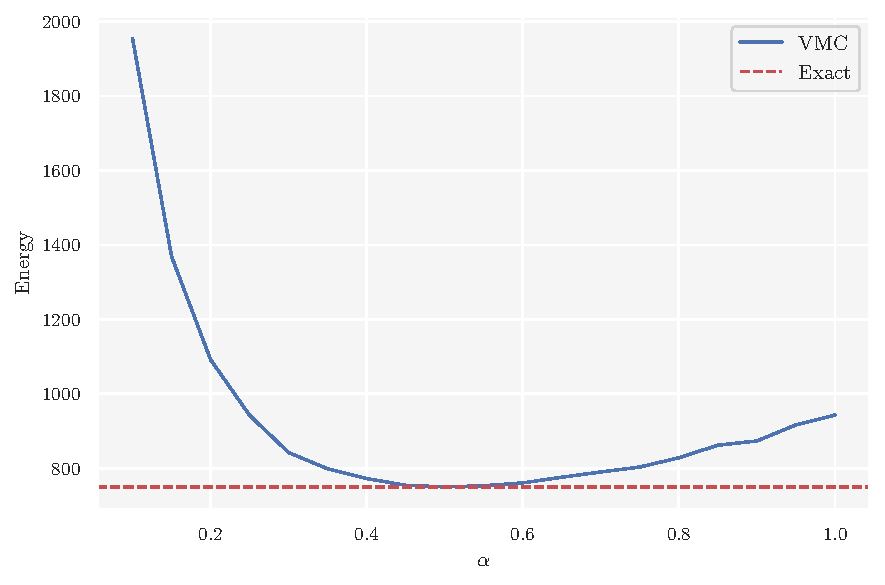
\includegraphics[scale=0.5]{latex/figures/grid_search_analytical.pdf}}}
\qquad
\subfloat[]{{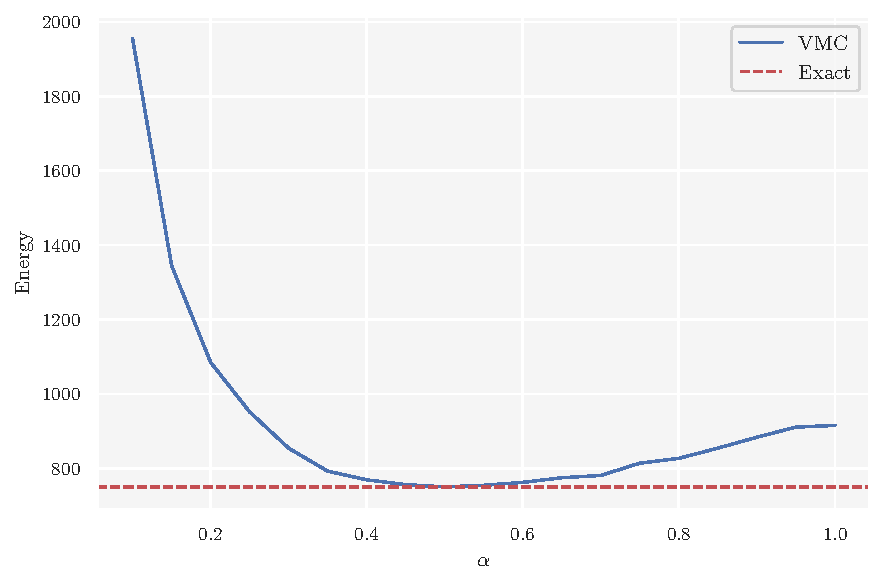
\includegraphics[scale=0.5]{latex/figures/grid_search_numerical.pdf}}}
\caption{Grid search $\alpha$, non-interacting system. \textbf{(a)} VMC computations with analytical expressions. \textbf{(b)} VMC computations with automatic differentiation.}
\label{fig:gridsearch}
\end{figure}



Discussion

%----------------------------------------------------------------
\subsubsection{Interacting}
%----------------------------------------------------------------

Compare log vs normal

%----------------------------------------------------------------
\subsection{Variational Energy}
%----------------------------------------------------------------

%----------------------------------------------------------------
\subsubsection{Non-Interacting}
%----------------------------------------------------------------

Discussion

\autoref{fig:non-interact_boxplot} shows 

\begin{figure}[!htb]
\centering
\subfloat[]{{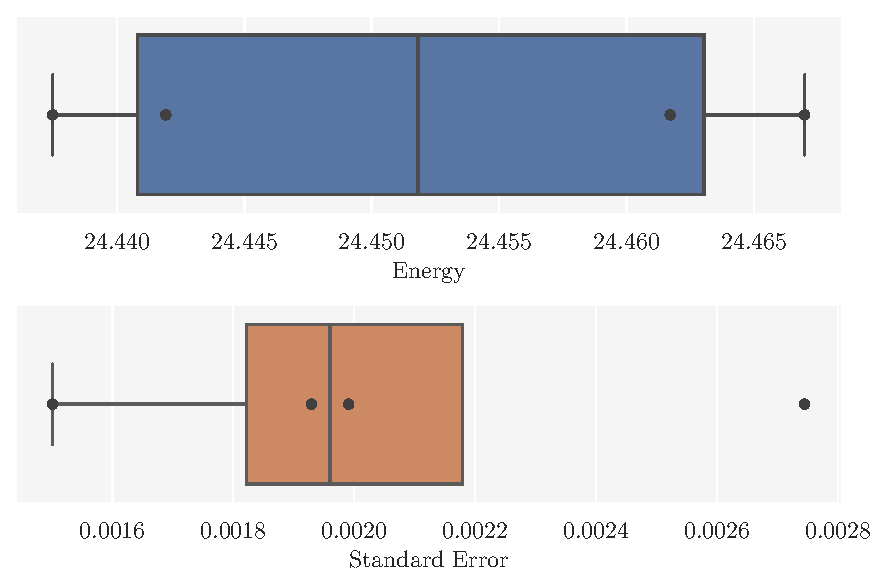
\includegraphics[scale=0.5]{latex/figures/boxplot_analytical_metropolis.pdf}}}
\qquad
\subfloat[]{{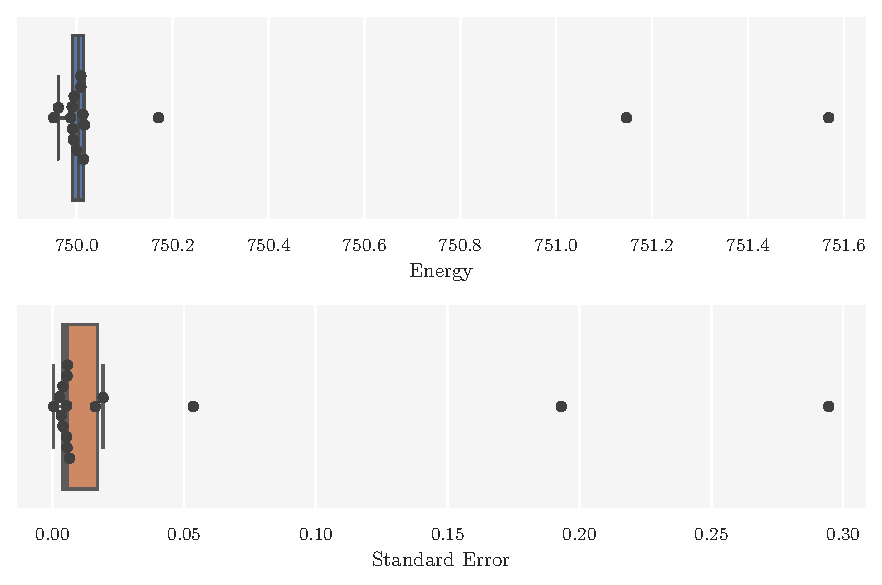
\includegraphics[scale=0.5]{latex/figures/boxplot_analytical_metropolis_hastings.pdf}}}
\qquad
\subfloat[]{{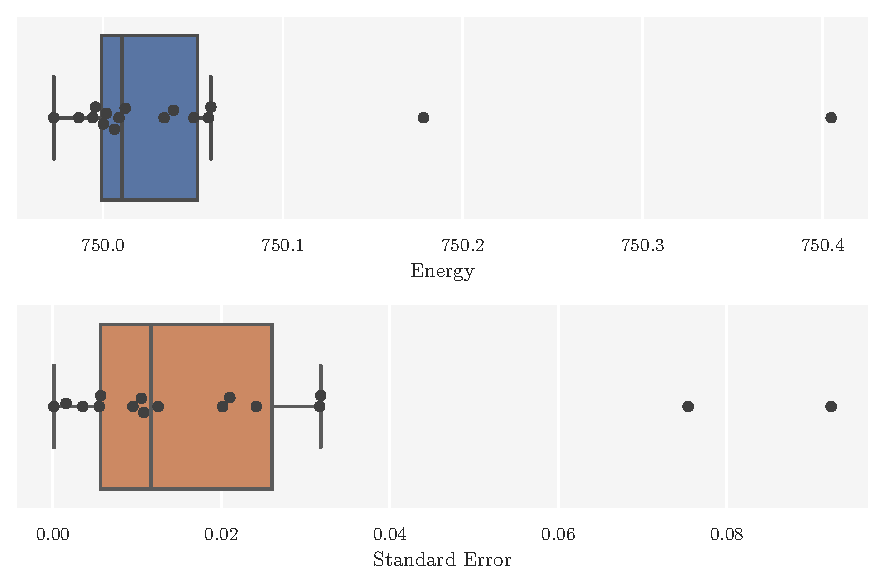
\includegraphics[scale=0.5]{latex/figures/boxplot_numerical_metropolis.pdf}}}
\qquad
\subfloat[]{{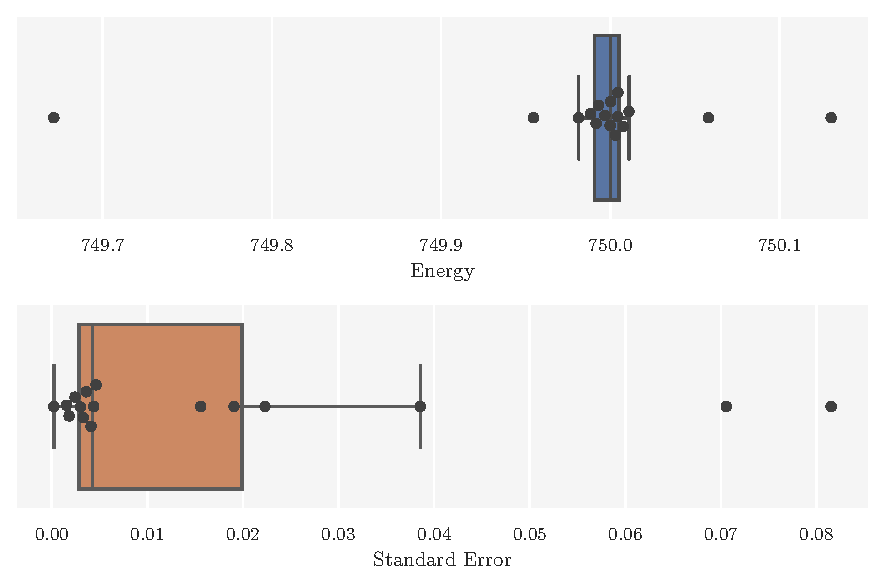
\includegraphics[scale=0.5]{latex/figures/boxplot_numerical_metropolis_hastings.pdf}}}
\caption{\textbf{(a)} Metropolis with analytical. \textbf{(b)} Metropolis-Hastings with analytical. \textbf{(c)} Metropolis with AD. \textbf{(d)} Metropolis-Hastings with AD.}
\label{fig:non-interact_boxplot}
\end{figure}

%----------------------------------------------------------------
\subsubsection{Interacting}
%----------------------------------------------------------------
\autoref{fig:interactions_plot} shows 
\begin{figure}[!htb]
\centering
\subfloat[]{{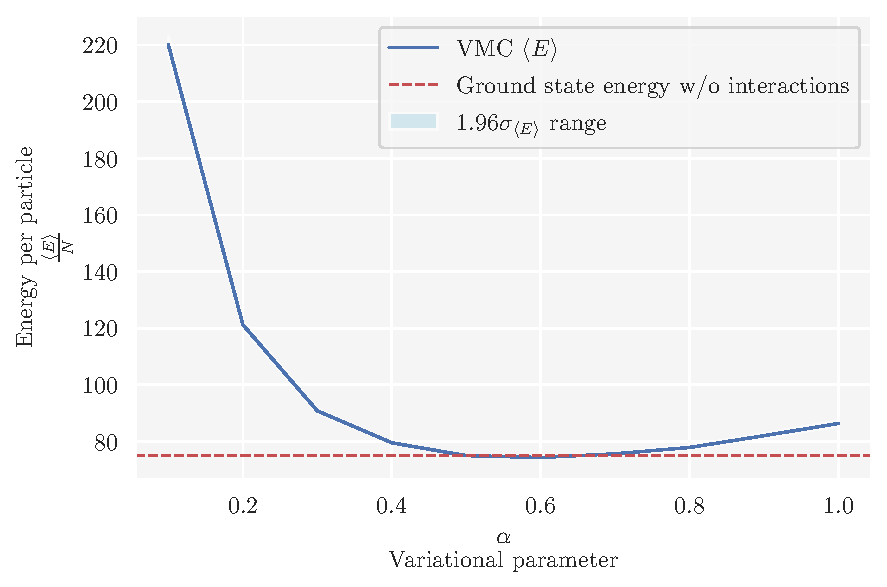
\includegraphics[scale=0.5]{latex/figures/grid_search_analytical_wo_interactions_N_50.pdf}}}
\qquad
\subfloat[]{{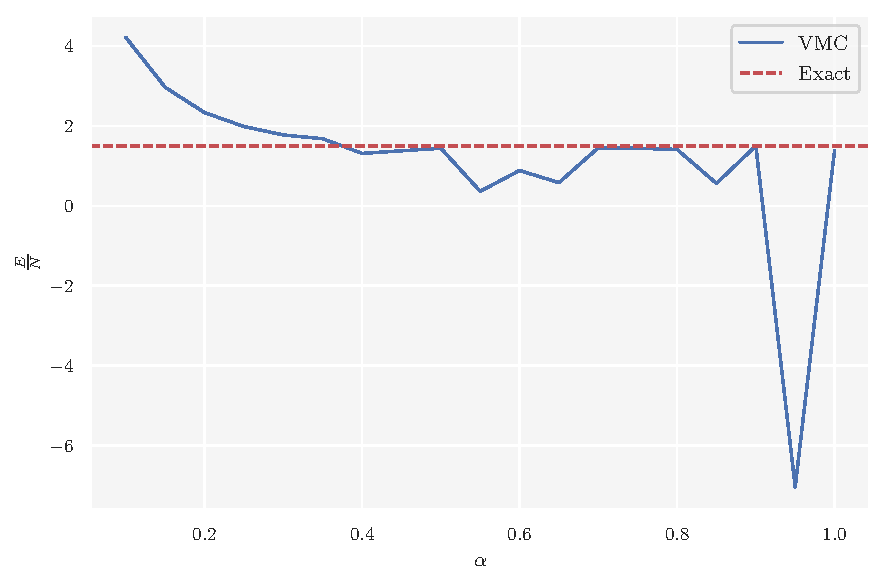
\includegraphics[scale=0.5]{latex/figures/grid_search_analytical_w_interactions_N_10.pdf}}}
\qquad
\subfloat[]{{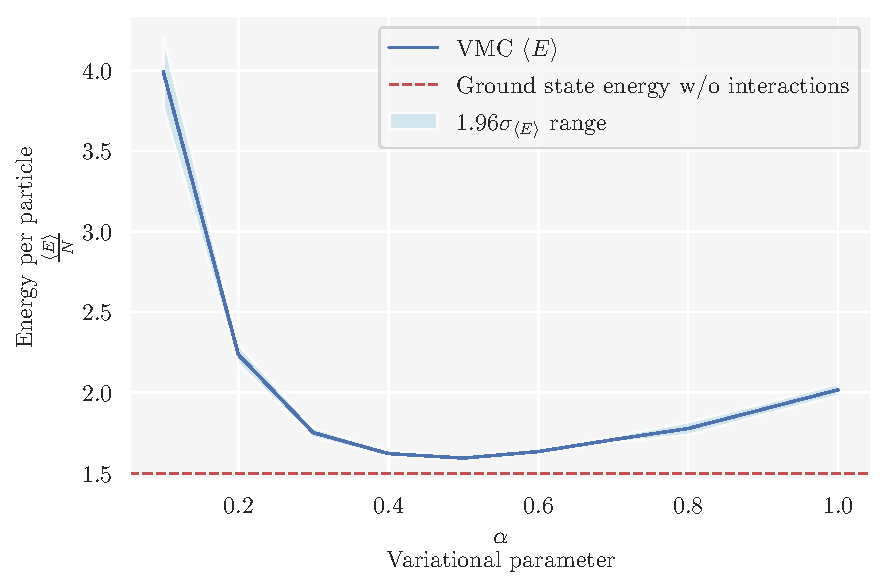
\includegraphics[scale=0.5]{latex/figures/grid_search_analytical_w_interactions_N_50.pdf}}}
\qquad
\subfloat[]{{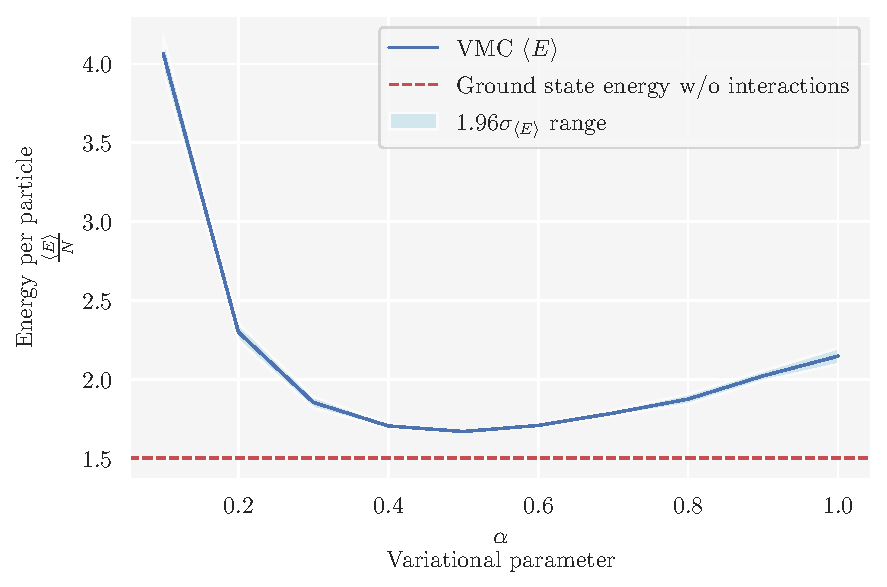
\includegraphics[scale=0.5]{latex/figures/grid_search_analytical_w_interactions_N_100.pdf}}}
\caption{\textbf{(a)} Metropolis with 50 non-interacting particles. \textbf{(b)} Metropolis with ten interacting particles. \textbf{(c)} Metropolis with 50 interacting particles. \textbf{(d)} Metropolis with 100 interacting particles.}
\label{fig:interactions_plot}
\end{figure}

\autoref{fig:comparisons_interactions_plot} shows 

\begin{figure}[H]
\begin{center}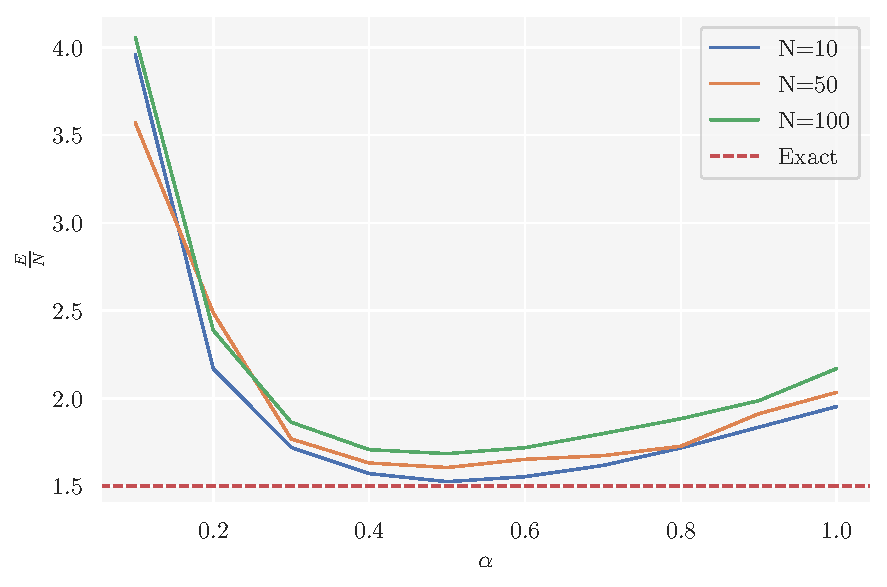
\includegraphics[scale=0.5]{latex/figures/grid_search_analytical_w_interactions_all_N.pdf}
\end{center}
\caption{Metropolis energy comparison between $N=10, 50, 100$ interacting particles, and $N=50$ non-interacting particles.}
\label{fig:comparisons_interactions_plot}
\end{figure}

\subsubsection{One-body densities}
\autoref{fig:one_body_densities} shows the sampled one body densities for $10$ and $100$ particles with interactions turned on and off. As the number of particles increases, the density of particles increases, and the interactions between the particles becomes a larger factor. For $10$ particles, the one body densities with and without interactions are almost identical. This means that for $10$ particles, the interactions do not have a large impact on the system. For $100$ particles, the radial one body densities for the interacting and non-interacting cases differ more. The particles in the interacting case are more spread out in the $2$-dimensional space than the non-interacting case. The interactions really do make a difference. 
\begin{figure}[H]
\centering
\subfloat[]{{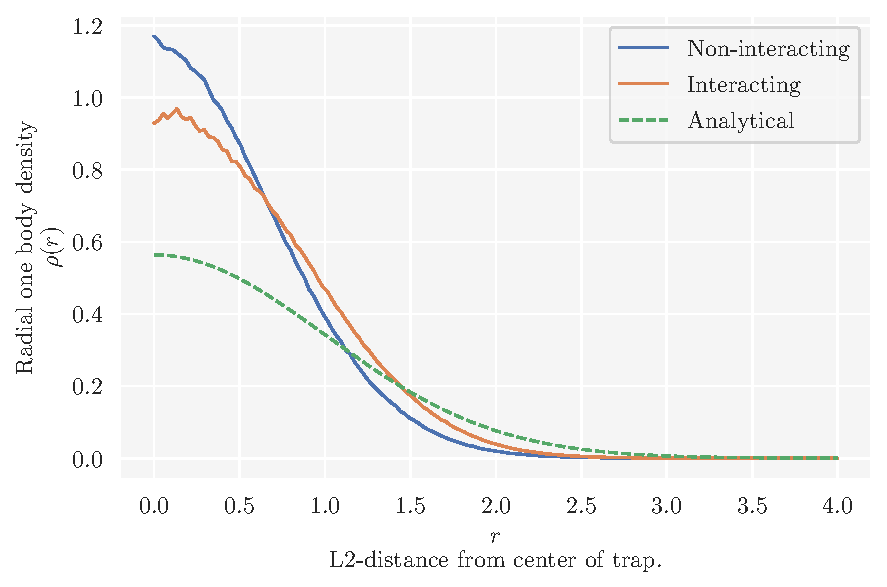
\includegraphics[scale=0.5]{latex/figures/OBD_N100.pdf}}}
\qquad
\subfloat[]{{\includegraphics[scale=0.5]{latex/figures/OBD_N100_scaled_with_volume.pdf}}}
\caption{\textbf{(a)} Comparison between the radial one body densities for $10$ particles with and without interactions (Jastrow factor $a=0.00433$) in $2$-dimensional space. \textbf{(b)} Comparison between the radial one body densities for $100$ particles with and without interactions (Jastrow factor $a=0.00433$) in $2$-dimensional space.}
\label{fig:one_body_densities}
\end{figure}
%\newpage
%%================================================================
\section{Discussion}\label{sec:Discussion}
%================================================================

%----------------------------------------------------------------
\subsection{Project Discussion 1}\label{sec:project discussion}
%----------------------------------------------------------------

%================================================================
\section{Conclusion}\label{sec:Conclusion}
%================================================================

Concluding, we observe that the statistical error using the RWM is larger than for LMH when there is an equal number of samples. In fact, we see that the statistical error in the sampling is very much lower. However, our implementation also depends on the convergence to the right $\alpha$, and the standard error of the mean of the energy samples in \autoref{fig:rwm_vs_lmh}
RWM is slow in terms of the total number of MC cycles, but each step is fast as it does not require gradients of the density. LMH on the other hand is faster in terms of the total number of MC cycles, but each step is slow as it uses gradients of the density at each step. Even taking the slowness of each step of LMH, it outperforms RWM. To achieve the same level of statistical error, the number of samples needed for the RWM would have to be much higher than the LMH. 
We found the analytical ground state of the non-interacting boson system to be $\frac{3}{2}\hbar\omega_0$ for the sperical trap, and $2.414215\hbar\omega_0$ for the elliptical trap. When the interactions simulated by the Jastrow correlation factor were included, we found an increase in the energy per particle proportional to the particle density. 

The one-body densities reveal that, when the bosons are interacting, the state of the system is dependent on the density of bosons in the trap. \autoref{fig:one_body_densities} shows that when the density is low, the interactions have a minor influence on the state of the system. One should think that when the interacting particles are close to one another, they interact with more frequency and strength, thus having a larger impact on the system state. If the interactions between the bosons are attractive, we therefore expect to observe a narrowing of the one-body density, and a spreading if the interactions were repulsive. We observe that the one-body density is more spread out in configuration space, which corresponds to a repellent potential, and an increase in the spread as a function of the density. 

Dette burde også med på en eller annen måte: The one-body densities reveal ...


(ref figure) demonstrates that LMH asymptotically mix considerably faster than RWM -> skal bety at den i prinsippet trenger færre MC cycles (men så er den dyrere i bruk da). 

\autoref{fig:rwm_vs_lmh} demonstrates that LMH asmptotically mix on
% Kan vi si noe om korrelasjon mellom samples LMH vs RWM? Blocking burde gi en pekepinn
% Hmm, sier du at korrelasjonen mellom dem går ned eller opp? Den skal vel i prinsippet gå opp i LMH, siden den ikke bare tar utgangspunkt i posisjonen ved forrige tidssteg, men også F(r), i kontrast til RWM som bare tar utgangspunkt i posisjonene ved forrige tidssteg? 

% Man vil helst ha ukorrelerte samples, og selvom LMH har flere deler som avhenger av forrige state er det ikke nødvendigvis slik at den genererer mer korrelerte samples. Men tror egentlig vi ikke har noen figur eller måling som viser dette tydelig, så det kan kanskje være noe å nevne for fremtidig research
% Okay, acceptance rate er mye høyere for LMH, så samples vil være mer ukorrelerte på grunn av det også. Et problem er at første figuren i appendiks viser egentlig at LMH er dårligere enn RWM til å estimere gradienten. Eller kanskje ikke dårligere, kanskje bare gradienten egentlig er så stor for alpha<0.5. 

% Et litt subtilt poeng som ikke kommer frem av den figuren er jo at den kun viser en statisisk trial. Kjører man den på nytt kunne figurene fort blitt reversert. Poenget med den er nok snarere at når det gjelder optimize har det ikke noe å si om man bruker RWM eller LMH, som også gir mening så lenge begge har optimal scale som leder den mot stationary state effektivt 

% Ah, ja, det er et godt poeng. Så det er 1 thread, ikke 16 per alpha. Okay. ja. Kom ikke så langt at jeg fikk skrevet det, men tolkningen av de er altså 1 stokastisk forsøk, men de viser jo en trend 

% Kunne evt laget en figur som viser hvordan det blir når alle starter på samme alpha

% På ett vis viser vi jo konvergens mot rette alpha? Ut fra figuren tror jeg nok at du har rett i at sammenlignen mellom RWM og LMH viser at når den stasjonære tilstanden er funnet, så er det hipp som happ hvilken vi velger? Jeg kan sette i gang en kjøring med 4 threads per alpha og plotte RWM mot LMH i samme plott, hvis du tenker det er lurt? Kan gjøre det med 16 nå. har skriptet mer eller mindre klart. Okay, jeg tenkte litt med hensyn på første linje i konklusjonen over her: Den erroren vi får er en større error i konvergens mot rett alpha enn det er i statistical error. Blir det feil? Skal se på det snart
%================================================================
\section{Future Work}\label{sec:Future}
%================================================================


%\section{Introduction}

A Bose-Einstein Condensate (BEC) is a gas composed of bosons, particles of integer spin that obey Bose-Einstein statistics, cooled down to critical temperature $T_C$ nearing absolute zero at which the gas goes through a phase transition. In this phase every particle falls into the lowest quantum state usually referred to as the ground state. Thus, every particle can be described by the same wave function and thus the expectation value of the energy is as follows

\begin{align}
    \left\langle E \right\rangle = \frac{\int d\mathbf{R} \mathbf{\Psi}_T^*(\mathbf{R},\alpha) H(\mathbf{R}) \mathbf{\Psi}_T(\mathbf{R},\alpha)}{\int d\mathbf{R} \mathbf{\Psi}_T^*(\mathbf{R},\alpha)\mathbf{\Psi}_T(\mathbf{R},\alpha)}
    \label{eq:energy-expectation-value}
\end{align}

where $\mathbf{R}$ is the vector containing the position of all particles and $\alpha$ is the variational parameter. The variational principle states that the expectation value $\left\langle E \right\rangle$ is an upper bound for the ground state energy $E_0$.

\begin{align}
    E_0 \leq \left\langle E \right\rangle
\end{align}

An example of a such system is Bose-Einstein Condensation (BEC) in gases of alkali atoms such as $^{87}$Rb, $^{23}$Na, $^{7}$Li confined in magnetic traps. These confined Bose systems are dilute, here we refer you to \cite{DuBois-Glyde01}. Where they calculated the  characteristic length of a typical trap for the $^{87}$Rb gas $a_{ho}$, the s-wave scattering length $a_{Rb}$ set to $100a_0$, where $a_0 = 0.5292 \text{ \AA}$ is the Bohr radius and the inner-atomic spacing $l \simeq 10^4 \text{ \AA}$. And giving that the  effective atom size is small compared to both the trap size and the inter-atomic spacing the system is indeed dilute. This alone means that the physics is dominated by the two-body collisions between particles, represented by the s-wave scattering length $a$. 

We will consider a system of $N$ bosons with mass $m$ which are trapped in a harmonic oscillator potential. Many theoretical studies of Bose-Einstein condensates in gases of alkali atoms confined in magnetic or optical traps have been conducted in the frame work of the Gross-Pitaevskii (GP) equation \cite{Fab-Polls99}. We will consider a system of $N$ bosons with mass $m$ which are trapped in a harmonic oscillator potential.

Typically large multi-dimensional systems like these are very complex and cannot be solved analytically, therefore we turn to numerical approaches in order to simulate the system. We'll start off by studying the non-interacting case where an analytical solution is presented and venture off to the correlated case, which you will see is extremely convoluted and can only be solved numerically. The analytical non-interacting case works as a validity gauge for our numerical approaches. We will be using Variational Monte Carlo (VMC) in order to arrive to a good estimate of what the ground state for \autoref{eq:energy-expectation-value} might be for any of the systems at hand. In addition we will be contrasting ordinary VMC to an importance sampling technique, utilizing the Fokker-Planck equation that takes educated guesses as to were the ground state might be as opposed to ordinary VMC.

\section{Theory}

\subsection{The System}

We're evaluating bosons trapped in a harmonic oscillator potential either spherical $(S)$ or elliptical $(E)$. The system itself generally consist of $N$ bosons with a fixed mass $m$ where they traverse along a $d$-dimensional room. Our generalized equations will mainly focus on the 3 dimensional case. The external potential $V_{ext}$ for both the spherical and the elliptical trap is given by

\begin{align}
    V_{ext} (\mathbf{r}) =
  \begin{cases}
    \frac{1}{2}m \omega_{ho}r^2 \ (S)\\
    \frac{1}{2}m \left[ \omega_{ho} \left( x^2+y^2 \right) + \omega_z^2 z^2 \right] \ (E)
  \end{cases}
  \label{eq:ext-pottential}
\end{align}

Where $\omega_{ho}$ defines the trap's potential strength and as for the elliptical case $\omega_{ho}$ is the frequency in the $xy$-plane or the perpendicular whilst $\omega_z$ is the frequency in the $z$-direction. At $T= 0\ K$ the mean amplitude of a single boson is given by $\left\langle x^2 \right\rangle = \left( \hbar/2m\omega_{ho} \right)$ such that $a_{ho}= \left( \hbar/m\omega_{ho} \right)^{1/2}$ defines the characteristic length of the trap. The ratio of the frequencies is denoted $\gamma = \omega_z/\omega_\perp$ leading to the ratio of the trap lengths $\left( a_\perp/a_z \right) = \left( \omega_z/\omega_\perp \right)^{1/2} = \sqrt{\gamma}$

The inter-boson interactions between two particles is expressed as a repulsive potential $V_{int}$ between the two. 

\begin{align}
    V_{int} (\mathbf{r}) =
  \begin{cases}
    \infty \text{ for } \abs{\mathbf{r}_i - \mathbf{r}_j} \leq a\\
    0 \text{ for } \abs{\mathbf{r}_i - \mathbf{r}_j} > a
  \end{cases}
  \label{eq:int-pottential}
\end{align}

Where a is the hard-core diameter of the bosons so $V_{int}$ naturally prevents the particles from ever occupying the same space in the case of a collision. The Hamiltonian for our harmonic oscillator trap, taking into account both of the potentials, is written as

\begin{align}
    H = \sum_i^N \left( \frac{-\hbar^2}{2m}\nabla^2_i + V_{ext}(\mathbf{r})  \right) + \sum_{i<j} V_{int}\left( \mathbf{r}_i, \mathbf{r}_j \right)
    \label{eq:Complete-Hamiltonian}
\end{align}

Where we have used the following convention for the inner potential:

\begin{align*}
    \sum_{i<j} V_{ij}= \sum_{i=1}^N \sum_{j=i+1}^N V_{ij}
    \intertext{Which is a double sum that runs over every pairwise interaction once.}
\end{align*}

For the $\sum_i^N$-part the first term is the kinetic energy of each particle and the second term is as previously mentioned the the external potential of the trap acting on each particle. The $\sum_{i<j}$-part is for the inter-boson interaction between a pair of particles.

Now that we laid the ground for the system, we are in need of one additional powerful tool that would describe the system in it's entirety throughout the whole process and that is a trial wave function. Our initial educated guess for the wave function consist of two parts one for the harmonic trap effecting every single particle each for it's own as seen in eq.$\ $\ref{eq:Complete-Hamiltonian} and one for the inner-boson interaction or in other words the correlated aspect of the system.

\begin{equation}
    \begin{split}
        \mathbf{\Psi}_T \left( \mathbf{r} \right) &= \mathbf{\Psi}_T \left( \mathbf{r}_1, \mathbf{r}_2, \mathbf{r}_3, \dots, \mathbf{r}_N, \alpha, \beta \right)\\ 
        &= \left[\prod_i g\left( \alpha, \beta, \mathbf{r}_i \right) \right] \left[ \prod_{j<k} f\left( a, \abs{r_j - r_k} \right) \right]
    \end{split}
    \label{eq:correlated-WF}
\end{equation}

where $\alpha$ and $\beta$ are two variational parameters and $a$ is diameter in eq.$\ $\ref{eq:int-pottential} for the hard-core \textit{shell} of the particle. The first term follows a Gaussian distribution and is a composition of the single-particle wave function $g$.

\begin{align}
    g\left( \alpha, \beta, \mathbf{r}_i \right) = e^{-\alpha\left(x_i^2 + y_i^2 +\beta z_i^2\right)}
    \label{eq:one-body-WF}
\end{align}

Here $\beta$ determines the elliptical shape of the distribution so in the case where $\beta = 1$ we end with a sphere and this indeed the case for the spherical trap. As for the correlation wave function $f$ also refered to as \textit{the Jastrow factor} and it's presented by

\begin{align}
    f\left( a, \abs{r_j - r_k} \right) = 
  \begin{cases}
    0\ &\abs{r_j - r_k} \geq a\\
    \left( 1 - \frac{a}{\abs{r_k - r_k}} \right)\ &\abs{r_j - r_k} > a
  \end{cases}
  \label{eq:Jastrow-WF}
\end{align}

\subsubsection{The Simple Gaussian}

For the non-interacting case eq. \ref{eq:Jastrow-WF} is a non-factor here so subsequently $f=1$. This is done by setting the hard-core diameter to $a= 0$ since in this case we are not interested in any boson-to-boson interaction and as such we get a product sequence over the Gaussian distribution for each particle. Furthermore to make so the trap follows a spherical form we set $\beta= 1$. From that we obtain the simplest form our wave function can take and it's given by

\begin{align}
    \mathbf{\Psi}_T \left( \mathbf{r}_1, \mathbf{r}_2, \mathbf{r}_3, \dots, \mathbf{r}_N, a= 0 , \beta = 1  \right)  = \prod_i e^{-\alpha r_i^2}
    \label{eq:Simple-Gaussian}
\end{align}

Will be referring  to eq. \ref{eq:Simple-Gaussian} as \textit{the simple Gaussian}. A quantity used in our Metropolis-Hastings optimization is the quantum force and for the Simple-Gaussian wave function it takes the form

\begin{align}
    F = 2\frac{\nabla \mathbf{\Psi}_T}{\mathbf{\Psi}_T} = -4\alpha\sum_i r_i
    \label{eq:quantum-force}
\end{align}

An entire derivation can be found in \textbf{\ref{sec:app} Appendix \ref{subsec:non-interacting}}.
 
\subsection{The Local Energy}

\begin{equation}
    E_L(\mathbf{r}) = \frac{1}{\mathbf{\Psi}_T (\mathbf{r})}H \mathbf{\Psi}_T (\mathbf{r})
    \label{eq:localenergy}
\end{equation}



\subsubsection{The Simple Gaussian Wave Function}

\textit{An entire walk-through of the calculation can be found in \textbf{\ref{sec:app}. Appendix \ref{subsec:non-interacting}.}} \\

For the Simple Gaussian case there's is no correlation and the Hamiltonian naturally becomes

\begin{align}
    H_{OB} = \sum_i^N \left( \frac{-\hbar^2}{2m}\nabla^2_i + V_{ext}(\mathbf{r})  \right)
    \label{eq:OB-Hamiltonian}
\end{align}

where OB stands for one-body. Since it's a spherical trap we use $(S)$ in eq. \ref{eq:ext-pottential}. We first start by determining an analytical solution for the Laplacian of the wave function from eq. \ref{eq:localenergy}.

\begin{align}
    \begin{split}
        \nabla_i^2 \mathbf{\Psi}_T (\mathbf{r}) &= \nabla_i \cdot \nabla_i \mathbf{\Psi}_T\\
        &= -2\alpha\nabla_i \cdot \left[x_i, y_i, z_i \right] \mathbf{\Psi}_T\\
        &= \left[ -2\alpha d + 4\alpha^2r_i^2 \right] \mathbf{\Psi}_T(\mathbf{r})
    \end{split}
\end{align}

where $d$ is the number of dimensions, case being $d=3$.

For the simple Gaussian trial function the local energy is given by

\begin{align}
    \begin{split}
        E_L(\mathbf{r}) &= \sum_i ^ N \left(-\frac{\hbar^2}{2m} \Big{[} -2\alpha d + 4\alpha^2 r_i^2 \Big{]} + V_{ext}(\mathbf{r}_i) \right) \\
        &= \sum_i ^ N \left(-\frac{\hbar^2}{2m} \Big{[} -2\alpha d + 4\alpha^2 r_i^2 \Big{]} +  \frac{1}{2}m\omega_{ho}r_i^2 \right) \\
        &= -\frac{\hbar^2}{2m}  \Big{[} -2\alpha Nd + 4\alpha^2 \sum_i ^ N r_i^2 \Big{]} +  \frac{1}{2}m\omega_{ho}\sum_i ^ N r_i^2
    \end{split}
    \label{eq:SG-local-energy}
\end{align}

As for our upcoming numerical analysis we will be using natural units instead of the physical constants, meaning $\hbar = m = \omega_{ho} =  1$, which yeilds

\begin{align}
    E_L(\mathbf{r}) &= \alpha Nd - 2\alpha^2\sum_{i=1}^N r_i^2 + \frac{1}{2}\omega^2_{ho}\sum_{i=1}^{N} r_i^2
\end{align}

For the case where $\omega_{ho}=1$ we find the ground state to occur for $\alpha = 0.5$

\begin{align}
    E_L(\mathbf{r}) &= \frac{Nd}{2}
    \label{eq:SG-ground-energy}
\end{align}

which will work as a gauge for the validity of our numerical solutions later on.

\subsubsection{The Full Wave Function}

\textit{An entire walk-through of the calculation can be found in \textbf{\ref{sec:app}. Appendix \ref{subsec:interacting}.}} \\

A more realistic case is the interacting case for bosons in an eliptical trap $(E)$ in eq. \ref{eq:ext-pottential}. Meaning we're looking at the correlated wave function eq. \ref{eq:correlated-WF}, where now $\beta$ could be different than $1$ and the hard-core diameter $a > 0$. This ultimately means that our wave function contains the Jastrow factor to govern the boson-to-boson interaction and the Hamiltonian contains the repulsive potential eq. \ref{eq:int-pottential}.

We rewrite the Jastrow factor as

\begin{align}
    f(r_{ij}) &= exp \left( \sum_{i<j}^N u \left( r_{ij} \right) \right)
    \intertext{here $r_{ij} = \abs{r_i - r_j}$ and $u(r_{ij}) = \ln f(r_{ij})$. In addition we express the one-boday part as}
    \phi(\mathbf{r}_i) &= g\left( \alpha, \beta, \mathbf{r}_i \right)
    \intertext{The final expression for the correlated wave function becomes}
    \mathbf{\Psi}_T \left( \mathbf{r} \right) &= \Bigg{[}\prod_i \phi(\mathbf{r}_i) \Bigg{]} \text{exp} \left( \sum_{i<j}^N u \left( r_{ij} \right) \right) 
\end{align}

It's the same as for the Simple Gaussian case we start by determining an analytical solution for the Laplacian then we can arrive to the Laplician-term in the local energy

\begin{align}
    \begin{split}
        \frac{1}{\mathbf{\Psi}_T}\nabla_k^2 \mathbf{\Psi}_T &= \frac{\nabla_k^2 \phi(\mathbf{r}_k)}{\phi(\mathbf{r}_k)} + 2\frac{\nabla_k \phi(\mathbf{r}_k)}{\phi(\mathbf{r}_k)} \sum_{l\neq k} u'(r_{kl})\frac{\Delta r_{kl}}{r_{kl}} \\
        &\qquad + \sum_{m\neq k} u'(r_{km})\frac{\Delta r_{km}}{r_{km}} \cdot \sum_{l\neq k} u'(r_{kl})\frac{\Delta r_{kl}}{r_{kl}} \\
        &\qquad + \sum_{l\neq k} u''(r_{kl}) + u'(r_{kl}) \frac{2}{r_{kl}}
    \end{split}
\end{align}

Where 

\begin{align}
    \frac{\nabla_k^2 \phi(\mathbf{r}_k)}{\phi(\mathbf{r}_k)} &= 4\alpha^2\mathbf{r}_k^2 -2\alpha(2 + \beta) \\
    \frac{\nabla_k \phi(\mathbf{r}_k)}{\phi(\mathbf{r}_k)} &= -2\alpha\mathbf{r}_k \\
    u'(r_{kl}) &= \frac{a}{r_{kl}\left( r_{kl} - a \right)} \\
    u''(r_{kl}) &= \frac{a^2 - 2a r_{kl}}{r_{kl}^2 (r_{kl}-a)^2}
\end{align}

The drift force is given by

\begin{align}
    F = 2\frac{\nabla \mathbf{\Psi}_T}{\mathbf{\Psi}_T} = \frac{\nabla_k \phi(\mathbf{r}_k)}{\phi (\mathbf{r}_k)} + \sum_{l\neq k} \nabla_k u(\mathbf{r}_{kl})
\end{align}

As already mentioned a complete walk-through for the gradient and the Laplacian can be found in the \textbf{Appendix}.

\subsubsection{Scaling the Hamiltonian}

\textit{An entire walk-through of the calculation can be found in \textbf{\ref{sec:app}. Appendix \ref{subsec:interacting}.}} \\

Since we are in the process of rewriting equations. Often quantum systems are expressed in units of $\hbar\omega$ for convenience. In the scaling for the Hamiltonian we aim to increase numerical stability by simplifying the expression for the tools we're working with and achieve a physical interpretation of the system by expressing the energy as units of $\hbar\omega$. This is done by factoring out $\hbar\omega_0$ and dividing the Hamiltonian by that factor, which yields

\begin{align}
    H = \frac{1}{2} \sum_i^N \left( -{\nabla}^2_i + {x}_i^2 + {y}_i^2 + \gamma^2 {z}_i^2  \right) + \sum_{i<j} V_{int}\left( \mathbf{r}_i, \mathbf{r}_j \right)
\end{align}

Following \textbf{\ref{sec:app}. Appendix \ref{subsec:interacting}.} we have used:

\begin{align}
    a_{h0} &= \sqrt{\hbar/m\omega_{ho}} = (1 - 2) \times 10^4\ \text{\AA}
    \intertext{as the length scale and where we defined the parameter}
    \gamma &= \omega_z/\omega_{ho}
    \intertext{Then scaled the particle coordinates and the hard-core diameter by $a_{h0}$, meaning}
    \mathbf{r'} &= \mathbf{r}/a_{ho} \implies \mathbf{r} = a_{ho}\mathbf{r'} \\
    a' &= a/a_{ho} \implies a = a_{ho}a'
\end{align}

The hard-core diameter for the bosons was fixed to $a/a_{ho} = 0.00433$ and $\beta = \gamma = \sqrt{8} \approx 2.82843$ similar to what was done in \cite{MJensen05} and \cite{DuBois-Glyde01}

\twocolumn[
    \begin{@twocolumnfalse}
        \section{Appendix}
        \label{sec:app}
        \subsection{Calculations for non-interacting bosons}
        \label{subsec:non-interacting}
        \begin{align*}
            E_L(\mathbf{r}) &= \frac{1}{\mathbf{\Psi}_T (\mathbf{r})} H \mathbf{\Psi}_T (\mathbf{r}) \\
            &= \frac{1}{\mathbf{\Psi}_T (\mathbf{r})} \Bigg{[}\sum_i ^ N \left(-\frac{\hbar^2}{2m} \nabla^2_i + V_{ext}(\mathbf{r}_i) \right) \Bigg{]}\mathbf{\Psi}_T (\mathbf{r})
        \end{align*}
        Starting with the $H \mathbf{\Psi}_T (\mathbf{r})$ part of the equation
        \begin{align}
            \begin{split}
                H \mathbf{\Psi}_T (\mathbf{r}) &= \Bigg{[}\sum_i ^ N \left(-\frac{\hbar^2}{2m} \nabla^2_i + V_{ext}(\mathbf{r}_i) \right) \Bigg{]} \mathbf{\Psi}_T (\mathbf{r})\\
                &= \sum_i ^ N \left(-\frac{\hbar^2}{2m} \nabla^2_i \mathbf{\Psi}_T (\mathbf{r}) + V_{ext}(\mathbf{r}_i) \mathbf{\Psi}_T (\mathbf{r}) \right)
            \end{split}
            \intertext{Solving $\sum_i ^ N - \frac{\hbar^2}{2m} \nabla^2_i \mathbf{\Psi}_T$, the sum over $i$ for the Laplacian makes it so we compute the second derivative of the wave function with respect to each particle, for a particle $k$ the second derivatives is expressed as}
            &\nabla^2_k \prod_i e^{-\alpha |\mathbf{r}_i|^2}= \nabla^2_k \prod_i e^{-\alpha r_i^2}\\
            \intertext{where $k$ is an element in $\sum_i^N$.}
            \prod_{i \neq k} e^{-\alpha |\mathbf{r}_i|^2}\nabla^2_k e^{-\alpha |\mathbf{r}_k|^2} &= \prod_{i \neq k} e^{-\alpha |\mathbf{r}_i|^2}\nabla^2_k e^{-\alpha \left(x_k^2 + y_k^2 + z_k^2 \right)}
            \intertext{We start by finding the general expression for the gradient ($\nabla$)}
            \begin{split}
                \nabla_k e^{-\alpha \left(x_k^2 + y_k^2 + z_k^2 \right)}&= \Bigg{[}\frac{\partial}{\partial x}, \frac{\partial}{\partial y}, \frac{\partial}{\partial z}\Bigg{]}e^{-\alpha \left(x_k^2 + y_k^2 + z_k^2 \right)}\\
                &= \bigg{[}-2\alpha x_k e^{-\alpha|\mathbf{r}_k|^2}, -2\alpha y_k e^{-\alpha|\mathbf{r}_k|^2}, -2\alpha z_k e^{-\alpha|\mathbf{r}_k|^2} \bigg{]}\\
                &= -2\alpha \Big{[} x_k, y_k, z_k \Big{]} e^{-\alpha|\mathbf{r}_k|^2} = -2\alpha\mathbf{r}_k e^{-\alpha|\mathbf{r}_k|^2}
            \end{split}
            \intertext{Bringing back the product sequence we get}
            \prod_{i \neq k} e^{-\alpha |\mathbf{r}_i|^2}\nabla_k e^{-\alpha |\mathbf{r}_k|^2} &=  -2\alpha\mathbf{r}_k \mathbf{\Psi}_T (\mathbf{r})
            \intertext{Now for the Laplacian ($\nabla^2$)}
            \begin{split}
                \nabla^2_k e^{-\alpha|\mathbf{r}_k|^2}&= -2\alpha\nabla_k\mathbf{r}_k e^{-\alpha|\mathbf{r}_k|^2} = -2\alpha \Bigg{[}\frac{\partial}{\partial x}, \frac{\partial}{\partial y}, \frac{\partial}{\partial z}\Bigg{]} \Big{[} x_k, y_k, z_k \Big{]} e^{-\alpha|\mathbf{r}_k|^2}\\
                &= -2\alpha \frac{\partial}{\partial x} x_k e^{-\alpha|\mathbf{r}_k|^2} -2\alpha \frac{\partial}{\partial y} y_k e^{-\alpha|\mathbf{r}_k|^2} -2\alpha \frac{\partial}{\partial z} z_k e^{-\alpha|\mathbf{r}_k|^2}\\
                & \begin{matrix}
                    = & -2\alpha \left( e^{-\alpha|\mathbf{r}_k|^2} - 2\alpha x_k^2 e^{-\alpha|\mathbf{r}_k|^2} \right)\\
                    & -2\alpha \left(e^{-\alpha|\mathbf{r}_k|^2} - 2\alpha y_k^2e^{-\alpha|\mathbf{r}_k|^2} \right)\\
                    & -2\alpha \left( e^{-\alpha|\mathbf{r}_k|^2} - 2\alpha z_k^2 e^{-\alpha|\mathbf{r}_k|^2} \right)
                \end{matrix}\\
                &= -2\alpha \bigg{[} \left( 1 - 2\alpha x_k^2  \right) + \left( 1 - 2\alpha y_k^2  \right) + \left( 1 - 2\alpha z_k^2  \right) \bigg{]} e^{-\alpha|\mathbf{r}_k|^2}\\
                &= -2\alpha \Big{[} 3 - 2\alpha |\mathbf{r}_k|^2 \Big{]} e^{-\alpha|\mathbf{r}_k|^2}
            \end{split}
            \intertext{for a general $d$-dimensional case our expression then becomes}
            &= -2\alpha \Big{[} d - 2\alpha |\mathbf{r}_k|^2 \Big{]}  e^{-\alpha|\mathbf{r}_k|^2} = \Big{[} -2\alpha d + 4\alpha^2 r_k^2 \Big{]} e^{-\alpha|\mathbf{r}_k|^2}
        \end{align}
    \end{@twocolumnfalse}
]


\twocolumn[
    \begin{@twocolumnfalse}
        \begin{align}
            \intertext{ where $d$ is the number of dimension, 3 in our case. Bringing back the product sequence we get}
            \prod_{i \neq k} e^{-\alpha |\mathbf{r}_i|^2}\Big{[} -2\alpha d + 4\alpha^2 r_k^2 \Big{]} e^{-\alpha|\mathbf{r}_k|^2} &= \Big{[} -2\alpha d + 4\alpha^2 r_k^2 \Big{]} \mathbf{\Psi}_T (\mathbf{r})
            \intertext{The final analytical expression for $H \mathbf{\Psi}_T (\mathbf{r})$ is}
            \begin{split}
                H \mathbf{\Psi}_T (\mathbf{r}) &= \sum_i ^ N \left(-\frac{\hbar^2}{2m} \nabla^2_i \mathbf{\Psi}_T (\mathbf{r}) + V_{ext}(\mathbf{r}_i) \mathbf{\Psi}_T (\mathbf{r}) \right)\\
                &= \sum_i ^ N \left(-\frac{\hbar^2}{2m} \Big{[} -2\alpha d + 4\alpha^2 r_i^2 \Big{]} \mathbf{\Psi_T}(\mathbf{r}) + V_{ext}(\mathbf{r}_i) \mathbf{\Psi}_T (\mathbf{r}) \right)\\
                &= \sum_i ^ N \left(-\frac{\hbar^2}{2m} \Big{[} -2\alpha d + 4\alpha^2 r_i^2 \Big{]} + V_{ext}(\mathbf{r}_i) \right) \mathbf{\Psi}_T (\mathbf{r})
            \end{split}
            \intertext{Using what we've obtained, the final expression for the local energy is then}
            \begin{split}
                E_L(\mathbf{r}) &= \frac{1}{\mathbf{\Psi}_T (\mathbf{r})} H \mathbf{\Psi}_T (\mathbf{r}) \\
                &= \frac{1}{\mathbf{\Psi}_T (\mathbf{r})} \Bigg{[} \sum_i ^ N \left(-\frac{\hbar^2}{2m} \Big{[} -2\alpha d + 4\alpha^2 r_i^2 \Big{]} + V_{ext}(\mathbf{r}_i) \right)\Bigg{]} \mathbf{\Psi}_T (\mathbf{r})\\
                &= \sum_i ^ N \left(-\frac{\hbar^2}{2m} \Big{[} -2\alpha d + 4\alpha^2 r_i^2 \Big{]} + V_{ext}(\mathbf{r}_i) \right)
            \end{split}
        \end{align}
        
    For the case of a spherical potential with $\beta = 1$, $\omega_{ho} = 1$
        
        \begin{align}
            \begin{split}
                E_L(\mathbf{r}) &= \sum_{i=1}^N \left( -\frac{\hbar^2}{2m} \Bigg{[} -2\alpha d + 4\alpha^2r_i^2 \Bigg{]}+ \frac{1}{2}m\omega_{ho}^2r_i^2 \right)\\
                &= \frac{-h^2}{2m} \Bigg{[} -2\alpha Nd + 4\alpha^2 \sum_{i=1}^N r_i^2\Bigg{]} + \frac{1}{2}m\omega_{ho}^2 \sum_{i=1}^N r_i^2
            \end{split}
                \intertext{If we were to work with natural units, meaning $\hbar = m = 1$}
            \begin{split}
                &= \frac{-1}{2} \Bigg{[} -2\alpha Nd + 4\alpha^2 \sum_{i=1}^N r_i^2\Bigg{]} + \frac{1}{2}\omega_{ho}^2 \sum_{i=1}^N r_i^2\\
                &= \alpha Nd - 2\alpha^2 \sum_{i=1}^N r_i^2 + \frac{1}{2}\omega_{ho}^2 \sum_{i=1}^N r_i^2
            \end{split}
                \intertext{Choosing to set the oscillator frequency $\omega_{ho} = 1$ the ground state occurs for $\alpha = 0.5$. Which in turn yields a simple analytical expression}
            \begin{split}
                &= \frac{1}{2} Nd - \frac{1}{2} \sum_{i=1}^N r_i^2 + \frac{1}{2} \sum_{i=1}^N r_i^2 = \frac{Nd}{2}
            \end{split}
        \end{align}
        which we would use to test our numerical solution for the Hamiltonian. \\

        Finding an analytical expression for the drift force

        \begin{align}
            \begin{split}
                F &= \frac{2\nabla \mathbf{\Psi}_T}{\mathbf{\Psi}_T}\\
                \nabla \mathbf{\Psi}_T&= \sum_i \nabla_i \mathbf{\Psi}_T= -2\alpha \sum_i \mathbf{r}_i \mathbf{\Psi}_T\\
                F &= \frac{-4\alpha \sum_i \mathbf{r}_i \mathbf{\Psi}_T}{\mathbf{\Psi}_T} = -4\alpha \sum_i \mathbf{r}_i\\
                F_k &= -4\alpha \mathbf{r}_k
            \end{split}
        \end{align}
    \end{@twocolumnfalse}
]


\twocolumn[
    \begin{@twocolumnfalse}
        Finding an expression for the numerical second derivative. We start with the second-order central derivative
        
        \begin{align}
            f''(x) = \frac{f(x+h) - 2f(x) + f(x-h)}{h^2}
        \end{align}
        
        Wave function second derivative
        \begin{align}
            \nabla^2 \mathbf{\Psi}_T(\mathbf{r}) &= \sum_i^N \nabla_i^2 \mathbf{\Psi}_T(\mathbf{r})
            \intertext{for a particle $k$ in a 3 dimensional case}
            \prod_{i \neq k} e^{-\alpha |\mathbf{r}_i|^2}\nabla^2_k e^{-\alpha |\mathbf{r}_k|^2} &= \prod_{i \neq k} e^{-\alpha |\mathbf{r}_i|^2} \left(\frac{\partial^2}{\partial x_k^2} + \frac{\partial^2}{\partial y_k^2} + \frac{\partial^2}{\partial z_k^2}\right) e^{-\alpha \left(x_k^2 + y_k^2 + z_k^2 \right)}
        \end{align}

        \begin{align}
            \frac{\partial^2}{\partial x_k^2} e^{-\alpha \left(x_k^2 + y_k^2 + z_k^2 \right)} &= \frac{e^{-\alpha \left((x_k+h)^2 + y_k^2 + z_k^2 \right)} - 2e^{-\alpha \left(x_k^2 + y_k^2 + z_k^2 \right)} + e^{-\alpha \left((x_k-h)^2 + y_k^2 + z_k^2 \right)}}{h^2}
        \end{align}

        \begin{align}
            \begin{split}
                \left(\frac{\partial^2}{\partial x_k^2} + \frac{\partial^2}{\partial y_k^2} + \frac{\partial^2}{\partial z_k^2}\right) \! e^{-\alpha \left(x_k^2 + y_k^2 + z_k^2 \right)} \! =
                \frac{- 2\cdot 3 e^{-\alpha \left(x_k^2 + y_k^2 + z_k^2 \right)}}{h^2} & + \! \left(exp\left((x_k+h)^2\right) + exp\left((x_k-h)^2\right)\right)/h^2 \\
                & + \! \left(exp\left((y_k+h)^2\right) + exp\left((y_k-h)^2\right)\right)/h^2 \\
                & + \! \left(exp\left((z_k+h)^2\right) + exp\left((z_k-h)^2\right)\right)/h^2
            \end{split}
        \end{align}

        \begin{align}
            \begin{split}
                \prod_{i \neq k} e^{-\alpha |\mathbf{r}_i|^2}\nabla^2_k e^{-\alpha |\mathbf{r}_k|^2} = \frac{- 2\cdot 3 \mathbf{\Psi}_T(\mathbf{r})}{h^2} + \! \prod_{i \neq k} e^{-\alpha |\mathbf{r}_i|^2} &\Bigg{[} \left(exp\left((x_k+h)^2\right) + exp\left((x_k-h)^2\right)\right)/h^2 \\
                & + \! \left(exp\left((y_k+h)^2\right) + exp\left((y_k-h)^2\right)\right)/h^2 \\
                & + \! \left(exp\left((z_k+h)^2\right) + exp\left((z_k-h)^2\right)\right)/h^2 \Bigg{]}
            \end{split}
        \end{align}
        
        \textbf{Not the best notation but I had to make lemonades out of \LaTeX! \\}
        
        For a $d$-dimensional case
        
        \begin{align}
            \begin{split}
                \prod_{i \neq k} e^{-\alpha |\mathbf{r}_i|^2}\nabla^2_k e^{-\alpha |\mathbf{r}_k|^2} = \frac{- 2\cdot d \mathbf{\Psi}_T(\mathbf{r})}{h^2} + \! \prod_{i \neq k} e^{-\alpha |\mathbf{r}_i|^2} &\bigg{[} \left(exp\left((x_k+h)^2\right) + exp\left((x_k-h)^2\right)\right)/h^2 \\
                & + \! \left(exp\left((y_k+h)^2\right) + exp\left((y_k-h)^2\right)\right)/h^2 \\
                & + \! \left(exp\left((z_k+h)^2\right) + exp\left((z_k-h)^2\right)\right)/h^2 \bigg{]}
            \end{split}
        \end{align}
        
        Setting up for Gradient descent:

        \begin{align}
            \begin{split}
                \bar{\mathbf{\Psi}}_T &= \frac{d\mathbf{\Psi}_T}{d\alpha} = \frac{d }{d\alpha} \prod_{i} e^{-\alpha r_i^2} = \frac{d }{d\alpha} e^{-\alpha\sum_i r_i^2} = -\sum_i r_i^2 \cdot e^{-\alpha \sum_i r_i^2}\\
                \frac{\bar{\mathbf{\Psi}}_T}{\bar{\mathbf{\Psi}}_T} &= \frac{-\sum_i r_i^2 \cdot e^{-\alpha \sum_i r_i^2}}{e^{-\alpha\sum_i r_i^2}} = -\sum_i r_i^2
            \end{split}
        \end{align}
    \end{@twocolumnfalse}
]

\twocolumn[
    \begin{@twocolumnfalse}
        \subsection{Calculations for interacting bosons}
        \label{subsec:interacting}
        \subsubsection{Scaling the Hamiltonian}
         \begin{align}
             H &= \sum_i^N \left( \frac{-\hbar^2}{2m}\nabla^2_i + V_{ext}(\mathbf{r})  \right) + \sum_{i<j} V_{int}\left( \mathbf{r}_i, \mathbf{r}_j \right) \\
             &= \sum_i^N \left( \frac{-\hbar^2}{2m}\nabla^2_i + \frac{1}{2} m\Big{[} \omega_{ho}^2\left( x_i^2 + y_i^2 \right) + \omega_z^2 z_i^2 \Big{]}  \right) + \sum_{i<j} V_{int}\left( \mathbf{r}_i, \mathbf{r}_j \right) 
             \intertext{For convenience we want to express the energy in units of $\hbar\omega$. Therefor we introduce a scaling factor $\hbar\omega_{ho}$}
             &= \frac{\hbar\omega_{ho}}{2} \sum_i^N \left( -\frac{\hbar}{m\omega_{ho}}\nabla^2_i +  \frac{m \omega_{ho}}{\hbar}\Bigg{[} x_i^2 + y_i^2 + \frac{\omega_z^2}{\omega_{ho}^2} z_i^2 \Bigg{]}  \right) + \sum_{i<j} V_{int}\left( \mathbf{r}_i, \mathbf{r}_j \right)
             \intertext{Inspecting the $\hbar/m\omega_{ho}$-factor we find that its physical SI unit is $m$. So naturally this our length scale and we define it as}
             a_{ho} &= \sqrt{\hbar/m\omega_{ho}}
             \intertext{which helps shape up the scaled lengths}
             \mathbf{r'} &= \mathbf{r}/a_{ho} \implies \mathbf{r} = a_{ho}\mathbf{r'} \\
             a' &= a/a_{ho} \implies a = a_{ho}a'
             \intertext{and naturally the Laplacian becomes}
             {\nabla'}_i^2 &= a_{ho}^2\nabla_i^2 \implies \nabla_i^2 = \frac{{\nabla'}_i^2}{a_{ho}^2}
             \intertext{We also define the parameter}
             \gamma &= \omega_z/\omega_{ho}
             \intertext{Dividing the Hamiltonian by the scaling factor $\hbar\omega_{ho}$, yields}
             &= \frac{1}{2} \sum_i^N \left( -a_{ho}^2\nabla^2_i +  a_{ho}^{-2}\Bigg{[} x_i^2 + y_i^2 + \gamma^2 z_i^2 \Bigg{]}  \right) + \sum_{i<j} V_{int}\left( \mathbf{r}_i, \mathbf{r}_j \right) \\
             \intertext{then scaling the Hamiltonian}
             &= \frac{1}{2} \sum_i^N \left( -{\nabla'}^2_i + {x'}_i^2 + {y'}_i^2 + \gamma^2 {z'}_i^2  \right) + \sum_{i<j} V_{int}\left( \mathbf{r}_i, \mathbf{r}_j \right)
         \end{align}
    \end{@twocolumnfalse}
]

\twocolumn[
    \begin{@twocolumnfalse}
        \subsubsection{The Local Energy}
        \begin{align*}
            E_L(\mathbf{r}) &= \frac{1}{\mathbf{\Psi}_T (\mathbf{r})} H \mathbf{\Psi}_T (\mathbf{r}) \\
            H &= \sum_i^N \left( \frac{-\hbar^2}{2m}\nabla^2_i + V_{ext}(\mathbf{r})  \right) + \sum_{i<j} V_{int}\left( \mathbf{r}_i, \mathbf{r}_j \right)
        \end{align*}
        We start by rewriting eq. \ref{eq:correlated-WF} as
        \begin{align}
            \begin{split}
                \mathbf{\Psi}_T \left( \mathbf{r} \right) &= \Bigg{[}\prod_i \phi(\mathbf{r}_i) \Bigg{]} \text{exp} \left( \sum_{i<j}^N u \left( r_{ij} \right) \right)
                \label{eq:correlated-WF-App}
            \end{split}
            \intertext{where $r_{ij} = \abs{r_i - r_j}$ and where we have rewritten the one-body part}
            \begin{split}
                g\left( \alpha, \beta, \mathbf{r}_i \right) = \phi(\mathbf{r}_i)
            \end{split}
            \intertext{and the Jastrow factor}
            \begin{split}
                f(r_{ij}) &= exp \left( \sum_{i<j}^N u \left( r_{ij} \right) \right)
            \end{split}
        \end{align}
        for $u$ is defined as $u(r_{ij}) = \ln f(r_{ij})$. To keep things tidy we define $\Psi_{OB}$ to be the one body-part and $\Psi_C$ to be the correlated part of eq. \ref{eq:correlated-WF-App}. The gradient $\nabla_k$ of a particle $k$ can be found by solving
        \begin{align}
            \nabla_k \Psi_T &= \Psi_C \nabla_k \Psi_{OB} + \Psi_{OB}\nabla_k \Psi_C \\
            \nabla_k \Psi_{OB} &= \nabla_k \prod_i \phi(\mathbf{r}_i)  = \nabla_k \phi(\mathbf{r}_k)\prod_{i\neq k} \phi(\mathbf{r}_i) \\
            \nabla_k \Psi_C &= \nabla_k \text{exp} \left( \sum_{i<j}^N u \left( r_{ij} \right) \right) = \text{exp} \left( \sum_{i<j}^N u \left( r_{ij} \right) \right) \sum_{l\neq k} \nabla_k u(r_{kl})
        \end{align}
        Where we've used the fact that all the terms $r_{ij}$ that don't contain the position $r_k$ of particle $k$ are zero and we're left with $r_k$ dependent terms. Thus, the first derivative can now be expressed as
        \begin{align}
            \nabla_k \Psi_T &= \text{exp} \left( \sum_{i<j}^N u \left( r_{ij} \right) \right) \cdot \nabla_k \phi(\mathbf{r}_k) \prod_{i\neq k} \phi(\mathbf{r}_i) + \prod_i \phi(\mathbf{r}_i)  \cdot \text{exp} \left( \sum_{i<j}^N u \left( r_{ij} \right) \right) \sum_{l\neq k} \nabla_k u(r_{kl})
        \end{align}
        The Laplacian
        \begin{align}
            \begin{split}
                \nabla_k^2 \Psi_T = \nabla_k \Bigg{[} \text{exp} \left( \sum_{i<j}^N u \left( r_{ij} \right) \right) \cdot \prod_{i\neq k} \phi(\mathbf{r}_i) \nabla_k \phi(\mathbf{r}_k) + \prod_i \phi(\mathbf{r}_i)  \cdot \text{exp} \left( \sum_{i<j}^N u \left( r_{ij} \right) \right) \sum_{l\neq k} \nabla_k u(r_{kl}) \Bigg{]}
            \end{split}
            \intertext{Starting with the first term}
            \begin{split}
                \nabla_k \Bigg{[} \text{exp} \left( \sum_{i<j}^N u \left( r_{ij} \right) \right) \cdot \prod_{i\neq k} \phi(\mathbf{r}_i) \nabla_k \phi(\mathbf{r}_k) \Bigg{]} = \nabla_k^2 \phi(\mathbf{r}_k) \prod_{i\neq k} \phi(\mathbf{r}_i) &\cdot \text{exp} \left( \sum_{i<j}^N u \left( r_{ij} \right) \right) \\
                & + \nabla_k \phi(\mathbf{r}_k) \prod_{i\neq k} \phi(\mathbf{r}_i) \cdot \nabla_k \text{exp} \left( \sum_{i<j}^N u \left( r_{ij} \right) \right) \\
            \end{split}
        \end{align}
    \end{@twocolumnfalse}
]

\twocolumn[
    \begin{@twocolumnfalse}
        \begin{align}
            &= \nabla_k^2 \phi(\mathbf{r}_k) \prod_{i\neq k} \phi(\mathbf{r}_i) \cdot \text{exp} \left( \sum_{i<j}^N u \left( r_{ij} \right) \right) + \nabla_k \phi(\mathbf{r}_k) \prod_{i\neq k} \phi(\mathbf{r}_i) \cdot \text{exp} \left( \sum_{i<j}^N u \left( r_{ij} \right) \right) \sum_{l\neq k} \nabla_k u(r_{kl})
        \end{align}
        Now for the second term
        \begin{align}
            \begin{split}
                \nabla_k \Bigg{[} \prod_i \phi(\mathbf{r}_i) \cdot \text{exp} \left( \sum_{i<j}^N u \left( r_{ij} \right) \right) \sum_{l\neq k} \nabla_k u(r_{kl}) \Bigg{]} &= \nabla_k \prod_i \phi(\mathbf{r}_i) \cdot \text{exp} \left( \sum_{i<j}^N u \left( r_{ij} \right) \right) \sum_{l\neq k} \nabla_k u(r_{kl}) \\
                &\qquad + \prod_i \phi(\mathbf{r}_i)  \cdot \nabla_k \text{exp} \left( \sum_{i<j}^N u \left( r_{ij} \right) \right) \sum_{l\neq k} \nabla_k u(r_{kl}) \\
                &\qquad + \prod_i \phi(\mathbf{r}_i)  \cdot \text{exp} \left( \sum_{i<j}^N u \left( r_{ij} \right) \right) \nabla_k \sum_{l\neq k} \nabla_k u(r_{kl}) \\
                &= \prod_{i\neq k} \phi(\mathbf{r}_i) \nabla_k \phi(\mathbf{r}_k) \cdot \text{exp} \left( \sum_{i<j}^N u \left( r_{ij} \right) \right) \sum_{l\neq k} \nabla_k u(r_{kl}) \\
                &\qquad + \prod_i \phi(\mathbf{r}_i)  \cdot \text{exp} \left( \sum_{i<j}^N u \left( r_{ij} \right) \right) \sum_{m\neq k} \nabla_k u(r_{km}) \cdot \sum_{l\neq k} \nabla_k u(r_{kl}) \\
                &\qquad + \prod_i \phi(\mathbf{r}_i)  \cdot \text{exp} \left( \sum_{i<j}^N u \left( r_{ij} \right) \right) \sum_{l\neq k} \nabla_k^2 u(r_{kl})
            \end{split}
        \end{align}
        Which yields
        \begin{align}
            \begin{split}
                \nabla_k^2 \Psi_T =  \nabla_k^2 \phi(\mathbf{r}_k) \prod_{i\neq k} \phi(\mathbf{r}_i) \cdot \text{exp} \left( \sum_{i<j}^N u \left( r_{ij} \right) \right) &+ 2 \nabla_k \phi(\mathbf{r}_k) \prod_{i\neq k} \phi(\mathbf{r}_i) \cdot \text{exp} \left( \sum_{i<j}^N u \left( r_{ij} \right) \right) \sum_{l\neq k} \nabla_k u(r_{kl}) \\
                & + \prod_i \phi(\mathbf{r}_i)  \cdot \text{exp} \left( \sum_{i<j}^N u \left( r_{ij} \right) \right) \sum_{m\neq k} \nabla_k u(r_{km}) \cdot \sum_{l\neq k} \nabla_k u(r_{kl}) \\
                & + \prod_i \phi(\mathbf{r}_i)  \cdot \text{exp} \left( \sum_{i<j}^N u \left( r_{ij} \right) \right) \sum_{l\neq k} \nabla_k^2 u(r_{kl})
            \end{split}
        \end{align}
        \begin{align}
            \intertext{The Laplacian-term in the local energy}
            \frac{1}{\mathbf{\Psi}_T}\nabla_k^2 \mathbf{\Psi}_T &= \frac{\nabla_k^2 \phi(\mathbf{r}_k)}{\phi(\mathbf{r}_k)} + 2\frac{\nabla_k \phi(\mathbf{r}_k)}{\phi(\mathbf{r}_k)} \sum_{l\neq k} \nabla_k u(r_{kl}) + \sum_{m\neq k} \nabla_k u(r_{km}) \cdot \sum_{l\neq k} \nabla_k u(r_{kl}) + \sum_{l\neq k} \nabla_k^2 u(r_{kl})
            \intertext{Now for the $\nabla_k \phi$-term}
            \frac{\nabla_k \phi(\mathbf{r}_k)}{\phi(\mathbf{r}_k)} &= \frac{\nabla_k e^{-\alpha\mathbf{r}_k}}{\phi(\mathbf{r}_k)} = \frac{-2\alpha\mathbf{r}_k e^{-\alpha\mathbf{r}_k^2}}{\phi(\mathbf{r}_k)} = -2\alpha\mathbf{r}_k \frac{\phi(\mathbf{r}_k)}{\phi(\mathbf{r}_k)} = -2\alpha\mathbf{r}_k
            \intertext{as for the $\nabla_k^2 \phi$-term}
            \frac{\nabla_k^2 \phi(\mathbf{r}_k)}{\phi(\mathbf{r}_k)} &= -2\alpha \frac{\nabla_k \mathbf{r}_k \phi(\mathbf{r}_k)}{\phi (\mathbf{r}_k)} = -2\alpha \frac{\nabla_k \big{[} x_k, y_k, \beta z_k \big{]}e^{-\alpha\mathbf{r}_k^2}}{\phi (\mathbf{r}_k)}  \\
            &= -2\alpha \frac{(1+1+\beta)e^{-\alpha\mathbf{r}_k^2} - 2\alpha \mathbf{r}_k^2 e^{-\alpha\mathbf{r}_k^2}}{\phi (\mathbf{r}_k)} = \frac{4\alpha^2\mathbf{r}_k^2 e^{-\alpha\mathbf{r}_k^2} -2\alpha(2 + \beta) e^{-\alpha\mathbf{r}_k^2}}{\phi (\mathbf{r}_k)} \\
            &= \frac{\Big{[} 4\alpha^2\mathbf{r}_k^2 -2\alpha(2 + \beta) \Big{]} \phi(\mathbf{r}_k)}{\phi (\mathbf{r}_k)} = 4\alpha^2\mathbf{r}_k^2 -2\alpha(2 + \beta)
        \end{align}
    \end{@twocolumnfalse}
]

\twocolumn[
    \begin{@twocolumnfalse}
        \begin{align}
            \intertext{as for $\nabla_k u(r_{kl})$}
            \nabla_k u(r_{kl}) &=  u'(r_{kl}) \nabla_k r_{kl} = u'(r_{kl}) \nabla_k \sqrt{\left( \mathbf{r}_k - \mathbf{r}_l \right)^2} = u'(r_{kl}) \frac{\mathbf{r}_k - \mathbf{r}_l}{\sqrt{\left( \mathbf{r}_k - \mathbf{r}_l \right)^2}} = u'(r_{kl})\frac{\Delta r_{kl}}{r_{kl}} \\
            u'(r_{kl}) &= \frac{\partial u(r_{kl})}{\partial r_{kl}} = \frac{a}{r_{kl}\left( r_{kl} - a \right)}
            \intertext{as for $\nabla_k^2 u(r_{kl})$}
            \nabla_k^2 u(r_{kl}) &= \nabla_k u'(r_{kl})\frac{\Delta r_{kl}}{r_{kl}} = u''(r_{kl}) + u'(r_{kl}) \nabla_k  \frac{\Delta r_{kl}}{r_{kl}} = u''(r_{kl}) + u'(r_{kl}) \frac{2}{r_{kl}} \\ 
            u''(r_{kl}) &= \frac{\partial}{\partial r_{kl}} u'(r_{kl}) = \frac{a^2 - 2a r_{kl}}{r_{kl}^2 (r_{kl}-a)^2}
            \intertext{The full expression for the Laplician-term in the local energy becomes}
            \frac{1}{\mathbf{\Psi}_T}\nabla_k^2 \mathbf{\Psi}_T &= 4\alpha^2\mathbf{r}_k^2 -2\alpha(2 + \beta) \\
            &\qquad + 2(-2\alpha\mathbf{r}_k) \sum_{l\neq k} u'(r_{kl})\frac{\Delta r_{kl}}{r_{kl}} \\
            &\qquad + \sum_{m\neq k} u'(r_{km})\frac{\Delta r_{km}}{r_{km}} \cdot \sum_{l\neq k} u'(r_{kl})\frac{\Delta r_{kl}}{r_{kl}} \\
            &\qquad + \sum_{l\neq k} u''(r_{kl}) + u'(r_{kl}) \frac{2}{r_{kl}}  \\
            &= 4\alpha^2\mathbf{r}_k^2 -2\alpha(2 + \beta) \\
            &\qquad + 2(-2\alpha\mathbf{r}_k) \sum_{l\neq k} \frac{a}{r_{kl}\left( r_{kl} - a \right)} \cdot \frac{\Delta r_{kl}}{r_{kl}} \\
            &\qquad + \sum_{m\neq k} \frac{a}{r_{km}\left( r_{km} - a \right)} \cdot \frac{\Delta r_{km}}{r_{km}} \cdot \sum_{l\neq k} \frac{a}{r_{kl}\left( r_{kl} - a \right)} \cdot \frac{\Delta r_{kl}}{r_{kl}} \\
            &\qquad + \sum_{l\neq k} \left(\frac{a^2 - 2a r_{kl}}{r_{kl}^2 (r_{kl}-a)^2} + \frac{a}{r_{kl}\left( r_{kl} - a \right)} \cdot \frac{2}{r_{kl}}\right) \\
            &= 4\alpha^2\mathbf{r}_k^2 -2\alpha(2 + \beta) \\
            &\qquad - 4\alpha\mathbf{r}_k \sum_{l\neq k} \frac{a}{\left( r_{kl} - a \right)} \frac{\Delta r_{kl}}{r_{kl}^2} \\
            &\qquad + \sum_{l, m\neq k} \frac{a^2}{\left( r_{kl} - a \right)\left( r_{km} - a \right)} \frac{\Delta r_{kl} \Delta r_{km}}{r_{kl}^2 r_{km}^2} \\
            &\qquad + \sum_{l\neq k} \left(\frac{a^2 - 2a r_{kl}}{r_{kl}^2 (r_{kl}-a)^2} + \frac{2a}{r_{kl}^2\left( r_{kl} - a \right)}\right)
        \end{align}
    \end{@twocolumnfalse}
    
\section{Method}

\subsection{Natural Units}
* For generality and computation speed we are going to make all our calculation in natural units of the system where all the constants in the Hamiltonian $\hbar = m = \omega_{ho} = 1 $.  These natural units are really useful to avoid dealing with a lot of constants and small numbers that could lead to truncation errors form the computer, moreover,in  order  to  restore  the  normal  units  just  a  trivial  dimensional  analysis  is  needed  and  these  results  can  therefore  be applied to a large variety of physical systems.*

For the spherical case $\beta = 1$ and non-interacting $a=0$, $f= 1$. See \href{}{\color{blue}{GITHUB PROJECT}}. We obtain a special case of the trial function

\begin{align}
    \mathbf{\Psi}_T \left( \mathbf{r}_1, \mathbf{r}_2, \mathbf{r}_3, \dots, \mathbf{r}_N, a= 0 , \beta = 1  \right)  = \prod_i e^{-\alpha r_i^2}
\end{align}

\textit{the simple Gaussian wave function}

\subsection{Variational Monte Carlo}
\textit{Everything here is strictly derived from the lecture notes \cite{VMC} for VMC.}

Given the expectation value of the energy as shown in the \textbf{Introduction}

\begin{align}
    \left\langle E \right\rangle = \frac{\int d\mathbf{R} \mathbf{\Psi}_T^*(\mathbf{R},\alpha) H(\mathbf{R}) \mathbf{\Psi}_T(\mathbf{R},\alpha)}{\int d\mathbf{R} \mathbf{\Psi}_T^*(\mathbf{R},\alpha)\mathbf{\Psi}_T(\mathbf{R},\alpha)}
    \label{eq:energy-expectation-value-2}
\end{align}

Using the quantum properties of the wave function we devise a probability density function (PDF) defined as

\begin{align}
    P(\mathbf{R}) = \frac{ \abs{\mathbf{\Psi}_T}^2 }{ \int \abs{\mathbf{\Psi}_T}^2 d\mathbf{R} }
\end{align}

and then another useful quantity referred to as the local energy

\begin{align}
    E_L(\mathbf{R}) = \frac{1}{\mathbf{\Psi}_T (\mathbf{R})}H \mathbf{\Psi}_T (\mathbf{R})
\end{align}

Together they yield a new expression for the expectation value

\begin{align}
    \left\langle E \right\rangle = \int P(\mathbf{R}) E_L (\mathbf{R}; \alpha) d\mathbf{R} \approx \frac{1}{N} \sum_{i=1}^N E_L(\mathbf{R}_i; \alpha)
\end{align}

$N$ being the number of MC-cycles. This approximation stems from the Bernoulli's law of large numbers, which stats that the sample mean approches the true mean as $N \rightarrow \infty$.

\begin{table}[h!]
    \centering
    \begin{tabular}{|p{0.95\textwidth}|}
        \hline Preforming a Variational Monte Carlo calculation \\ \hline
        \begin{itemize}
            \item For a value of $\alpha$ evaluate the wave function $\psi_{old}$ for the many-body system of $N$ particles located in the position given by $\mathbf{R}$ together with the local energy and it's squared counterpart.
            \item Draw a random particle and propose a change $R' = R + r\ \cdot\ \text{step}$, where $r \in [ -0.5, 0.5 ]$ is a random variable and step is a tuned MC step length.
            \item Evaluate the wave function $\psi_{new}$ from that calculate the Metropolis test $\abs{\psi_{old}}^2/\abs{\psi_{new}}^2$ in order to accept or decline the proposed change.
        \end{itemize}
        $$A_{i \rightarrow j} = \text{min}\left( 1, \frac{\abs{\psi_{old}}^2}{\abs{\psi_{new}}^2} \right)$$
        \begin{itemize}
            \item If the proposed change is accepted calculate the local energy for the new wave function, store these values.
            \item Repeat $N$ times and compute the averages at the end.
            \item A true energy minimum is reached when the variance $\sigma_E(\alpha) = \left\langle E^2 \right\rangle - \left\langle E \right\rangle^2 = 0$
        \end{itemize} \\ \hline
    \end{tabular}
    \caption{VMC overview}
    \label{tab:VMC}
\end{table}

\subsection{The Metropolis-Hastings Algorithm}

\textit{Everything here is strictly derived from the lecture notes \cite{Importance-Sampling} for Importance Sampling.} \\

The Fokker-Planck equation 

\begin{align}
    \frac{\partial P(x,t)}{\partial t} = D \frac{\partial}{\partial x}\left( \frac{\partial}{\partial x} - F \right) P(x,t)
    \label{eq:Flocker-Planck}
\end{align}

$D$ is the diffusion coefficient, $F$ is the drift term (the quantum force in our case) and $P$ is the probability density. The goal here is to use eq. \ref{eq:Flocker-Planck} to derive a better sampling rule with a higher acceptance ratio. Solving eq. \ref{eq:Flocker-Planck} as shown in \cite{Importance-Sampling}, yields a solution for the quantum force $F$ given by

\begin{align}
    F = 2\frac{\nabla \mathbf{\Psi}_T}{\mathbf{\Psi}_T}
    \label{eq:Drift-term}
\end{align}

The new position is determined by the Langevin equation 

\begin{align}
    \frac{\partial x(t)}{\partial t} = D F\left( x(t)\right) + \eta
    \label{eq:Langevin}
\end{align}


where $\eta$ is a random variable, yielding a new position

\begin{align}
    y = x + DF(x)\Delta t + \eta\sqrt{\Delta t}
\end{align}

The quantity $D$ is, in atomic units, $1/2$ which stems from the $1/2$ factor in the kinetic energy. $\Delta t$ is a parameter in itself and values of $\Delta t \in \left[ 0.001,0.01 \right]$ yield stable values of the ground state energy, according to \cite{Importance-Sampling}. 

A solution of the Fokker-Planck equation, yields the transition probability that will determine the acceptance ratio. This solution is know as the Green's function

\begin{align}
    G\left(y,x,\Delta t\right) = \frac{1}{\left( 4\pi D\Delta t \right)^{3N/2}} e^{\left( -\left(y-x-D\Delta t F(x)\right)^2/ 4D\Delta t \right)}
\end{align}


Thus Metropolis-Hastings substitute the transition probabilities from the prior ordinary Metropolis with the Green's function. Yielding an acceptance probability

\begin{align}
    A(y,x) = min\left( 1, \frac{G(x,y,\Delta t)\abs{\mathbf{\Psi}_T(y)}^2}{G(y,x,\Delta t)\abs{\mathbf{\Psi}_T(x)}^2} \right)
\end{align}

{\Large CHANGE THIS PART} In the ordinary Metropolis algorithm, we have a so-called brute-force sampling method, and far from all suggestions will actually be accepted (typically less than 50\%).  By using the Langevin equation, this ratio of accepted moves can be increased. A suggested move will still be done on a random particle, but the direction will be biased in the direction given by the Langevin equation,

\subsection{Gradient Descent}

\textit{Everything here is strictly derived from the lecture notes \cite{Gradient-Descent} for Gradient Descent.} \\

For the non-interacting case we managed to determine analytically which value for $\alpha$ coincides with the ground state. It's not always apparent which value of our variational parameter yields the ground state energy and for that we need a method to determine the minimum value. Here's where The Gradient Descent method comes in

\begin{align}
    \alpha_{i+1} &= \alpha_i + \gamma \nabla \left\langle E_L (\alpha_i) \right\rangle
\end{align}

Where we've used the derivative of the expectation value for the local energy wrt. $\alpha$ as a cost function to find the best-suited value of $\alpha$ that minimizes the local energy, which in turn approaches the ground state and $\gamma$ is a manually selected step length. So instead of having to manually find the best optimal variational parameter, which might be tough manually now, we will be using this iterative scheme to hopefully determine where the global minimum lies. Since, Gradient descent has one design flaw and that is this approach finds a minimum disregarding whether it's a local or a global one. Meaning the initial guess is very important in regard to finding the global minimum and thus some trial and error must be expected.

As for the cost function 

\begin{align}
    \bar{E}_\alpha &= \nabla \left\langle E_L (\alpha_i) \right\rangle = \frac{d\left\langle E_L (\alpha_i) \right\rangle}{d\alpha}
\end{align}

by the chain rule and the hermiticity of the Hamiltonian the derivative wrt. $\alpha$ is given by

\begin{align}
    \bar{E}_\alpha &= 2\left( \left\langle \frac{\bar{\mathbf{\Psi}}_\alpha}{\mathbf{\Psi}_\alpha} E_L(\alpha) \right\rangle - \left\langle \frac{\bar{\mathbf{\Psi}}_\alpha}{\mathbf{\Psi}_\alpha}  \right\rangle \left\langle E_L(\alpha) \right\rangle \right)
\end{align}

Where

\begin{align}
    \bar{\mathbf{\Psi}}_\alpha &= \frac{d \mathbf{\Psi}_\alpha}{d\alpha}
\end{align}

is the derivative of the wave function wrt. $\alpha$.

 
%-------- bibliography ----------- 
\newpage 
\printbibliography[heading=bibintoc, title={References}]

%-------- appendix -----------
\appendix
%================================================================
\section{Appendix}\label{sec:Appendix A}
%================================================================

 

\end{document}
%==========================================================
% ------------------- end of main content ---------------
%==========================================================
